\documentclass{report}
\usepackage{enumitem}
\usepackage{verbatim}
\usepackage{cite}
\usepackage{gensymb}
\usepackage{inputenc}
\usepackage{amsmath,amssymb,amsfonts}
\usepackage{pgf-umlcd}
\usepackage{tabularx}
\usepackage{algorithmic}
\usepackage{longtable}
\usepackage{graphicx}
\usepackage{textcomp}
\usepackage{xcolor}

\def\BibTeX{{\rm B\kern-.05em{\sc i\kern-.025em b}\kern-.08em
  T\kern-.1667em\lower.7ex\hbox{E}\kern-.125emX}}

\title{Algorithms for Two Dimensional Geometry Optimisation}
\author{Damon Murdoch\\School of Information Technology - Computer Science,Griffith University\\Gold Coast, Australia\\damon.murdoch@griffithuni.edu.au}

\begin{document}

\maketitle

\tableofcontents

\begin{abstract}

This report was developed for the purpose of identifying and testing the efficiency
of alternate and underexplored methods for solving the two dimensional molecular
model optimisation problem. The main approach investigated in this report is a modified
annealing search algorithm, which optimises each angle one at a time randomly and the 
results are compared to those of standard annealing algorithms, which randomly modify each
angle at each step in an attempt to find a global minimum. This investigation also applies 
the Limited-Memory Broyden Fletcher Goldfarb Shanno algorithm, or LBFGS in order to investigate 
the impact of the optimiser on systems which are already approaching a global minimum. These algorithms 
are benchmarked by a procedural search algorithm which optimises each angle one by one like the first 
algorithm however instead of searching for the correct angle randomly, it checks every angle from 
$-180...180$ using an angle step size it is given. This algorithm is very fast, and given a useful 
iteration size it is always able to find the global minimum after the use of BFGS however, it does 
not count as a randomised global search algorithm and was developed for benchmarking outside of the 
known best costs and serves to provide an estimate for the level of error present in the other estimations. 
The algorithms were tested on starting solution states in linear, circular and square patterns in order 
to examine how they are able to adjust to different initial solution states. Completely random starting 
states were not fully investigated as finding a reasonable optimum with bond crossovers is unreasonably 
difficult, and it is not time-economical to randomly generate a solution state without crossovers for any 
solution where $n > 20$. For all board states of $n < 3$, the atom by atom optimisation had 
significantly better results than the standard annealing algorithm when both are given the exact same 
cooling function, starting state and number of iterations. 

\end{abstract}

\section{Introduction}

Two dimensional model optimisation is the process of minimising the potential energy of a 
molecule with a given number of atoms, each constrained linearly using unit length bonds.
In the field of computational chemistry, this process is also referred to as geometry 
optimisation. The potential energy of such a system, 'V' is given by the scaled pairwise
addition of Lennard-Jones potentials. The purpose of this investigation is to develop an
algorithm for optimising the geometry of a two dimensional linear bonded molecule of a 
given size 'N' and investigate new, efficient approaches for solving this problem that
take advantage of the features of this problem which separate it from other global
optimisation problems. While this problem operates on an extremely simple representation
of an atom in a two dimensional space, the investigation is useful for developing molecular
structure optimisation algorithms as most algorithms for solving the two dimensional
problem can be translated to higher dimensions without undue complexity.

\begin{figure}
	\includegraphics[width=\linewidth]{fig/fig1.png}
	\caption{Globally optimal configuration for the 61st case, found using the procedural (brute force) 
	algorithm with a linear starting state, post-operation BFGS applied an angle step size of 50.}
	\label{fig:Globally Optimal Configuration for a 61 Atom Molecule}
\end{figure}

While there are a number of theoretical energy functions which can be used to find the energy of
a molecule, the most popular is the scaled Lennard-Jones potentials function, which can be expressed
as\\

\( V = \sum_{i<j}^{N}(1.0 / r_{ij}^{12} - 2.0/r_{ij}^6)\)\\

Where

\( r_{ij} = \sqrt{r_{ij}^2} = \sqrt{x_{ij}^2 + y_{ij}^2} \)\\

And $x_{ij}$, $y_{ij}$ are the result of the difference between the x and y coordinates of 
molecule atoms $i,j$. Lennard-Jones potentials are used for this problem as it provides an
intuitive and efficient method for finding the energy in a two dimensional space, and can be
translated to a three dimensional model with relative simpliciy.\\

Due to the unit lengh bond constraints placed on the model, it is extremely difficult to constrain
the model when each atom is stored with respect to its $(x,y)$ coordinate components. As a result of
this, for this investigation the first two atoms in each molecule will be held in fixed positions at 
${0,0}$ and ${1,0}$ respectively, and the angle of each atom to its next neighbour in the chain will be 
stored in order to calculate the coordinates for each atom based upon the distance and angle from the
previous atom in the sequence. For the remainder of this report, the relative angles between each atom
will be referred to as $\alpha$.

\section{Literature Review}

A molecule can be defined as "the simplest unit of a chemical substance, usually a group 
of two or more atoms."”(Dictionary,2018). An atom is defined as "the smallest unit of any 
chemical element, consisting of a positive nucleus surrounded by negative electrons."
(Dictionary, 2018). Understanding the stable configurations of a molecule is important 
because it enables us to understand its properties and behaviour with respect to its
structure. When a molecule is constructed using computational chemistry software it may not
be given a stable initial state. This means that if the same molecule were to be constructed
in reaslity, it may be unstable and behave unexpectedly. In order to prevent this, geometry
optimisation is performed to find a stable state for the molecule.\\

A number of studies have been performed on solving this problem using randomised global search
algorithms such as genetic algorithms or simulated annealing. In some investigations, these
higher-level global search algorithms are accompanied by a local optimisation algorithm, such
as the Limited Memory Broyden Fletcher Goldfarb Shanno algorithm, or L-BFGS. An example of such
a study was published in 1996 by Dr Wayne Pullan, who developed an in-depth report of numerous
algorithms applied to geometry optimisation for both two and three dimensional problems. Since then,
a number of closed studies have been performed on similar areas of investigation which have used that
paper as a citation. The paper primarily discusses the application of genetic algorithms to the problem,
when supported by the L-BFGS algorithm and also discusses the effectiveness of other stochastic gradient 
descent methods such as simulated annealing.\\

Crossovers are a particularly significant issue which can arise during the run-time of a solving algorithm, 
and involves the crossing over of two different line segments in a bond constrained model. Crossovers are usually easy
to detect, and are typically indicated by a massive positive spike in the energy of a molecular model. However, while they
may be easy to detect it is extremely difficult to escape them in an intuitive way. It is particularly difficult to avoid in 
population based search implementations, as they rely on having a large pool of solution states which are combined at every 
iteration and presere the environments closest to the desired solution at each iteration. Due to the nature of these 
algorithms involving random combinations of atom positions, it is extremely likely for these combinations to introduce 
crossovers. Crossovers can be fixed by recursively straightening out the angle to the next atom in the chain associated 
with the offending atoms until no more crossovers occur, however this is expensive and it is possible to involve almost 
completely resetting a solution state to its starting positions. In general, it is better to avoid causing crossovers 
in the first place.\\

Based upon previous research, for this investigation it was decided that an interesting and
underexplored approach for solving this problem was to optimise each angle individually, one at 
a time in order rather than trying to optimise the entire population at each step. There are several
different approaches using this method which were investigated, and these will be elaborated upon
in the following sections of the report.\\

\section{Algorithm Description}
\subsection{Section Introduction}

The following section will describe the algorithms which were implemented for testing different
approaches for solving this problem. The algorithms implemented are relatively similar in function
and implementation, and serve the purpose of comparing the efficiency of solving the same problem 
using fundamentally similar methods but approach the order of operations differently.

\subsubsection{Data Structures}

\paragraph{Matrix}

The following data structure is a simplified matrix class which was developed to store the \(r(i,j)\)
components for each molecule object so they could be referred to when calculating the Molecule
system energy rather than recalculating each time the same \(r(i,j)\) is required.\\

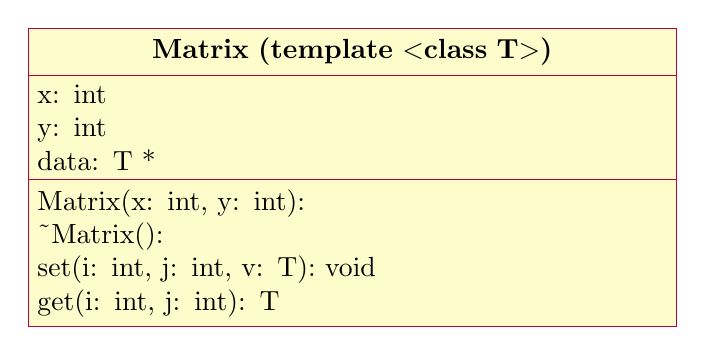
\begin{tikzpicture}
 \begin{class}[text width = 8cm]{Matrix (template $<$class T$>$)}{0,0}
  \attribute{x: int}
	\attribute{y: int}
	\attribute{data: T *}
	
	\operation{Matrix(x: int, y: int):}
	\operation{\~{}Matrix():}
	\operation{set(i: int, j: int, v: T): void}
	\operation{get(i: int, j: int): T}
 \end{class}
\end{tikzpicture}

\paragraph{Point}

The following data structure is a simple point data structure developed for storing the calculated coordinates
for each atom in a Molecule object.\\

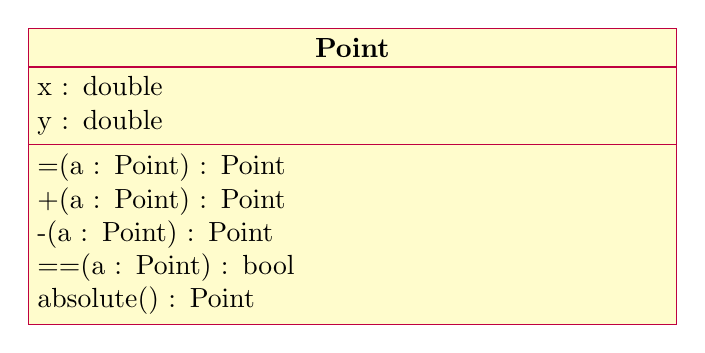
\begin{tikzpicture}
 \begin{class}[text width = 8cm]{Point}{0,0}
  \attribute{x : double}
	\attribute{y : double}
	
	\operation{=(a : Point) : Point}
	\operation{+(a : Point) : Point}
	\operation{-(a : Point) : Point}
	\operation{==(a : Point) : bool}
	\operation{absolute() : Point}
 \end{class}
\end{tikzpicture}

\paragraph{Molecule}

A Molecule class object was implemented for encapsulating all of the data structures necessary for 
defining a molecule with respect to geometry optimisation. a class diagram of the molecule object
is outlined below.\\

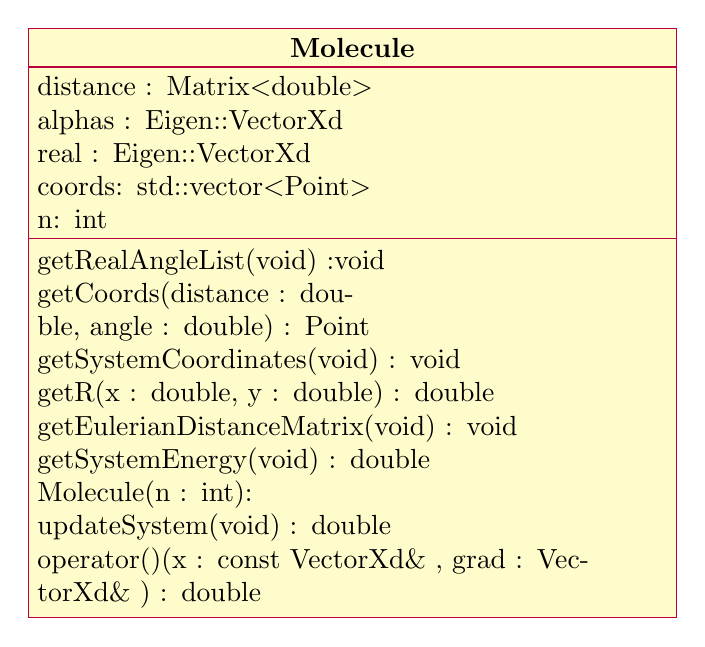
\begin{tikzpicture}
 \begin{class}[text width=8cm]{Molecule}{0,0}
  \attribute{distance : Matrix$<$double$>$}
	\attribute{alphas : Eigen::VectorXd}
	\attribute{real	: Eigen::VectorXd}
	\attribute{coords: std::vector$<$Point$>$}
	\attribute{n: int}
	
	\operation{getRealAngleList(void) :void}
	\operation{getCoords(distance : double, angle : double) : Point}
	\operation{getSystemCoordinates(void) : void}
	\operation{getR(x : double, y : double) : double}
	\operation{getEulerianDistanceMatrix(void) : void}
	\operation{getSystemEnergy(void) : double}
	\operation{Molecule(n : int):}
	\operation{updateSystem(void) : double}
	\operation{operator()(x : const VectorXd\& , grad : VectorXd\& ) : double}
 \end{class}
\end{tikzpicture}

\paragraph{Molecule Function Descriptions}

A number of functions utilised within the Molecule class object are fundamental to the operation of the 
overarching algorithms, and their function will be demonstrated in this section.\\

The following function is used to convert the local alpha variables for each atom
to a global angle, which is required for finding the coordinates of the atom.

\begin{algorithmic}
 \STATE \textit{\textbf{getRealAngleList(void): void}}
 \STATE $real[0] \leftarrow alphas[0]$
 \FOR{$i=1$ to $n$}
  \STATE $real[i] \leftarrow real[i-1] + alphas[i]$
	\IF{$real[i] >= (DEG2RAD * 360)$}
	 \STATE $real[i] -= (DEG2RAD * 360)$
	\ENDIF
 \ENDFOR
\end{algorithmic}

The following function is used to calculate the coordinate values for an atom
given a distance and angle double value.\\

\begin{algorithmic}
 \STATE \textit{\textbf{Molecule::getCoords(dist: double, angle: double): Point}}
 \RETURN $Point(dist*cos(angle),dist*sin(angle))$ 
\end{algorithmic}

The following function is required to calculate the $r(i,j)$ component for
the Lennard-Jones potentials cost function.\\

\begin{algorithmic}
 \STATE \textit{\textbf{Molecule::getR(x: double, y: double): double}}
 \RETURN $sqrt(x*x + y*y)$
\end{algorithmic}

The following function is used to store the atomic distances for each atom
in the lookup table 'distances', to prevent repeat calculations occuring
during the Lennard-Jones potentials calculation and the BFGS derivative
calculation.\\

\begin{algorithmic}
 \STATE \textit{\textbf{Molecule::getEulerianDistanceMatrix(void): void}}
 \FOR{$i=0$ to $n$}
  \FOR{$j=0$ to $n$}
	 \IF{$i==j$}
	  \STATE $distance \leftarrow set(i,j,0.0)$
	 \ELSE
	  \STATE $temp = Point(coords[i] - coords[j])\leftarrow absolute()$
	  \STATE $distance \leftarrow set(i,j,getR(temp.x,temp.y))$
	 \ENDIF
	\ENDFOR
 \ENDFOR
\end{algorithmic}

The following function calculates the Lennard-Jones potentials for each
atom pair, and sums them to form the overall cost of the molecular system.
This function forms the basis of cost for the heuristic search functions.\\\\

\begin{algorithmic}
 \STATE \textit{\textbf{Molecule::getSystemEnergy(void): double}}
 \STATE $V \leftarrow 0.0$
 \FOR{$i=0$ to $n$}
  \FOR{$j=0$ to $j$}
	 \STATE $a \leftarrow (1.0 / pow(distance(i,j),12.0))$
	 \STATE $b \leftarrow (2.0 / pow(distance(i,j),6.0))$
	 \STATE $V \leftarrow V + (a - b)$
	\ENDFOR
 \ENDFOR
 \RETURN $V$
\end{algorithmic}

The following function simply calls all of the update functions
in the correct order of operations, and then returns the current
system energy. This function is called any time the system alphas
are modified, and a new cost evaluation is required.\\

\begin{algorithmic}
 \STATE \textit{\textbf{Molecule::updateSystem(void): double}}
 \STATE $getRealAngleList()$
 \STATE $getSystemCoordinates()$
 \STATE $getEulerianDistanceMatrix()$
 \RETURN $getSystemEnergy()$
\end{algorithmic}

The following is used by the BFGS algorithm to find the derivative of the Lennard-Jones
cost function at a given point during the simulation. Mathematical proof of this algorithm 
and the Lennard-Jones potentials can be found in appendix 1.\\

\begin{algorithmic}
	\STATE \textit{\textbf{Molecule::operator()(x: const VectorXd\&, grad: VectorXd\&): double}}
	\STATE $alphas \leftarrow x$
	\STATE $cost \leftarrow updateSystem()$
	\FOR{$m=0$ to $n$}
	 \STATE $grad[m] = 0.0f$
	 \FOR{$i=0$ to $m-1$}
	  \FOR{$j=m+1$ to $n$}
		 \STATE $a \leftarrow pow(distance(i,j),14.0)$
		 \STATE $b \leftarrow pow(distance(i,j),8.0)$
		 
		 \STATE $c1 \leftarrow (coords[i].x - coords[j].x)$
		 \STATE $c2 \leftarrow (coords[m].y - coords[i].y)$
		 \STATE $d1 \leftarrow (coords[i].y - coords[j].y)$
		 \STATE $d2 \leftarrow (coords[j].x - coords[m].x)$
		 
		 \STATE $c \leftarrow c1 * c2 $
		 \STATE $d \leftarrow d1 * d2 $
		 
		 \STATE $grad[m] \leftarrow grad[m] + (a - b) * (c + d)$
		\ENDFOR
	 \ENDFOR
	 \STATE $grad[m] \leftarrow grad[m] * -12.0$
	\ENDFOR
	\RETURN $cost$
\end{algorithmic}

\subsection{Ordered Single Pass $\alpha$ Optimisation}

\subsubsection{Discussion}

This algorithm follows the application of an extremely strict annealing routine, which randomly
optimises $\alpha_m$ in order $\alpha_0$ ... $\alpha_{n-1}$. This search is performed by iteratively
assigning each $\alpha$ a value in the range of {-180$\degree$...180$\degree$} until a maximum number of
iterations have been performed. Once the maximum is reached the algorithm performs the same steps on the 
next $\alpha$ variable. The pseudocode for this algorithm can be seen below.\\

\subsubsection{Pseudocode}

\begin{algorithmic}
 \STATE \textit{\textbf{BeginOrientatedAnnealing(n: int, iters: int, tempFunc: temp, Molecule mol): double}}
 \FOR{$i=1$ to $n$}
  \STATE $T = temp(n / i)$
	\FOR{$j=0$ to $iters$}
	 \STATE $pE = mol.updateSystem()$
	 \STATE $tv = mol.alphas[i]$
	 \STATE $mol.alphas[i] = random(-180,180)$
	 \STATE $E = mol.updateSystem()$
	 \IF{$E > pE$}
	  \STATE $delta = (E - pE)$
		\IF{$E < 0.0 and (random(0,1) < \exp(-delta/T))$}
		 \STATE // accept new state
		\ELSE
		 \STATE $mol.alphas[i] = tv$
	  \ENDIF
	 \ENDIF
	\ENDFOR
 \ENDFOR
 \RETURN $mol.updateSystem()$
\end{algorithmic}

\subsection{Standard Annealing $\alpha$ Optimisation}

\subsubsection{Discussion}

This is a standard annealing algorithm, following the same strict cooling schedule as the ordered single pass algorithm
for maintaining testing consistency. It is functionally almost identical to the ordered single pass algorithm, however it 
works by altering every $\alpha$ once at each step rather than optimising each $\alpha$ 'iterations' times and moving on to
the next atom permanently.\\ 

\subsubsection{Pseudocode}

\begin{algorithmic}
 \STATE \textit{\textbf{IterativeAnnealing(n: int, iters: int, tempFunc: temp, Molecule mol): double}}
 \FOR{$i=1$ to $iters$}
  \STATE $T = temp(n / i)$
	\FOR{$j=0$ to $n$}
	 \STATE $pE = mol.updateSystem()$
	 \STATE $tv = mol.alphas[j]$
	 \STATE $mol.alphas[j] = random(-180,180)$
	 \STATE $E = mol.updateSystem()$
	 \IF{$E > pE$}
	  \STATE $delta = (E - pE)$
		\IF{$E < 0.0 and (random(0,1) < \exp(-delta/T))$}
		 \STATE // accept new state
		\ELSE
		 \STATE $mol.alphas[j] = tv$
	  \ENDIF
	 \ENDIF
	\ENDFOR
 \ENDFOR
 \RETURN $mol.updateSystem()$
\end{algorithmic}

\subsection{Procedural $\alpha$ Optimisation}

\subsubsection{Discussion}

This algorithm optimises each angle one by one like the first algorithm however instead of searching for the 
correct angle randomly, it checks every angle from {-180$\degree$...180$\degree$} using an angle step size it is given. This 
algorithm is extremely fast, and given a useful iteration size it will always find the global minimum solution
after the use of BFGS when applied to a straight line solution. While this algorithm is very powerful, it does 
not count as a randomised global search algorithm and was developed for benchmarking outside of the known best 
costs and serves to provide an estimate for the level of error present in the other estimations. 

\subsubsection{Pseudocode}

\begin{algorithmic}
 \STATE \textit{\textbf{bruteForceMolecule(n: int, iters: int, Molecule mol): double}}
 \STATE $bestTemp = mol.updateSystem()$
 \FOR{$i=0$ to $n$}
  \STATE $bestAngle = mol.alphas[i]$
	\FOR{$j = -180$ to $180$, $j += 360 / iters$}
	 \STATE $mol.alphas[i] = j$
	 \STATE $curTemp = mol.updateSystem()$
	 \IF{$curTemp < bestTemp$}
	  \STATE $bestAngle = j$
		\STATE $bestTemp = curTemp$
	 \ELSE
	  \STATE $mol.alphas[i] = bestAngle$
	 \ENDIF
	\ENDFOR
 \ENDFOR
 \RETURN $mol.updateSystem()$
\end{algorithmic}

\section{Results}

\subsection{Test Data}

The algorithms were tested on starting solution states in linear, circular and square patterns in order 
to examine how they are able to adjust to different initial solution states. 

For this investigation, tests were performed on all developed algorithms on three different starting
solution states, in order to examine how each algorithm adjusts to different initial solution states. 
Completely random starting states were not fully investigated as finding a reasonable optimum with 
bond crossovers is unreasonably expensive, and it is not economical to randomly generate a solution 
state without crossovers for any solution where $n > 20$. The three initial board states for the $n = 61$ 
case are displayed in figures below.

\subsection{Test Results}

All of the recorded experimental data can be viewed in the appendixes section 3. This section
of the report will discuss these results, and what implications they have about the usefulness
of the algorithms investigated. The main focus of this discussion will be on the $n=61$ case,
however results were computed across the entire range of $2...150$ for each algorithm.\\

The format for this table are as follows:
\begin{enumerate}[noitemsep,topsep=0pt,parsep=0pt,partopsep=0pt]
	\item Atom by Atom Optimisation - Line Start
	\item Atom by Atom Optimisation - Circle Start
	\item Atom by Atom Optimisation - Square Start
	
	\item Iterative Atom Optimisation - Line Start
	\item Iterative Atom Optimisation - Circle Start
	\item Iterative Atom Optimisation - Square Start
	
	\item Brute Force Atom Optimisation - Line Start
	\item Brute Force Atom Optimisation - Circle Start
	\item Brute Force Atom Optimisation - Square Start
	
	\item Atom by Atom Line Start - BFGS
	\item Atom by Atom Circle Start - BFGS
	\item Atom by Atom Square Start - BFGS
	
	\item Iterative Atom Line Start - BFGS
	\item Iterative Atom Circle Start - BFGS
	\item Iterative Atom Square Start - BFGS
	
	\item Brute Force Atom Line Start - BFGS
	\item Brute Force Atom Circle Start - BFGS
	\item Brute Force Atom Square Start - BFGS
\end{enumerate}


\begin{tabular}[t]{c c c c c c}
Atoms & Optimal & Found & Error & Generation & Time(s)\\ 
61 & -171.50 & -155.44 & 9.36 & 50 & 3.72\\
61 & -171.50 & -149.14 & 13.04 & 50 & 3.69\\
61 & -171.50 & -139.09 & 18.90 & 50 & 3.73\\
61 & -171.50 & -106.52 & 37.89 & 50 & 3.73\\
61 & -171.50 & -92.84 & 45.87 & 50 & 3.75\\
61 & -171.50 & -91.94 & 46.39 & 50 & 3.95\\
61 & -171.50 & -169.33 & 1.26 & 50 & 2.02\\
61 & -171.50 & -152.97 & 10.81 & 50 & 2.09\\
61 & -171.50 & -144.09 & 15.98 & 50 & 2.03\\
61 & -171.50 & -164.95 & 3.82 & 50 & 0.97\\
61 & -171.50 & -160.83 & 6.22 & 50 & 1.47\\
61 & -171.50 & -147.83 & 13.80 & 50 & 3.17\\
61 & -171.50 & -117.94 & 31.23 & 50 & 1.41\\
61 & -171.50 & -94.54 & 44.87 & 50 & 6.38\\
61 & -171.50 & -99.28 & 42.11 & 50 & 1.72\\
61 & -171.50 & -171.50 & 0.00 & 50 & 1.01\\
61 & -171.50 & -159.37 & 7.07 & 50 & 1.58\\
61 & -171.50 & -150.51 & 12.24 & 50 & 4.00
\end{tabular}


In this investigation it was observed that for the $n = 61$ straight line solution case, 
before BFGS the atom by atom optimiser had a relative error off the best known solution of 9.36$\%$. This is 
compared to the standard annealing algorithm approach for the same problem, which has a relative error of 
37.89$\%$. After fifty iterations of BFGS are applied, atom by atom optimisation achieves a relative
error of $3.82\%$. For the procedural algorithm with a step size of 50, the initial attempt has a relative error of 
$1.26\%$ and after BFGS is applied it reaches the global minimum and served as the benchmark for the relative error 
for the other test cases.

\section{Performance Analysis}

\section{Bibliography}
\begin{thebibliography}{00}
\bibitem{b1} Dictionary, a. (2018). atom Meaning in the Cambridge English Dictionary. [online] 
Dictionary.cambridge.org.
Available at: https://dictionary.cambridge.org/dictionary/english/atom [Accessed 24 Jul. 2018]
\bibitem{b2} Dictionary, m. (2018). molecule Meaning in the Cambridge English Dictionary. [online] Dictionary.cambridge.org.
Available at: https://dictionary.cambridge.org/dictionary/english/molecule [Accessed 24 Jul. 2018]
\bibitem{b3} shodor.org. (2018). Background Reading for Geometry Optimizations. [online]
Available at: https://www.shodor.org/chemviz/optimization/students/background.html [Accessed 24 Jul. 2018]
\bibitem{b4} Structure.usc.edu. (2018). Minimization and Molecular Dynamics. [online]
Available at: http://structure.usc.edu/mmtk/MMTK 4.html [Accessed 24 Jul. 2018]
\bibitem{b5} Jean, M. (2018). Energy Minimization Methods. [online] About.illinoisstate.edu.
Available at: https://about.illinoisstate.edu/standard/Documents/CHE%20380.37/Handouts/380.37emin.pdf [Accessed
25 Jul. 2018].
\bibitem{b6} Clark, S. (2018). Geometry Optimization. [online] Cmt.dur.ac.uk.
Available at: http://cmt.dur.ac.uk/sjc/thesis dlc/node37.html [Accessed 26 Jul. 2018].
\bibitem{b7} Ul-Haq, Z. (2018). Introduction to Geometry Optimization. [online] Th.fhi-berlin.mpg.de.
Available at: https://th.fhi-berlin.mpg.de/sitesub/meetings/dft-workshop-2016/uploads/Meeting/May 6 Qasmi.pdf
[Accessed 26 Jul. 2018].
\bibitem{b8}Spindynamics.org. (2018). molecular geometry optimization. [online]
Available at: http://spindynamics.org/documents/cqc lecture 6.pdf [Accessed 26 Jul. 2018]
\bibitem{b9}Helgaker, T. (2009). Geometry optimization. [online] Folk.uio.no.
Available at: http://folk.uio.no/helgaker/talks/ESQC09 Optimization.pdf [Accessed 26 Jul. 2018]
\bibitem{b10}Openmopac.net. (2018). The BFGS function optimizer. [online]
Available at: http://openmopac.net/manual/BFGS optimizer.html [Accessed 26 Jul. 2018].
\bibitem{b11}Tcm.phy.cam.ac.uk. (2018). CASTEP Geometry optimization. [online]
Available at: https://tinyurl.com/thcastepgeomopt
[Accessed 26 Jul. 2018].
\bibitem{b12}Cpmd.org. (2018). Geometry Optimization. [online]
Available at: http://www.cpmd.org:81/manual/node80.html [Accessed 26 Jul. 2018].
\bibitem{b13}General methods for geometry and wave function optimization Thomas H. Fischer and Jan Almlof
The Journal of Physical Chemistry 1992 96 (24), 9768-9774 DOI: 10.1021/j100203a036
\bibitem{b14}Tcm.phy.cam.ac.uk. (2018). CASTEP. [online]
Available at: https://preview.tinyurl.com/abtcastep [Accessed 26 Jul. 2018].
\bibitem{b15}Clark, S. J.; Segall, M. D.; Pickard, C. J.; Hasnip, P. J.; Probert, M. J.; Refson, K.; Payne, M. C.
”First principles methods using CASTEP”, Zeitschrift fuer Kristallographie, 220 (5-6), 567-570 (2005
\bibitem{b16}Pullan, WJ 1996, Global optimisation applied to molecular architecture, 
PhD thesis, Central Queensland University, Rockhampton. http://hdl.cqu.edu.au/10018/26734
\end{thebibliography}

\begin{appendix}
\section{Appendix}
\subsection{Proof of Lennard-Jones Potentials First Derivative}

The following proof is provided by the document "Global Optimisation applied to
molecular architecture", by WJ Pullan.[16] \\

The total energy of the system is given by\\

\( V = \sum_{i<j}^{N}(1.0 / r_{ij}^{12} - 2.0/r_{ij}^6)\)\\

Where\\

\( r_{ij} = \sqrt{r_{ij}^2} = \sqrt{x_{ij}^2 + y_{ij}^2} \)\\

Let\\

\(\psi_{k} = \sum_{a=1}^{k} \alpha_{i}\)\\

\(given (x_{0},y_{0}) = (0,0)\) and \( \psi_{0} = 0\) then\\

\(x_{i} = \sum_{k=0}^{i-1}cos(\psi_{k})\)
\(y_{i} = \sum_{k=0}^{i-1}sin(\psi_{k})\)

now\\

\(V_{\alpha_{m}} = -12 \sum_{i<j}(1.0/r_{ij}^{13} - 1.0 / r_{ij}^{7}) r_{ij \alpha_{m}}\)

and\\

\( (r_{ij})_{a_{m}} = ((x_{i}-x_{j})(x_{i}-x_{j})_{a_{m}} + (y_{i} - y_{j})(y_{i}-y_{j})_{a_{m}})/r_{ij}\)\\

Assuming that $j > i$:\\

\( (x_{i} - x_{j})_{a_{m}} = - \sum_{k=i}^{j-1}(cos(\psi_{k}))_{a_{m}} = \sum_{k = max(i,m)}^{j-1} sin(\psi_{k})\)\\

\( (y_{i} - y_{j})_{a_{m}} = - \sum_{k=i}^{j-1}(sin(\psi_{k}))_{a_{m}} = \sum_{k = max(i,m)}^{j-1} cos(\psi_{k})\)\\

Therefore:\\

\( (r_{ij})_{\alpha_{m}} = ((x_{i} - x_{j})(\sum_{k=max(i,m)}^{j-1} sin(\psi_{k}))+(y_{i}-y_{j})(-\sum_{k=max(i,m)}^{j-1}cos(\psi_{k})))/r_{ij}\)\\

Which is zero when $m \leq i$. Assuming $m > i$, we have:\\

\( -\sum_{k=m}^{j-1}cos(\psi_{k} = x_{j} - x_{m}\)\\

\( \sum_{k=m}^{j-1}cos(\psi_{k} = y_{m} - y_{j}\)\\

and\\

\( (r_{ij})_{\alpha_{m}} = ((x_{i}-x_{j})(y_{m}-y_{j}) + (y_{i} - y_{j})(x_{j}-x_{m}))/r_{ij}\)\\

Combining terms we have\\

\( V_{a_{m}} = -12 \sum_{i=0}^{m-1}\sum_{j=m+1}^{n}(1.0/r_{iij}^{14}-1.0/r_{ij}^{8})((x_{i}-x_{j})(y_{m}-y_{j})+(y_{i}-y_{j})(x_{j}-x_{m}))\)\\

\subsection{Utility Programs}

Two utility programs which were used for the testing of this software can be found
in the $/utilities$ directory.

\subsubsection{test.shl}

This script launches the program for the $n = 2$ to $n = 500$ case, and logs all
output to a text file log.txt. It enables the writing of coordinates and alpha
values to the $/coordinates$ and $/alphas$ folder, and saves the best found 
minimum energies to the file 'best.csv'.

\subsubsection{makegraphs.py}

This script takes a file directory as an argument and recursively searches for .csv
files which it can use to graph the coordinates of the containing values on the x,y 
plane. This program is used to generate all of the diagrams used in this report, and
in testing is simply provided the $/coords$ folder. This program has not been written
to handle invalid files or different file formats, and was written specifically for 
the use with this program.

\subsection{Raw Experimental Data For $n = 2$ to $n = 150$ Atom Trials}

This section contains the raw output data of the running program for the 
two to one hundred and fifty atom cases. For each step, at most fifty iterations of 
random alteration were performed and up to fifty iterations of BFGS were applied.
For each 'n' atom case, the tests
were performed in the following order:

\begin{enumerate}[noitemsep,topsep=0pt,parsep=0pt,partopsep=0pt]
	\item Atom by Atom Optimisation - Line Start
	\item Atom by Atom Optimisation - Circle Start
	\item Atom by Atom Optimisation - Square Start
	
	\item Iterative Atom Optimisation - Line Start
	\item Iterative Atom Optimisation - Circle Start
	\item Iterative Atom Optimisation - Square Start
	
	\item Brute Force Atom Optimisation - Line Start
	\item Brute Force Atom Optimisation - Circle Start
	\item Brute Force Atom Optimisation - Square Start
	
	\item Atom by Atom Line Start - BFGS
	\item Atom by Atom Circle Start - BFGS
	\item Atom by Atom Square Start - BFGS
	
	\item Iterative Atom Line Start - BFGS
	\item Iterative Atom Circle Start - BFGS
	\item Iterative Atom Square Start - BFGS
	
	\item Brute Force Atom Line Start - BFGS
	\item Brute Force Atom Circle Start - BFGS
	\item Brute Force Atom Square Start - BFGS
\end{enumerate}

\begin{longtable}{llllll}
Atoms & Optimal & Found & Error & Gen & Time \\
\endfirsthead
%
\endhead
%
2 & -1.00 & -1.00 & -0.00 & 50 & 0.00 \\
2 & -1.00 & -1.00 & -0.00 & 50 & 0.00 \\
2 & -1.00 & -1.00 & -0.00 & 50 & 0.00 \\
2 & -1.00 & -1.00 & -0.00 & 50 & 0.00 \\
2 & -1.00 & -1.00 & -0.00 & 50 & 0.00 \\
2 & -1.00 & -1.00 & -0.00 & 50 & 0.00 \\
2 & -1.00 & -1.00 & -0.00 & 50 & 0.00 \\
2 & -1.00 & -1.00 & -0.00 & 50 & 0.00 \\
2 & -1.00 & -1.00 & -0.00 & 50 & 0.00 \\
2 & -1.00 & -1.00 & -0.00 & 50 & 0.00 \\
2 & -1.00 & -1.00 & -0.00 & 50 & 0.00 \\
2 & -1.00 & -1.00 & -0.00 & 50 & 0.00 \\
2 & -1.00 & -1.00 & -0.00 & 50 & 0.00 \\
2 & -1.00 & -1.00 & -0.00 & 50 & 0.00 \\
2 & -1.00 & -1.00 & -0.00 & 50 & 0.00 \\
2 & -1.00 & -1.00 & -0.00 & 50 & 0.00 \\
2 & -1.00 & -1.00 & -0.00 & 50 & 0.00 \\
2 & -1.00 & -1.00 & -0.00 & 50 & 0.00 \\
Atoms & Optimal & Found & Error & Gen & Time \\
3 & -3.00 & -2.88 & 4.10 & 50 & 0.00 \\
3 & -3.00 & -3.00 & -0.00 & 50 & 0.00 \\
3 & -3.00 & -2.90 & 3.50 & 50 & 0.00 \\
3 & -3.00 & -2.99 & 0.25 & 50 & 0.00 \\
3 & -3.00 & -3.00 & -0.00 & 50 & 0.00 \\
3 & -3.00 & -3.00 & -0.00 & 50 & 0.00 \\
3 & -3.00 & -2.99 & 0.44 & 50 & 0.01 \\
3 & -3.00 & -3.00 & -0.00 & 50 & 0.00 \\
3 & -3.00 & -2.99 & 0.43 & 50 & 0.00 \\
3 & -3.00 & -2.88 & 4.10 & 50 & 0.00 \\
3 & -3.00 & -3.00 & -0.00 & 50 & 0.00 \\
3 & -3.00 & -2.90 & 3.50 & 50 & 0.00 \\
3 & -3.00 & -2.99 & 0.25 & 50 & 0.00 \\
3 & -3.00 & -3.00 & -0.00 & 50 & 0.00 \\
3 & -3.00 & -3.00 & -0.00 & 50 & 0.00 \\
3 & -3.00 & -2.99 & 0.44 & 50 & 0.00 \\
3 & -3.00 & -3.00 & -0.00 & 50 & 0.00 \\
3 & -3.00 & -2.99 & 0.43 & 50 & 0.00 \\
Atoms & Optimal & Found & Error & Gen & Time \\
4 & -5.06 & -4.86 & 3.93 & 50 & 0.00 \\
4 & -5.06 & -4.47 & 11.65 & 50 & 0.00 \\
4 & -5.06 & -4.47 & 11.63 & 50 & 0.00 \\
4 & -5.06 & -5.03 & 0.62 & 50 & 0.00 \\
4 & -5.06 & -4.82 & 4.69 & 50 & 0.00 \\
4 & -5.06 & -4.47 & 11.63 & 50 & 0.00 \\
4 & -5.06 & -5.06 & 0.02 & 50 & 0.00 \\
4 & -5.06 & -4.47 & 11.65 & 50 & 0.00 \\
4 & -5.06 & -4.47 & 11.63 & 50 & 0.00 \\
4 & -5.06 & -4.96 & 1.88 & 50 & 0.00 \\
4 & -5.06 & -4.47 & 11.59 & 50 & 0.00 \\
4 & -5.06 & -4.47 & 11.63 & 50 & 0.00 \\
4 & -5.06 & -5.03 & 0.62 & 50 & 0.00 \\
4 & -5.06 & -4.82 & 4.69 & 50 & 0.00 \\
4 & -5.06 & -4.47 & 11.63 & 50 & 0.00 \\
4 & -5.06 & -5.06 & -0.00 & 50 & 0.01 \\
4 & -5.06 & -4.47 & 11.59 & 50 & 0.00 \\
4 & -5.06 & -4.47 & 11.63 & 50 & 0.00 \\
Atoms & Optimal & Found & Error & Gen & Time \\
5 & -7.16 & -7.01 & 2.16 & 50 & 0.00 \\
5 & -7.16 & -4.85 & 32.27 & 50 & 0.00 \\
5 & -7.16 & -6.53 & 8.89 & 50 & 0.00 \\
5 & -7.16 & -6.54 & 8.70 & 50 & 0.00 \\
5 & -7.16 & -5.55 & 22.57 & 50 & 0.00 \\
5 & -7.16 & -6.52 & 9.04 & 50 & 0.00 \\
5 & -7.16 & -7.15 & 0.15 & 50 & 0.00 \\
5 & -7.16 & -5.54 & 22.65 & 50 & 0.00 \\
5 & -7.16 & -6.54 & 8.68 & 50 & 0.00 \\
5 & -7.16 & -7.14 & 0.39 & 50 & 0.00 \\
5 & -7.16 & -4.85 & 32.27 & 50 & 0.01 \\
5 & -7.16 & -6.55 & 8.53 & 50 & 0.00 \\
5 & -7.16 & -6.55 & 8.51 & 50 & 0.00 \\
5 & -7.16 & -5.87 & 18.09 & 50 & 0.00 \\
5 & -7.16 & -6.52 & 8.97 & 50 & 0.02 \\
5 & -7.16 & -7.16 & -0.00 & 50 & 0.00 \\
5 & -7.16 & -5.91 & 17.56 & 50 & 0.00 \\
5 & -7.16 & -6.55 & 8.62 & 50 & 0.00 \\
Atoms & Optimal & Found & Error & Gen & Time \\
6 & -9.35 & -9.20 & 1.70 & 50 & 0.00 \\
6 & -9.35 & -9.15 & 2.23 & 50 & 0.00 \\
6 & -9.35 & -7.17 & 23.36 & 50 & 0.00 \\
6 & -9.35 & -7.93 & 15.22 & 50 & 0.00 \\
6 & -9.35 & -9.35 & 0.02 & 50 & 0.02 \\
6 & -9.35 & -8.03 & 14.14 & 50 & 0.00 \\
6 & -9.35 & -9.34 & 0.20 & 50 & 0.00 \\
6 & -9.35 & -9.35 & 0.02 & 50 & 0.00 \\
6 & -9.35 & -7.99 & 14.64 & 50 & 0.00 \\
6 & -9.35 & -9.32 & 0.36 & 50 & 0.00 \\
6 & -9.35 & -9.35 & -0.00 & 50 & 0.01 \\
6 & -9.35 & -8.67 & 7.33 & 50 & 0.00 \\
6 & -9.35 & -8.23 & 11.97 & 50 & 0.02 \\
6 & -9.35 & -9.35 & 0.00 & 50 & 0.00 \\
6 & -9.35 & -8.67 & 7.37 & 50 & 0.00 \\
6 & -9.35 & -9.35 & 0.10 & 50 & 0.02 \\
6 & -9.35 & -9.35 & 0.00 & 50 & 0.00 \\
6 & -9.35 & -8.66 & 7.40 & 50 & 0.01 \\
Atoms & Optimal & Found & Error & Gen & Time \\
7 & -12.52 & -12.10 & 3.33 & 50 & 0.00 \\
7 & -12.52 & -12.24 & 2.22 & 50 & 0.00 \\
7 & -12.52 & -10.15 & 18.95 & 50 & 0.00 \\
7 & -12.52 & -10.81 & 13.62 & 50 & 0.00 \\
7 & -12.52 & -12.26 & 2.04 & 50 & 0.01 \\
7 & -12.52 & -10.11 & 19.21 & 50 & 0.00 \\
7 & -12.52 & -12.48 & 0.33 & 50 & 0.00 \\
7 & -12.52 & -11.56 & 7.66 & 50 & 0.00 \\
7 & -12.52 & -10.17 & 18.76 & 50 & 0.02 \\
7 & -12.52 & -12.48 & 0.32 & 50 & 0.00 \\
7 & -12.52 & -12.37 & 1.20 & 50 & 0.01 \\
7 & -12.52 & -11.03 & 11.93 & 50 & 0.00 \\
7 & -12.52 & -12.40 & 0.94 & 50 & 0.02 \\
7 & -12.52 & -12.52 & -0.00 & 50 & 0.00 \\
7 & -12.52 & -10.21 & 18.46 & 50 & 0.02 \\
7 & -12.52 & -12.52 & 0.02 & 50 & 0.01 \\
7 & -12.52 & -12.50 & 0.17 & 50 & 0.00 \\
7 & -12.52 & -11.09 & 11.39 & 50 & 0.02 \\
Atoms & Optimal & Found & Error & Gen & Time \\
8 & -14.68 & -14.20 & 3.25 & 50 & 0.00 \\
8 & -14.68 & -12.81 & 12.71 & 50 & 0.01 \\
8 & -14.68 & -11.72 & 20.11 & 50 & 0.00 \\
8 & -14.68 & -11.62 & 20.82 & 50 & 0.00 \\
8 & -14.68 & -12.75 & 13.10 & 50 & 0.02 \\
8 & -14.68 & -13.04 & 11.16 & 50 & 0.00 \\
8 & -14.68 & -14.61 & 0.45 & 50 & 0.01 \\
8 & -14.68 & -12.39 & 15.60 & 50 & 0.00 \\
8 & -14.68 & -11.92 & 18.80 & 50 & 0.00 \\
8 & -14.68 & -14.63 & 0.34 & 50 & 0.02 \\
8 & -14.68 & -14.68 & -0.00 & 50 & 0.00 \\
8 & -14.68 & -13.22 & 9.91 & 50 & 0.02 \\
8 & -14.68 & -11.64 & 20.71 & 50 & 0.03 \\
8 & -14.68 & -12.77 & 13.01 & 50 & 0.02 \\
8 & -14.68 & -13.09 & 10.80 & 50 & 0.01 \\
8 & -14.68 & -14.66 & 0.11 & 50 & 0.02 \\
8 & -14.68 & -14.66 & 0.14 & 50 & 0.00 \\
8 & -14.68 & -12.22 & 16.71 & 50 & 0.01 \\
Atoms & Optimal & Found & Error & Gen & Time \\
9 & -16.85 & -16.31 & 3.26 & 50 & 0.01 \\
9 & -16.85 & -14.89 & 11.68 & 50 & 0.00 \\
9 & -16.85 & -14.00 & 16.94 & 50 & 0.02 \\
9 & -16.85 & -13.28 & 21.19 & 50 & 0.01 \\
9 & -16.85 & -12.96 & 23.13 & 50 & 0.00 \\
9 & -16.85 & -13.31 & 21.03 & 50 & 0.02 \\
9 & -16.85 & -16.81 & 0.29 & 50 & 0.00 \\
9 & -16.85 & -13.89 & 17.60 & 50 & 0.00 \\
9 & -16.85 & -13.93 & 17.37 & 50 & 0.02 \\
9 & -16.85 & -16.82 & 0.21 & 50 & 0.00 \\
9 & -16.85 & -16.81 & 0.25 & 50 & 0.01 \\
9 & -16.85 & -15.32 & 9.10 & 50 & 0.02 \\
9 & -16.85 & -11.64 & 30.96 & 50 & 0.03 \\
9 & -16.85 & -16.04 & 4.84 & 50 & 0.00 \\
9 & -16.85 & -15.07 & 10.61 & 50 & 0.03 \\
9 & -16.85 & -16.85 & -0.00 & 50 & 0.02 \\
9 & -16.85 & -13.85 & 17.82 & 50 & 0.03 \\
9 & -16.85 & -15.43 & 8.47 & 50 & 0.02 \\
Atoms & Optimal & Found & Error & Gen & Time \\
10 & -20.08 & -19.23 & 4.21 & 50 & 0.01 \\
10 & -20.08 & -17.68 & 11.95 & 50 & 0.02 \\
10 & -20.08 & -15.86 & 20.97 & 50 & 0.01 \\
10 & -20.08 & -14.78 & 26.39 & 50 & 0.00 \\
10 & -20.08 & -16.13 & 19.66 & 50 & 0.02 \\
10 & -20.08 & -15.18 & 24.38 & 50 & 0.02 \\
10 & -20.08 & -20.02 & 0.26 & 50 & 0.01 \\
10 & -20.08 & -18.42 & 8.23 & 50 & 0.00 \\
10 & -20.08 & -16.06 & 19.99 & 50 & 0.02 \\
10 & -20.08 & -20.07 & 0.05 & 50 & 0.02 \\
10 & -20.08 & -20.07 & 0.03 & 50 & 0.00 \\
10 & -20.08 & -16.36 & 18.52 & 50 & 0.03 \\
10 & -20.08 & -12.62 & 37.12 & 50 & 0.03 \\
10 & -20.08 & -16.57 & 17.46 & 50 & 0.03 \\
10 & -20.08 & -17.11 & 14.77 & 50 & 0.03 \\
10 & -20.08 & -20.08 & -0.00 & 50 & 0.03 \\
10 & -20.08 & -18.75 & 6.60 & 50 & 0.03 \\
10 & -20.08 & -17.58 & 12.41 & 50 & 0.02 \\
Atoms & Optimal & Found & Error & Gen & Time \\
11 & -22.31 & -21.46 & 3.81 & 50 & 0.01 \\
11 & -22.31 & -19.27 & 13.64 & 50 & 0.02 \\
11 & -22.31 & -16.95 & 24.04 & 50 & 0.01 \\
11 & -22.31 & -17.40 & 21.99 & 50 & 0.02 \\
11 & -22.31 & -18.39 & 17.57 & 50 & 0.03 \\
11 & -22.31 & -17.02 & 23.70 & 50 & 0.02 \\
11 & -22.31 & -22.26 & 0.25 & 50 & 0.00 \\
11 & -22.31 & -19.70 & 11.72 & 50 & 0.02 \\
11 & -22.31 & -17.68 & 20.75 & 50 & 0.01 \\
11 & -22.31 & -22.28 & 0.15 & 50 & 0.00 \\
11 & -22.31 & -20.15 & 9.70 & 50 & 0.05 \\
11 & -22.31 & -20.15 & 9.70 & 50 & 0.02 \\
11 & -22.31 & -17.75 & 20.43 & 50 & 0.05 \\
11 & -22.31 & -18.37 & 17.65 & 50 & 0.06 \\
11 & -22.31 & -20.37 & 8.70 & 50 & 0.03 \\
11 & -22.31 & -22.31 & -0.00 & 50 & 0.05 \\
11 & -22.31 & -20.25 & 9.22 & 50 & 0.02 \\
11 & -22.31 & -18.19 & 18.49 & 50 & 0.05 \\
Atoms & Optimal & Found & Error & Gen & Time \\
12 & -25.53 & -25.11 & 1.65 & 50 & 0.01 \\
12 & -25.53 & -22.47 & 11.98 & 50 & 0.02 \\
12 & -25.53 & -22.01 & 13.78 & 50 & 0.03 \\
12 & -25.53 & -19.64 & 23.05 & 50 & 0.02 \\
12 & -25.53 & -19.29 & 24.45 & 50 & 0.03 \\
12 & -25.53 & -19.35 & 24.19 & 50 & 0.03 \\
12 & -25.53 & -25.44 & 0.35 & 50 & 0.02 \\
12 & -25.53 & -22.71 & 11.03 & 50 & 0.00 \\
12 & -25.53 & -21.57 & 15.49 & 50 & 0.01 \\
12 & -25.53 & -25.52 & 0.01 & 50 & 0.05 \\
12 & -25.53 & -23.00 & 9.91 & 50 & 0.06 \\
12 & -25.53 & -22.60 & 11.47 & 50 & 0.01 \\
12 & -25.53 & -19.71 & 22.79 & 50 & 0.06 \\
12 & -25.53 & -22.96 & 10.05 & 50 & 0.03 \\
12 & -25.53 & -20.25 & 20.68 & 50 & 0.06 \\
12 & -25.53 & -25.53 & -0.00 & 50 & 0.06 \\
12 & -25.53 & -23.23 & 8.99 & 50 & 0.05 \\
12 & -25.53 & -22.15 & 13.23 & 50 & 0.05 \\
Atoms & Optimal & Found & Error & Gen & Time \\
13 & -27.75 & -26.73 & 3.69 & 50 & 0.03 \\
13 & -27.75 & -24.46 & 11.88 & 50 & 0.03 \\
13 & -27.75 & -24.33 & 12.33 & 50 & 0.03 \\
13 & -27.75 & -21.03 & 24.24 & 50 & 0.03 \\
13 & -27.75 & -21.24 & 23.45 & 50 & 0.03 \\
13 & -27.75 & -20.47 & 26.23 & 50 & 0.03 \\
13 & -27.75 & -27.66 & 0.32 & 50 & 0.02 \\
13 & -27.75 & -24.46 & 11.87 & 50 & 0.01 \\
13 & -27.75 & -24.25 & 12.62 & 50 & 0.02 \\
13 & -27.75 & -27.38 & 1.34 & 50 & 0.03 \\
13 & -27.75 & -25.12 & 9.48 & 50 & 0.06 \\
13 & -27.75 & -24.91 & 10.24 & 50 & 0.06 \\
13 & -27.75 & -21.49 & 22.59 & 50 & 0.06 \\
13 & -27.75 & -21.93 & 20.99 & 50 & 0.06 \\
13 & -27.75 & -21.15 & 23.80 & 50 & 0.08 \\
13 & -27.75 & -27.75 & -0.00 & 50 & 0.08 \\
13 & -27.75 & -25.69 & 7.44 & 50 & 0.09 \\
13 & -27.75 & -24.57 & 11.46 & 50 & 0.08 \\
Atoms & Optimal & Found & Error & Gen & Time \\
14 & -30.98 & -29.90 & 3.51 & 50 & 0.03 \\
14 & -30.98 & -26.15 & 15.61 & 50 & 0.03 \\
14 & -30.98 & -25.44 & 17.89 & 50 & 0.05 \\
14 & -30.98 & -23.76 & 23.30 & 50 & 0.03 \\
14 & -30.98 & -21.25 & 31.43 & 50 & 0.05 \\
14 & -30.98 & -23.08 & 25.51 & 50 & 0.05 \\
14 & -30.98 & -30.89 & 0.31 & 50 & 0.02 \\
14 & -30.98 & -27.20 & 12.21 & 50 & 0.01 \\
14 & -30.98 & -24.63 & 20.50 & 50 & 0.03 \\
14 & -30.98 & -30.62 & 1.17 & 50 & 0.09 \\
14 & -30.98 & -27.35 & 11.72 & 50 & 0.06 \\
14 & -30.98 & -26.95 & 13.03 & 50 & 0.03 \\
14 & -30.98 & -23.98 & 22.60 & 50 & 0.09 \\
14 & -30.98 & -21.56 & 30.42 & 50 & 0.09 \\
14 & -30.98 & -27.16 & 12.33 & 50 & 0.06 \\
14 & -30.98 & -30.98 & -0.00 & 50 & 0.09 \\
14 & -30.98 & -28.42 & 8.27 & 50 & 0.03 \\
14 & -30.98 & -25.66 & 17.19 & 50 & 0.09 \\
Atoms & Optimal & Found & Error & Gen & Time \\
15 & -33.23 & -33.09 & 0.44 & 50 & 0.05 \\
15 & -33.23 & -28.85 & 13.19 & 50 & 0.05 \\
15 & -33.23 & -28.64 & 13.81 & 50 & 0.05 \\
15 & -33.23 & -24.03 & 27.68 & 50 & 0.05 \\
15 & -33.23 & -20.51 & 38.29 & 50 & 0.05 \\
15 & -33.23 & -21.48 & 35.37 & 50 & 0.05 \\
15 & -33.23 & -33.12 & 0.33 & 50 & 0.03 \\
15 & -33.23 & -28.75 & 13.50 & 50 & 0.03 \\
15 & -33.23 & -29.84 & 10.22 & 50 & 0.03 \\
15 & -33.23 & -33.23 & -0.00 & 50 & 0.06 \\
15 & -33.23 & -30.57 & 8.00 & 50 & 0.05 \\
15 & -33.23 & -29.50 & 11.22 & 50 & 0.06 \\
15 & -33.23 & -25.59 & 22.99 & 50 & 0.11 \\
15 & -33.23 & -23.03 & 30.71 & 50 & 0.09 \\
15 & -33.23 & -21.69 & 34.73 & 50 & 0.12 \\
15 & -33.23 & -33.22 & 0.05 & 50 & 0.09 \\
15 & -33.23 & -29.58 & 11.00 & 50 & 0.11 \\
15 & -33.23 & -30.29 & 8.87 & 50 & 0.14 \\
Atoms & Optimal & Found & Error & Gen & Time \\
16 & -36.45 & -33.59 & 7.85 & 50 & 0.05 \\
16 & -36.45 & -32.87 & 9.82 & 50 & 0.06 \\
16 & -36.45 & -29.35 & 19.47 & 50 & 0.06 \\
16 & -36.45 & -22.54 & 38.16 & 50 & 0.06 \\
16 & -36.45 & -26.96 & 26.04 & 50 & 0.06 \\
16 & -36.45 & -27.79 & 23.78 & 50 & 0.06 \\
16 & -36.45 & -36.30 & 0.41 & 50 & 0.03 \\
16 & -36.45 & -31.46 & 13.69 & 50 & 0.03 \\
16 & -36.45 & -31.86 & 12.61 & 50 & 0.03 \\
16 & -36.45 & -34.02 & 6.68 & 50 & 0.14 \\
16 & -36.45 & -33.13 & 9.12 & 50 & 0.16 \\
16 & -36.45 & -31.17 & 14.50 & 50 & 0.12 \\
16 & -36.45 & -23.07 & 36.70 & 50 & 0.12 \\
16 & -36.45 & -29.42 & 19.29 & 50 & 0.11 \\
16 & -36.45 & -29.38 & 19.39 & 50 & 0.05 \\
16 & -36.45 & -36.45 & -0.00 & 50 & 0.14 \\
16 & -36.45 & -32.54 & 10.74 & 50 & 0.12 \\
16 & -36.45 & -32.20 & 11.68 & 50 & 0.17 \\
Atoms & Optimal & Found & Error & Gen & Time \\
17 & -38.69 & -36.12 & 6.65 & 50 & 0.08 \\
17 & -38.69 & -34.36 & 11.19 & 50 & 0.06 \\
17 & -38.69 & -31.68 & 18.13 & 50 & 0.08 \\
17 & -38.69 & -28.78 & 25.63 & 50 & 0.08 \\
17 & -38.69 & -23.37 & 39.60 & 50 & 0.08 \\
17 & -38.69 & -27.56 & 28.78 & 50 & 0.06 \\
17 & -38.69 & -38.55 & 0.38 & 50 & 0.05 \\
17 & -38.69 & -32.65 & 15.61 & 50 & 0.03 \\
17 & -38.69 & -33.55 & 13.30 & 50 & 0.05 \\
17 & -38.69 & -38.29 & 1.04 & 50 & 0.11 \\
17 & -38.69 & -34.46 & 10.95 & 50 & 0.16 \\
17 & -38.69 & -32.93 & 14.91 & 50 & 0.12 \\
17 & -38.69 & -31.72 & 18.02 & 50 & 0.11 \\
17 & -38.69 & -26.30 & 32.02 & 50 & 0.03 \\
17 & -38.69 & -27.96 & 27.73 & 50 & 0.12 \\
17 & -38.69 & -38.69 & -0.00 & 50 & 0.17 \\
17 & -38.69 & -33.80 & 12.66 & 50 & 0.19 \\
17 & -38.69 & -34.09 & 11.89 & 50 & 0.19 \\
Atoms & Optimal & Found & Error & Gen & Time \\
18 & -42.01 & -37.92 & 9.74 & 50 & 0.09 \\
18 & -42.01 & -34.40 & 18.10 & 50 & 0.08 \\
18 & -42.01 & -35.24 & 16.11 & 50 & 0.09 \\
18 & -42.01 & -24.15 & 42.50 & 50 & 0.08 \\
18 & -42.01 & -31.29 & 25.51 & 50 & 0.09 \\
18 & -42.01 & -28.27 & 32.71 & 50 & 0.08 \\
18 & -42.01 & -41.80 & 0.49 & 50 & 0.05 \\
18 & -42.01 & -36.77 & 12.48 & 50 & 0.06 \\
18 & -42.01 & -34.10 & 18.83 & 50 & 0.05 \\
18 & -42.01 & -38.11 & 9.28 & 50 & 0.23 \\
18 & -42.01 & -37.61 & 10.46 & 50 & 0.06 \\
18 & -42.01 & -36.11 & 14.03 & 50 & 0.17 \\
18 & -42.01 & -29.38 & 30.07 & 50 & 0.09 \\
18 & -42.01 & -33.65 & 19.90 & 50 & 0.12 \\
18 & -42.01 & -29.37 & 30.08 & 50 & 0.20 \\
18 & -42.01 & -42.01 & -0.00 & 50 & 0.14 \\
18 & -42.01 & -37.24 & 11.35 & 50 & 0.17 \\
18 & -42.01 & -34.72 & 17.36 & 50 & 0.20 \\
Atoms & Optimal & Found & Error & Gen & Time \\
19 & -45.26 & -43.21 & 4.53 & 50 & 0.11 \\
19 & -45.26 & -41.23 & 8.90 & 50 & 0.09 \\
19 & -45.26 & -35.41 & 21.76 & 50 & 0.11 \\
19 & -45.26 & -30.24 & 33.18 & 50 & 0.09 \\
19 & -45.26 & -32.91 & 27.29 & 50 & 0.11 \\
19 & -45.26 & -28.63 & 36.75 & 50 & 0.11 \\
19 & -45.26 & -44.99 & 0.59 & 50 & 0.06 \\
19 & -45.26 & -37.99 & 16.06 & 50 & 0.05 \\
19 & -45.26 & -36.40 & 19.57 & 50 & 0.06 \\
19 & -45.26 & -43.57 & 3.74 & 50 & 0.23 \\
19 & -45.26 & -41.82 & 7.59 & 50 & 0.17 \\
19 & -45.26 & -37.25 & 17.70 & 50 & 0.25 \\
19 & -45.26 & -31.49 & 30.43 & 50 & 0.23 \\
19 & -45.26 & -33.55 & 25.88 & 50 & 0.27 \\
19 & -45.26 & -28.82 & 36.32 & 50 & 0.28 \\
19 & -45.26 & -45.26 & -0.00 & 50 & 0.19 \\
19 & -45.26 & -38.30 & 15.38 & 50 & 0.22 \\
19 & -45.26 & -37.04 & 18.16 & 50 & 0.23 \\
Atoms & Optimal & Found & Error & Gen & Time \\
20 & -47.49 & -47.28 & 0.43 & 50 & 0.12 \\
20 & -47.49 & -41.67 & 12.26 & 50 & 0.11 \\
20 & -47.49 & -36.91 & 22.27 & 50 & 0.12 \\
20 & -47.49 & -36.47 & 23.20 & 50 & 0.12 \\
20 & -47.49 & 308.72 & 750.08 & 50 & 0.12 \\
20 & -47.49 & -33.23 & 30.03 & 50 & 0.11 \\
20 & -47.49 & -47.21 & 0.59 & 50 & 0.08 \\
20 & -47.49 & -41.00 & 13.67 & 50 & 0.06 \\
20 & -47.49 & -38.14 & 19.69 & 50 & 0.06 \\
20 & -47.49 & -47.44 & 0.10 & 50 & 0.25 \\
20 & -47.49 & -42.78 & 9.92 & 50 & 0.20 \\
20 & -47.49 & -37.62 & 20.78 & 50 & 0.31 \\
20 & -47.49 & -37.67 & 20.67 & 50 & 0.28 \\
20 & -47.49 & 161.76 & 440.62 & 50 & 0.23 \\
20 & -47.49 & -33.64 & 29.17 & 50 & 0.33 \\
20 & -47.49 & -47.49 & -0.00 & 50 & 0.23 \\
20 & -47.49 & -41.89 & 11.80 & 50 & 0.20 \\
20 & -47.49 & -39.74 & 16.33 & 50 & 0.28 \\
Atoms & Optimal & Found & Error & Gen & Time \\
21 & -50.73 & -48.46 & 4.46 & 50 & 0.14 \\
21 & -50.73 & -43.04 & 15.14 & 50 & 0.14 \\
21 & -50.73 & -43.05 & 15.14 & 50 & 0.14 \\
21 & -50.73 & -29.07 & 42.69 & 50 & 0.14 \\
21 & -50.73 & -26.31 & 48.14 & 50 & 0.14 \\
21 & -50.73 & -36.16 & 28.71 & 50 & 0.14 \\
21 & -50.73 & -50.43 & 0.58 & 50 & 0.08 \\
21 & -50.73 & -45.45 & 10.40 & 50 & 0.06 \\
21 & -50.73 & -42.72 & 15.78 & 50 & 0.08 \\
21 & -50.73 & -50.25 & 0.93 & 50 & 0.20 \\
21 & -50.73 & -44.21 & 12.85 & 50 & 0.33 \\
21 & -50.73 & -43.87 & 13.52 & 50 & 0.20 \\
21 & -50.73 & -30.22 & 40.42 & 50 & 0.19 \\
21 & -50.73 & -26.50 & 47.75 & 50 & 0.12 \\
21 & -50.73 & -36.29 & 28.46 & 50 & 0.38 \\
21 & -50.73 & -50.73 & -0.00 & 50 & 0.27 \\
21 & -50.73 & -45.83 & 9.65 & 50 & 0.34 \\
21 & -50.73 & -43.33 & 14.59 & 50 & 0.30 \\
Atoms & Optimal & Found & Error & Gen & Time \\
22 & -52.97 & -50.31 & 5.02 & 50 & 0.16 \\
22 & -52.97 & -47.69 & 9.97 & 50 & 0.16 \\
22 & -52.97 & -43.93 & 17.07 & 50 & 0.16 \\
22 & -52.97 & -37.72 & 28.78 & 50 & 0.17 \\
22 & -52.97 & -39.42 & 25.58 & 50 & 0.16 \\
22 & -52.97 & -28.68 & 45.86 & 50 & 0.16 \\
22 & -52.97 & -52.68 & 0.56 & 50 & 0.09 \\
22 & -52.97 & -47.91 & 9.55 & 50 & 0.08 \\
22 & -52.97 & -45.77 & 13.59 & 50 & 0.09 \\
22 & -52.97 & -51.60 & 2.58 & 50 & 0.41 \\
22 & -52.97 & -48.32 & 8.78 & 50 & 0.30 \\
22 & -52.97 & -45.33 & 14.43 & 50 & 0.31 \\
22 & -52.97 & -39.44 & 25.55 & 50 & 0.27 \\
22 & -52.97 & -39.92 & 24.63 & 50 & 0.44 \\
22 & -52.97 & -30.18 & 43.03 & 50 & 0.25 \\
22 & -52.97 & -52.97 & -0.00 & 50 & 0.31 \\
22 & -52.97 & -50.31 & 5.03 & 50 & 0.14 \\
22 & -52.97 & -47.76 & 9.84 & 50 & 0.20 \\
Atoms & Optimal & Found & Error & Gen & Time \\
23 & -56.29 & -50.11 & 10.98 & 50 & 0.19 \\
23 & -56.29 & -50.44 & 10.40 & 50 & 0.19 \\
23 & -56.29 & -43.04 & 23.54 & 50 & 0.19 \\
23 & -56.29 & -38.88 & 30.94 & 50 & 0.19 \\
23 & -56.29 & -40.55 & 27.96 & 50 & 0.19 \\
23 & -56.29 & -36.70 & 34.80 & 50 & 0.20 \\
23 & -56.29 & -55.98 & 0.55 & 50 & 0.09 \\
23 & -56.29 & -49.98 & 11.20 & 50 & 0.09 \\
23 & -56.29 & -46.56 & 17.28 & 50 & 0.11 \\
23 & -56.29 & -53.43 & 5.09 & 50 & 0.38 \\
23 & -56.29 & -52.42 & 6.88 & 50 & 0.14 \\
23 & -56.29 & -43.69 & 22.39 & 50 & 0.47 \\
23 & -56.29 & -40.97 & 27.22 & 50 & 0.36 \\
23 & -56.29 & -43.08 & 23.47 & 50 & 0.14 \\
23 & -56.29 & -36.87 & 34.50 & 50 & 0.48 \\
23 & -56.29 & -56.29 & -0.00 & 50 & 0.23 \\
23 & -56.29 & -51.39 & 8.71 & 50 & 0.31 \\
23 & -56.29 & -47.29 & 15.99 & 50 & 0.42 \\
Atoms & Optimal & Found & Error & Gen & Time \\
24 & -59.56 & -57.11 & 4.12 & 50 & 0.20 \\
24 & -59.56 & -53.49 & 10.20 & 50 & 0.22 \\
24 & -59.56 & -48.19 & 19.09 & 50 & 0.20 \\
24 & -59.56 & -42.30 & 28.98 & 50 & 0.22 \\
24 & -59.56 & -31.30 & 47.44 & 50 & 0.22 \\
24 & -59.56 & -35.78 & 39.92 & 50 & 0.22 \\
24 & -59.56 & -59.24 & 0.54 & 50 & 0.12 \\
24 & -59.56 & -52.46 & 11.93 & 50 & 0.11 \\
24 & -59.56 & -49.84 & 16.32 & 50 & 0.11 \\
24 & -59.56 & -58.88 & 1.16 & 50 & 0.33 \\
24 & -59.56 & -54.40 & 8.67 & 50 & 0.53 \\
24 & -59.56 & -49.40 & 17.06 & 50 & 0.45 \\
24 & -59.56 & -48.08 & 19.27 & 50 & 0.30 \\
24 & -59.56 & -31.50 & 47.11 & 50 & 0.52 \\
24 & -59.56 & -36.57 & 38.60 & 50 & 0.42 \\
24 & -59.56 & -59.56 & -0.00 & 50 & 0.33 \\
24 & -59.56 & -53.51 & 10.17 & 50 & 0.52 \\
24 & -59.56 & -50.79 & 14.73 & 50 & 0.55 \\
Atoms & Optimal & Found & Error & Gen & Time \\
25 & -61.81 & -59.46 & 3.79 & 50 & 0.23 \\
25 & -61.81 & -54.77 & 11.38 & 50 & 0.22 \\
25 & -61.81 & -52.96 & 14.32 & 50 & 0.25 \\
25 & -61.81 & -48.62 & 21.33 & 50 & 0.25 \\
25 & -61.81 & -31.88 & 48.42 & 50 & 0.23 \\
25 & -61.81 & -41.28 & 33.22 & 50 & 0.25 \\
25 & -61.81 & -61.48 & 0.53 & 50 & 0.12 \\
25 & -61.81 & -55.33 & 10.49 & 50 & 0.14 \\
25 & -61.81 & -52.49 & 15.08 & 50 & 0.12 \\
25 & -61.81 & -61.17 & 1.03 & 50 & 0.22 \\
25 & -61.81 & -55.46 & 10.26 & 50 & 0.42 \\
25 & -61.81 & -54.18 & 12.34 & 50 & 0.50 \\
25 & -61.81 & -49.07 & 20.61 & 50 & 0.61 \\
25 & -61.81 & -32.12 & 48.04 & 50 & 0.34 \\
25 & -61.81 & -41.37 & 33.07 & 50 & 0.66 \\
25 & -61.81 & -61.81 & -0.00 & 50 & 0.33 \\
25 & -61.81 & -56.80 & 8.10 & 50 & 0.38 \\
25 & -61.81 & -53.44 & 13.54 & 50 & 0.62 \\
Atoms & Optimal & Found & Error & Gen & Time \\
26 & -65.13 & -62.79 & 3.59 & 50 & 0.27 \\
26 & -65.13 & -57.73 & 11.36 & 50 & 0.28 \\
26 & -65.13 & -53.49 & 17.88 & 50 & 0.27 \\
26 & -65.13 & -42.30 & 35.06 & 50 & 0.28 \\
26 & -65.13 & -34.23 & 47.44 & 50 & 0.28 \\
26 & -65.13 & -44.04 & 32.39 & 50 & 0.28 \\
26 & -65.13 & -64.75 & 0.59 & 50 & 0.14 \\
26 & -65.13 & -58.28 & 10.52 & 50 & 0.14 \\
26 & -65.13 & -54.03 & 17.05 & 50 & 0.16 \\
26 & -65.13 & -63.18 & 3.00 & 50 & 0.66 \\
26 & -65.13 & -59.33 & 8.91 & 50 & 0.50 \\
26 & -65.13 & -54.92 & 15.68 & 50 & 0.59 \\
26 & -65.13 & -48.33 & 25.79 & 50 & 0.11 \\
26 & -65.13 & -35.00 & 46.26 & 50 & 0.34 \\
26 & -65.13 & -44.21 & 32.12 & 50 & 0.62 \\
26 & -65.13 & -65.13 & -0.00 & 50 & 0.27 \\
26 & -65.13 & -58.75 & 9.79 & 50 & 0.61 \\
26 & -65.13 & -55.14 & 15.34 & 50 & 0.62 \\
Atoms & Optimal & Found & Error & Gen & Time \\
27 & -68.40 & -64.62 & 5.52 & 50 & 0.30 \\
27 & -68.40 & -57.73 & 15.59 & 50 & 0.31 \\
27 & -68.40 & -54.29 & 20.62 & 50 & 0.30 \\
27 & -68.40 & -39.54 & 42.19 & 50 & 0.31 \\
27 & -68.40 & -47.97 & 29.87 & 50 & 0.31 \\
27 & -68.40 & -45.29 & 33.78 & 50 & 0.30 \\
27 & -68.40 & -67.95 & 0.65 & 50 & 0.17 \\
27 & -68.40 & -59.43 & 13.10 & 50 & 0.16 \\
27 & -68.40 & -55.19 & 19.31 & 50 & 0.16 \\
27 & -68.40 & -67.33 & 1.56 & 50 & 0.30 \\
27 & -68.40 & -59.11 & 13.58 & 50 & 0.61 \\
27 & -68.40 & -55.70 & 18.56 & 50 & 0.41 \\
27 & -68.40 & -42.04 & 38.53 & 50 & 0.31 \\
27 & -68.40 & -48.26 & 29.44 & 50 & 0.78 \\
27 & -68.40 & -51.39 & 24.87 & 50 & 0.55 \\
27 & -68.40 & -68.40 & -0.00 & 50 & 0.44 \\
27 & -68.40 & -61.30 & 10.38 & 50 & 0.52 \\
27 & -68.40 & -56.00 & 18.12 & 50 & 0.73 \\
Atoms & Optimal & Found & Error & Gen & Time \\
28 & -70.63 & -68.45 & 3.09 & 50 & 0.33 \\
28 & -70.63 & -60.49 & 14.36 & 50 & 0.34 \\
28 & -70.63 & -57.77 & 18.21 & 50 & 0.34 \\
28 & -70.63 & -43.24 & 38.78 & 50 & 0.36 \\
28 & -70.63 & -43.53 & 38.37 & 50 & 0.34 \\
28 & -70.63 & -41.73 & 40.92 & 50 & 0.36 \\
28 & -70.63 & -70.16 & 0.67 & 50 & 0.19 \\
28 & -70.63 & -63.44 & 10.18 & 50 & 0.17 \\
28 & -70.63 & -57.76 & 18.23 & 50 & 0.19 \\
28 & -70.63 & -68.95 & 2.38 & 50 & 0.58 \\
28 & -70.63 & -64.39 & 8.85 & 50 & 0.42 \\
28 & -70.63 & -59.87 & 15.24 & 50 & 0.44 \\
28 & -70.63 & -46.40 & 34.31 & 50 & 0.23 \\
28 & -70.63 & -45.69 & 35.32 & 50 & 0.31 \\
28 & -70.63 & -50.33 & 28.75 & 50 & 0.12 \\
28 & -70.63 & -70.63 & -0.00 & 50 & 0.52 \\
28 & -70.63 & -64.40 & 8.82 & 50 & 0.55 \\
28 & -70.63 & -58.34 & 17.41 & 50 & 0.81 \\
Atoms & Optimal & Found & Error & Gen & Time \\
29 & -73.95 & -66.33 & 10.31 & 50 & 0.39 \\
29 & -73.95 & -65.70 & 11.16 & 50 & 0.39 \\
29 & -73.95 & -56.18 & 24.03 & 50 & 0.39 \\
29 & -73.95 & -44.13 & 40.33 & 50 & 0.39 \\
29 & -73.95 & -44.43 & 39.92 & 50 & 0.39 \\
29 & -73.95 & -44.87 & 39.33 & 50 & 0.39 \\
29 & -73.95 & -73.43 & 0.70 & 50 & 0.20 \\
29 & -73.95 & -66.52 & 10.05 & 50 & 0.20 \\
29 & -73.95 & -59.10 & 20.08 & 50 & 0.20 \\
29 & -73.95 & -71.63 & 3.14 & 50 & 0.67 \\
29 & -73.95 & -66.82 & 9.64 & 50 & 0.67 \\
29 & -73.95 & -57.42 & 22.35 & 50 & 0.91 \\
29 & -73.95 & -45.04 & 39.10 & 50 & 0.81 \\
29 & -73.95 & -45.10 & 39.02 & 50 & 1.05 \\
29 & -73.95 & -49.46 & 33.12 & 50 & 0.33 \\
29 & -73.95 & -73.95 & -0.00 & 50 & 0.50 \\
29 & -73.95 & -67.05 & 9.34 & 50 & 0.78 \\
29 & -73.95 & -59.85 & 19.07 & 50 & 0.97 \\
Atoms & Optimal & Found & Error & Gen & Time \\
30 & -77.23 & -73.70 & 4.57 & 50 & 0.44 \\
30 & -77.23 & -70.84 & 8.27 & 50 & 0.41 \\
30 & -77.23 & -61.33 & 20.59 & 50 & 0.42 \\
30 & -77.23 & -48.38 & 37.35 & 50 & 0.44 \\
30 & -77.23 & -48.96 & 36.61 & 50 & 0.42 \\
30 & -77.23 & -40.59 & 47.44 & 50 & 0.44 \\
30 & -77.23 & -76.65 & 0.75 & 50 & 0.23 \\
30 & -77.23 & -66.44 & 13.97 & 50 & 0.23 \\
30 & -77.23 & -66.82 & 13.48 & 50 & 0.22 \\
30 & -77.23 & -76.44 & 1.02 & 50 & 0.78 \\
30 & -77.23 & -72.33 & 6.34 & 50 & 0.52 \\
30 & -77.23 & -61.92 & 19.82 & 50 & 0.81 \\
30 & -77.23 & -49.01 & 36.53 & 50 & 0.88 \\
30 & -77.23 & -52.90 & 31.50 & 50 & 0.41 \\
30 & -77.23 & -46.39 & 39.93 & 50 & 0.45 \\
30 & -77.23 & -77.23 & -0.00 & 50 & 0.48 \\
30 & -77.23 & -70.64 & 8.53 & 50 & 0.19 \\
30 & -77.23 & -67.47 & 12.64 & 50 & 0.72 \\
Atoms & Optimal & Found & Error & Gen & Time \\
31 & -79.48 & -73.35 & 7.72 & 50 & 0.47 \\
31 & -79.48 & -69.05 & 13.12 & 50 & 0.47 \\
31 & -79.48 & -65.15 & 18.02 & 50 & 0.45 \\
31 & -79.48 & -44.67 & 43.79 & 50 & 0.48 \\
31 & -79.48 & -44.66 & 43.81 & 50 & 0.45 \\
31 & -79.48 & -50.58 & 36.35 & 50 & 0.47 \\
31 & -79.48 & -78.86 & 0.77 & 50 & 0.27 \\
31 & -79.48 & -69.90 & 12.06 & 50 & 0.25 \\
31 & -79.48 & -67.55 & 15.01 & 50 & 0.25 \\
31 & -79.48 & -76.21 & 4.11 & 50 & 1.05 \\
31 & -79.48 & -71.91 & 9.53 & 50 & 0.38 \\
31 & -79.48 & -68.81 & 13.43 & 50 & 0.36 \\
31 & -79.48 & -45.42 & 42.85 & 50 & 0.67 \\
31 & -79.48 & -46.82 & 41.09 & 50 & 0.59 \\
31 & -79.48 & -52.55 & 33.88 & 50 & 0.27 \\
31 & -79.48 & -79.48 & -0.00 & 50 & 0.53 \\
31 & -79.48 & -72.89 & 8.28 & 50 & 0.28 \\
31 & -79.48 & -69.97 & 11.96 & 50 & 0.89 \\
Atoms & Optimal & Found & Error & Gen & Time \\
32 & -82.80 & -74.52 & 10.00 & 50 & 0.53 \\
32 & -82.80 & -72.70 & 12.19 & 50 & 0.52 \\
32 & -82.80 & -62.80 & 24.15 & 50 & 0.53 \\
32 & -82.80 & -54.40 & 34.30 & 50 & 0.52 \\
32 & -82.80 & -37.81 & 54.33 & 50 & 0.53 \\
32 & -82.80 & -59.68 & 27.92 & 50 & 0.53 \\
32 & -82.80 & -82.17 & 0.76 & 50 & 0.30 \\
32 & -82.80 & -72.34 & 12.63 & 50 & 0.28 \\
32 & -82.80 & -69.10 & 16.54 & 50 & 0.27 \\
32 & -82.80 & -79.61 & 3.85 & 50 & 0.72 \\
32 & -82.80 & -74.88 & 9.57 & 50 & 0.73 \\
32 & -82.80 & -64.05 & 22.64 & 50 & 1.44 \\
32 & -82.80 & -59.76 & 27.82 & 50 & 0.48 \\
32 & -82.80 & -40.78 & 50.75 & 50 & 0.86 \\
32 & -82.80 & -61.89 & 25.25 & 50 & 1.06 \\
32 & -82.80 & -82.80 & -0.00 & 50 & 0.47 \\
32 & -82.80 & -74.99 & 9.43 & 50 & 0.67 \\
32 & -82.80 & -71.49 & 13.66 & 50 & 0.98 \\
Atoms & Optimal & Found & Error & Gen & Time \\
33 & -86.07 & -77.19 & 10.32 & 50 & 0.58 \\
33 & -86.07 & -68.16 & 20.81 & 50 & 0.56 \\
33 & -86.07 & -69.97 & 18.71 & 50 & 0.58 \\
33 & -86.07 & -48.55 & 43.59 & 50 & 0.58 \\
33 & -86.07 & -56.60 & 34.25 & 50 & 0.58 \\
33 & -86.07 & -60.89 & 29.25 & 50 & 0.58 \\
33 & -86.07 & -85.37 & 0.82 & 50 & 0.31 \\
33 & -86.07 & -76.29 & 11.36 & 50 & 0.33 \\
33 & -86.07 & -68.60 & 20.30 & 50 & 0.30 \\
33 & -86.07 & -81.68 & 5.11 & 50 & 0.94 \\
33 & -86.07 & -74.52 & 13.42 & 50 & 0.66 \\
33 & -86.07 & -73.07 & 15.11 & 50 & 0.86 \\
33 & -86.07 & -51.05 & 40.70 & 50 & 0.92 \\
33 & -86.07 & -57.92 & 32.71 & 50 & 1.34 \\
33 & -86.07 & -62.97 & 26.84 & 50 & 0.77 \\
33 & -86.07 & -86.07 & -0.00 & 50 & 0.42 \\
33 & -86.07 & -79.25 & 7.92 & 50 & 1.24 \\
33 & -86.07 & -69.42 & 19.34 & 50 & 1.33 \\
Atoms & Optimal & Found & Error & Gen & Time \\
34 & -88.31 & -81.92 & 7.24 & 50 & 0.62 \\
34 & -88.31 & -78.42 & 11.20 & 50 & 0.64 \\
34 & -88.31 & -70.68 & 19.97 & 50 & 0.62 \\
34 & -88.31 & -50.21 & 43.14 & 50 & 0.64 \\
34 & -88.31 & -50.39 & 42.94 & 50 & 0.61 \\
34 & -88.31 & -52.58 & 40.46 & 50 & 0.64 \\
34 & -88.31 & -87.60 & 0.81 & 50 & 0.34 \\
34 & -88.31 & -79.07 & 10.47 & 50 & 0.34 \\
34 & -88.31 & -71.05 & 19.54 & 50 & 0.34 \\
34 & -88.31 & -85.72 & 2.93 & 50 & 1.20 \\
34 & -88.31 & -79.03 & 10.51 & 50 & 1.11 \\
34 & -88.31 & -75.31 & 14.72 & 50 & 0.84 \\
34 & -88.31 & -51.20 & 42.02 & 50 & 1.33 \\
34 & -88.31 & -50.76 & 42.52 & 50 & 1.47 \\
34 & -88.31 & -58.49 & 33.77 & 50 & 0.38 \\
34 & -88.31 & -88.31 & -0.00 & 50 & 0.34 \\
34 & -88.31 & -80.18 & 9.21 & 50 & 1.34 \\
34 & -88.31 & -72.26 & 18.18 & 50 & 1.19 \\
Atoms & Optimal & Found & Error & Gen & Time \\
35 & -91.65 & -86.13 & 6.01 & 50 & 0.69 \\
35 & -91.65 & -83.82 & 8.53 & 50 & 0.70 \\
35 & -91.65 & -71.53 & 21.95 & 50 & 0.66 \\
35 & -91.65 & -56.74 & 38.08 & 50 & 0.69 \\
35 & -91.65 & -55.23 & 39.73 & 50 & 0.70 \\
35 & -91.65 & -53.78 & 41.32 & 50 & 0.67 \\
35 & -91.65 & -90.90 & 0.81 & 50 & 0.38 \\
35 & -91.65 & -82.29 & 10.21 & 50 & 0.38 \\
35 & -91.65 & -73.21 & 20.12 & 50 & 0.36 \\
35 & -91.65 & -88.29 & 3.66 & 50 & 1.44 \\
35 & -91.65 & -85.17 & 7.07 & 50 & 1.36 \\
35 & -91.65 & -75.25 & 17.89 & 50 & 0.78 \\
35 & -91.65 & -59.16 & 35.45 & 50 & 0.58 \\
35 & -91.65 & -56.75 & 38.07 & 50 & 1.31 \\
35 & -91.65 & -55.82 & 39.09 & 50 & 1.34 \\
35 & -91.65 & -91.65 & -0.00 & 50 & 0.55 \\
35 & -91.65 & -83.72 & 8.65 & 50 & 1.53 \\
35 & -91.65 & -74.04 & 19.21 & 50 & 1.58 \\
Atoms & Optimal & Found & Error & Gen & Time \\
36 & -95.00 & -88.58 & 6.75 & 50 & 0.75 \\
36 & -95.00 & -84.33 & 11.23 & 50 & 0.75 \\
36 & -95.00 & -77.67 & 18.24 & 50 & 0.73 \\
36 & -95.00 & -55.26 & 41.83 & 50 & 0.75 \\
36 & -95.00 & -55.52 & 41.55 & 50 & 0.75 \\
36 & -95.00 & -61.71 & 35.04 & 50 & 0.75 \\
36 & -95.00 & -94.24 & 0.80 & 50 & 0.41 \\
36 & -95.00 & -83.03 & 12.59 & 50 & 0.39 \\
36 & -95.00 & -77.41 & 18.51 & 50 & 0.41 \\
36 & -95.00 & -91.90 & 3.26 & 50 & 1.36 \\
36 & -95.00 & -88.43 & 6.91 & 50 & 0.58 \\
36 & -95.00 & -80.33 & 15.44 & 50 & 0.70 \\
36 & -95.00 & -58.13 & 38.80 & 50 & 0.39 \\
36 & -95.00 & -56.73 & 40.28 & 50 & 1.08 \\
36 & -95.00 & -64.16 & 32.47 & 50 & 0.88 \\
36 & -95.00 & -95.00 & -0.00 & 50 & 0.72 \\
36 & -95.00 & -85.39 & 10.12 & 50 & 1.30 \\
36 & -95.00 & -80.67 & 15.08 & 50 & 1.09 \\
Atoms & Optimal & Found & Error & Gen & Time \\
37 & -98.26 & -93.33 & 5.02 & 50 & 0.81 \\
37 & -98.26 & -87.74 & 10.71 & 50 & 0.81 \\
37 & -98.26 & -77.72 & 20.90 & 50 & 0.81 \\
37 & -98.26 & -59.18 & 39.77 & 50 & 0.80 \\
37 & -98.26 & -60.90 & 38.02 & 50 & 0.81 \\
37 & -98.26 & -54.08 & 44.97 & 50 & 0.81 \\
37 & -98.26 & -97.51 & 0.76 & 50 & 0.44 \\
37 & -98.26 & -85.68 & 12.81 & 50 & 0.44 \\
37 & -98.26 & -79.52 & 19.07 & 50 & 0.44 \\
37 & -98.26 & -96.47 & 1.82 & 50 & 0.89 \\
37 & -98.26 & -88.92 & 9.51 & 50 & 1.30 \\
37 & -98.26 & -82.59 & 15.95 & 50 & 1.25 \\
37 & -98.26 & -64.14 & 34.72 & 50 & 0.58 \\
37 & -98.26 & -64.06 & 34.81 & 50 & 0.78 \\
37 & -98.26 & -56.57 & 42.42 & 50 & 1.02 \\
37 & -98.26 & -98.26 & -0.00 & 50 & 0.55 \\
37 & -98.26 & -87.76 & 10.69 & 50 & 1.61 \\
37 & -98.26 & -83.01 & 15.52 & 50 & 1.42 \\
Atoms & Optimal & Found & Error & Gen & Time \\
38 & -100.52 & -87.58 & 12.86 & 50 & 0.88 \\
38 & -100.52 & -84.08 & 16.35 & 50 & 0.86 \\
38 & -100.52 & -66.94 & 33.40 & 50 & 0.88 \\
38 & -100.52 & -63.48 & 36.85 & 50 & 0.86 \\
38 & -100.52 & -60.83 & 39.48 & 50 & 0.91 \\
38 & -100.52 & -62.61 & 37.71 & 50 & 0.88 \\
38 & -100.52 & -99.75 & 0.76 & 50 & 0.48 \\
38 & -100.52 & -86.56 & 13.89 & 50 & 0.48 \\
38 & -100.52 & -80.05 & 20.36 & 50 & 0.48 \\
38 & -100.52 & -95.08 & 5.41 & 50 & 0.56 \\
38 & -100.52 & -88.11 & 12.34 & 50 & 1.11 \\
38 & -100.52 & -69.95 & 30.41 & 50 & 1.75 \\
38 & -100.52 & -66.86 & 33.48 & 50 & 1.05 \\
38 & -100.52 & -62.63 & 37.69 & 50 & 1.22 \\
38 & -100.52 & -63.49 & 36.83 & 50 & 2.06 \\
38 & -100.52 & -100.52 & -0.00 & 50 & 0.42 \\
38 & -100.52 & -88.29 & 12.17 & 50 & 1.76 \\
38 & -100.52 & -86.07 & 14.37 & 50 & 1.31 \\
Atoms & Optimal & Found & Error & Gen & Time \\
39 & -103.83 & -94.32 & 9.15 & 50 & 0.95 \\
39 & -103.83 & -95.47 & 8.05 & 50 & 0.95 \\
39 & -103.83 & -83.32 & 19.75 & 50 & 0.95 \\
39 & -103.83 & -64.68 & 37.71 & 50 & 0.95 \\
39 & -103.83 & -61.01 & 41.24 & 50 & 0.97 \\
39 & -103.83 & -62.10 & 40.19 & 50 & 0.94 \\
39 & -103.83 & -103.00 & 0.79 & 50 & 0.52 \\
39 & -103.83 & -89.21 & 14.08 & 50 & 0.50 \\
39 & -103.83 & -84.69 & 18.43 & 50 & 0.50 \\
39 & -103.83 & -98.43 & 5.20 & 50 & 0.66 \\
39 & -103.83 & -97.01 & 6.57 & 50 & 1.00 \\
39 & -103.83 & -85.15 & 17.99 & 50 & 1.59 \\
39 & -103.83 & -67.15 & 35.32 & 50 & 1.26 \\
39 & -103.83 & -61.62 & 40.65 & 50 & 1.16 \\
39 & -103.83 & -63.28 & 39.06 & 50 & 1.47 \\
39 & -103.83 & -103.83 & -0.00 & 50 & 0.33 \\
39 & -103.83 & -90.74 & 12.60 & 50 & 1.70 \\
39 & -103.83 & -87.16 & 16.05 & 50 & 1.74 \\
Atoms & Optimal & Found & Error & Gen & Time \\
40 & -107.11 & -100.07 & 6.57 & 50 & 1.03 \\
40 & -107.11 & -91.12 & 14.93 & 50 & 1.00 \\
40 & -107.11 & -85.07 & 20.57 & 50 & 1.03 \\
40 & -107.11 & -62.27 & 41.86 & 50 & 1.05 \\
40 & -107.11 & -63.10 & 41.08 & 50 & 1.05 \\
40 & -107.11 & -67.77 & 36.73 & 50 & 1.05 \\
40 & -107.11 & -106.21 & 0.84 & 50 & 0.56 \\
40 & -107.11 & -91.07 & 14.98 & 50 & 0.55 \\
40 & -107.11 & -87.82 & 18.01 & 50 & 0.55 \\
40 & -107.11 & -104.49 & 2.44 & 50 & 0.28 \\
40 & -107.11 & -96.99 & 9.45 & 50 & 1.05 \\
40 & -107.11 & -87.85 & 17.97 & 50 & 1.25 \\
40 & -107.11 & -70.99 & 33.72 & 50 & 0.31 \\
40 & -107.11 & -70.00 & 34.64 & 50 & 0.31 \\
40 & -107.11 & -71.56 & 33.19 & 50 & 0.45 \\
40 & -107.11 & -107.11 & -0.00 & 50 & 0.47 \\
40 & -107.11 & -93.58 & 12.63 & 50 & 1.48 \\
40 & -107.11 & -90.38 & 15.62 & 50 & 1.31 \\
Atoms & Optimal & Found & Error & Gen & Time \\
41 & -109.35 & -94.20 & 13.86 & 50 & 1.14 \\
41 & -109.35 & -97.54 & 10.80 & 50 & 1.08 \\
41 & -109.35 & -83.23 & 23.89 & 50 & 1.12 \\
41 & -109.35 & -60.97 & 44.24 & 50 & 1.12 \\
41 & -109.35 & -69.47 & 36.47 & 50 & 1.14 \\
41 & -109.35 & -58.87 & 46.16 & 50 & 1.14 \\
41 & -109.35 & -108.46 & 0.82 & 50 & 0.61 \\
41 & -109.35 & -96.28 & 11.95 & 50 & 0.58 \\
41 & -109.35 & -88.65 & 18.93 & 50 & 0.61 \\
41 & -109.35 & -99.03 & 9.44 & 50 & 2.39 \\
41 & -109.35 & -98.74 & 9.70 & 50 & 1.77 \\
41 & -109.35 & -89.91 & 17.78 & 50 & 1.69 \\
41 & -109.35 & -65.87 & 39.77 & 50 & 0.30 \\
41 & -109.35 & -70.48 & 35.55 & 50 & 2.17 \\
41 & -109.35 & -62.35 & 42.98 & 50 & 1.72 \\
41 & -109.35 & -109.35 & -0.00 & 50 & 0.44 \\
41 & -109.35 & -97.80 & 10.57 & 50 & 1.86 \\
41 & -109.35 & -91.46 & 16.36 & 50 & 1.69 \\
Atoms & Optimal & Found & Error & Gen & Time \\
42 & -112.68 & -104.41 & 7.34 & 50 & 1.19 \\
42 & -112.68 & -98.00 & 13.03 & 50 & 1.19 \\
42 & -112.68 & -88.79 & 21.21 & 50 & 1.17 \\
42 & -112.68 & -59.64 & 47.07 & 50 & 1.20 \\
42 & -112.68 & -68.64 & 39.08 & 50 & 1.22 \\
42 & -112.68 & -60.92 & 45.94 & 50 & 1.23 \\
42 & -112.68 & -111.77 & 0.81 & 50 & 0.64 \\
42 & -112.68 & -99.21 & 11.95 & 50 & 0.64 \\
42 & -112.68 & -89.35 & 20.71 & 50 & 0.64 \\
42 & -112.68 & -109.85 & 2.51 & 50 & 0.44 \\
42 & -112.68 & -99.86 & 11.38 & 50 & 1.94 \\
42 & -112.68 & -91.98 & 18.37 & 50 & 1.72 \\
42 & -112.68 & -63.88 & 43.31 & 50 & 0.41 \\
42 & -112.68 & -73.40 & 34.86 & 50 & 1.94 \\
42 & -112.68 & -65.76 & 41.64 & 50 & 1.33 \\
42 & -112.68 & -112.68 & -0.00 & 50 & 0.39 \\
42 & -112.68 & -100.84 & 10.51 & 50 & 1.92 \\
42 & -112.68 & -92.90 & 17.56 & 50 & 1.66 \\
Atoms & Optimal & Found & Error & Gen & Time \\
43 & -116.04 & -110.96 & 4.38 & 50 & 1.26 \\
43 & -116.04 & -103.36 & 10.93 & 50 & 1.30 \\
43 & -116.04 & -90.47 & 22.03 & 50 & 1.28 \\
43 & -116.04 & -68.13 & 41.29 & 50 & 1.30 \\
43 & -116.04 & -55.14 & 52.48 & 50 & 1.30 \\
43 & -116.04 & -63.60 & 45.19 & 50 & 1.28 \\
43 & -116.04 & -115.12 & 0.80 & 50 & 0.70 \\
43 & -116.04 & -101.44 & 12.58 & 50 & 0.69 \\
43 & -116.04 & -92.07 & 20.65 & 50 & 0.69 \\
43 & -116.04 & -113.96 & 1.79 & 50 & 0.78 \\
43 & -116.04 & -106.50 & 8.22 & 50 & 1.08 \\
43 & -116.04 & -95.51 & 17.69 & 50 & 1.23 \\
43 & -116.04 & -69.59 & 40.03 & 50 & 1.11 \\
43 & -116.04 & -56.20 & 51.57 & 50 & 0.77 \\
43 & -116.04 & -66.81 & 42.43 & 50 & 0.89 \\
43 & -116.04 & -116.04 & -0.00 & 50 & 0.55 \\
43 & -116.04 & -103.25 & 11.02 & 50 & 1.97 \\
43 & -116.04 & -95.48 & 17.72 & 50 & 1.55 \\
Atoms & Optimal & Found & Error & Gen & Time \\
44 & -119.32 & -112.17 & 5.99 & 50 & 1.38 \\
44 & -119.32 & -107.89 & 9.57 & 50 & 1.36 \\
44 & -119.32 & -92.84 & 22.19 & 50 & 1.38 \\
44 & -119.32 & -68.52 & 42.58 & 50 & 1.39 \\
44 & -119.32 & -68.51 & 42.58 & 50 & 1.38 \\
44 & -119.32 & -70.99 & 40.50 & 50 & 1.38 \\
44 & -119.32 & -118.36 & 0.80 & 50 & 0.75 \\
44 & -119.32 & -104.39 & 12.51 & 50 & 0.73 \\
44 & -119.32 & -94.67 & 20.66 & 50 & 0.73 \\
44 & -119.32 & -116.30 & 2.53 & 50 & 0.67 \\
44 & -119.32 & -111.34 & 6.69 & 50 & 0.86 \\
44 & -119.32 & -94.53 & 20.77 & 50 & 2.27 \\
44 & -119.32 & -70.20 & 41.16 & 50 & 1.58 \\
44 & -119.32 & -69.39 & 41.85 & 50 & 2.31 \\
44 & -119.32 & -76.13 & 36.19 & 50 & 0.41 \\
44 & -119.32 & -119.32 & -0.00 & 50 & 0.38 \\
44 & -119.32 & -105.54 & 11.55 & 50 & 2.56 \\
44 & -119.32 & -98.03 & 17.84 & 50 & 2.19 \\
Atoms & Optimal & Found & Error & Gen & Time \\
45 & -121.56 & -107.62 & 11.47 & 50 & 1.50 \\
45 & -121.56 & -110.90 & 8.77 & 50 & 1.45 \\
45 & -121.56 & -94.23 & 22.49 & 50 & 1.48 \\
45 & -121.56 & -71.53 & 41.16 & 50 & 1.45 \\
45 & -121.56 & 1103.55 & 1007.79 & 50 & 1.50 \\
45 & -121.56 & -71.91 & 40.85 & 50 & 1.52 \\
45 & -121.56 & -120.57 & 0.82 & 50 & 0.80 \\
45 & -121.56 & -103.07 & 15.21 & 50 & 0.80 \\
45 & -121.56 & -94.99 & 21.86 & 50 & 0.78 \\
45 & -121.56 & -113.87 & 6.33 & 50 & 1.76 \\
45 & -121.56 & -114.98 & 5.41 & 50 & 1.08 \\
45 & -121.56 & -97.62 & 19.69 & 50 & 1.95 \\
45 & -121.56 & -71.88 & 40.87 & 50 & 3.16 \\
45 & -121.56 & 1100.85 & 1005.57 & 50 & 4.64 \\
45 & -121.56 & -83.65 & 31.18 & 50 & 0.56 \\
45 & -121.56 & -121.56 & -0.00 & 50 & 0.58 \\
45 & -121.56 & -106.81 & 12.14 & 50 & 2.44 \\
45 & -121.56 & -101.10 & 16.84 & 50 & 2.36 \\
Atoms & Optimal & Found & Error & Gen & Time \\
46 & -124.89 & -113.65 & 9.00 & 50 & 1.58 \\
46 & -124.89 & -107.14 & 14.21 & 50 & 1.59 \\
46 & -124.89 & -97.10 & 22.25 & 50 & 1.56 \\
46 & -124.89 & -72.00 & 42.35 & 50 & 1.59 \\
46 & -124.89 & -67.00 & 46.35 & 50 & 1.59 \\
46 & -124.89 & -68.88 & 44.85 & 50 & 1.59 \\
46 & -124.89 & -123.86 & 0.82 & 50 & 0.84 \\
46 & -124.89 & -105.55 & 15.48 & 50 & 0.84 \\
46 & -124.89 & -97.35 & 22.05 & 50 & 0.84 \\
46 & -124.89 & -120.00 & 3.91 & 50 & 1.88 \\
46 & -124.89 & -114.13 & 8.61 & 50 & 0.77 \\
46 & -124.89 & -103.91 & 16.80 & 50 & 2.23 \\
46 & -124.89 & -76.19 & 39.00 & 50 & 1.11 \\
46 & -124.89 & -68.25 & 45.35 & 50 & 1.56 \\
46 & -124.89 & -70.47 & 43.57 & 50 & 0.44 \\
46 & -124.89 & -124.89 & -0.00 & 50 & 0.62 \\
46 & -124.89 & -109.41 & 12.39 & 50 & 2.67 \\
46 & -124.89 & -103.40 & 17.20 & 50 & 2.55 \\
Atoms & Optimal & Found & Error & Gen & Time \\
47 & -128.24 & -117.67 & 8.24 & 50 & 1.69 \\
47 & -128.24 & -112.63 & 12.17 & 50 & 1.70 \\
47 & -128.24 & -99.57 & 22.36 & 50 & 1.72 \\
47 & -128.24 & -73.83 & 42.43 & 50 & 1.67 \\
47 & -128.24 & -72.81 & 43.23 & 50 & 1.69 \\
47 & -128.24 & -71.61 & 44.16 & 50 & 1.69 \\
47 & -128.24 & -127.09 & 0.90 & 50 & 0.91 \\
47 & -128.24 & -113.88 & 11.19 & 50 & 0.91 \\
47 & -128.24 & -98.94 & 22.85 & 50 & 0.89 \\
47 & -128.24 & -124.62 & 2.82 & 50 & 1.75 \\
47 & -128.24 & -117.08 & 8.71 & 50 & 1.12 \\
47 & -128.24 & -105.82 & 17.48 & 50 & 1.30 \\
47 & -128.24 & -75.96 & 40.77 & 50 & 2.41 \\
47 & -128.24 & -77.89 & 39.26 & 50 & 0.81 \\
47 & -128.24 & -75.42 & 41.19 & 50 & 1.64 \\
47 & -128.24 & -128.24 & -0.00 & 50 & 0.61 \\
47 & -128.24 & -117.11 & 8.68 & 50 & 2.84 \\
47 & -128.24 & -105.05 & 18.08 & 50 & 2.95 \\
Atoms & Optimal & Found & Error & Gen & Time \\
48 & -131.52 & -126.15 & 4.08 & 50 & 1.81 \\
48 & -131.52 & -118.69 & 9.75 & 50 & 1.81 \\
48 & -131.52 & -102.10 & 22.37 & 50 & 1.83 \\
48 & -131.52 & -66.86 & 49.16 & 50 & 1.81 \\
48 & -131.52 & 976.95 & 842.84 & 50 & 1.80 \\
48 & -131.52 & -83.64 & 36.40 & 50 & 1.78 \\
48 & -131.52 & -130.28 & 0.94 & 50 & 0.97 \\
48 & -131.52 & -119.87 & 8.86 & 50 & 0.95 \\
48 & -131.52 & -112.82 & 14.21 & 50 & 0.95 \\
48 & -131.52 & -128.90 & 1.99 & 50 & 1.86 \\
48 & -131.52 & -119.76 & 8.94 & 50 & 3.23 \\
48 & -131.52 & -111.72 & 15.05 & 50 & 0.81 \\
48 & -131.52 & -70.39 & 46.48 & 50 & 0.72 \\
48 & -131.52 & 318.55 & 342.22 & 50 & 5.50 \\
48 & -131.52 & -85.20 & 35.22 & 50 & 3.55 \\
48 & -131.52 & -131.52 & -0.00 & 50 & 0.44 \\
48 & -131.52 & -121.40 & 7.69 & 50 & 2.94 \\
48 & -131.52 & -115.67 & 12.05 & 50 & 1.88 \\
Atoms & Optimal & Found & Error & Gen & Time \\
49 & -133.76 & -123.56 & 7.62 & 50 & 1.92 \\
49 & -133.76 & -113.49 & 15.15 & 50 & 1.91 \\
49 & -133.76 & -103.61 & 22.54 & 50 & 1.94 \\
49 & -133.76 & -73.82 & 44.81 & 50 & 1.91 \\
49 & -133.76 & -75.64 & 43.45 & 50 & 1.95 \\
49 & -133.76 & -75.94 & 43.22 & 50 & 1.91 \\
49 & -133.76 & -132.49 & 0.95 & 50 & 1.02 \\
49 & -133.76 & -119.14 & 10.93 & 50 & 1.02 \\
49 & -133.76 & -115.93 & 13.33 & 50 & 1.03 \\
49 & -133.76 & -129.20 & 3.41 & 50 & 2.56 \\
49 & -133.76 & -115.42 & 13.71 & 50 & 2.39 \\
49 & -133.76 & -110.45 & 17.42 & 50 & 0.80 \\
49 & -133.76 & -74.23 & 44.51 & 50 & 4.30 \\
49 & -133.76 & -82.56 & 38.28 & 50 & 0.83 \\
49 & -133.76 & -79.43 & 40.62 & 50 & 2.66 \\
49 & -133.76 & -133.76 & -0.00 & 50 & 0.59 \\
49 & -133.76 & -125.18 & 6.41 & 50 & 0.98 \\
49 & -133.76 & -119.47 & 10.68 & 50 & 0.83 \\
Atoms & Optimal & Found & Error & Gen & Time \\
50 & -137.08 & -123.75 & 9.73 & 50 & 2.02 \\
50 & -137.08 & -111.83 & 18.42 & 50 & 2.00 \\
50 & -137.08 & -106.03 & 22.65 & 50 & 2.05 \\
50 & -137.08 & -86.89 & 36.61 & 50 & 2.08 \\
50 & -137.08 & -82.20 & 40.04 & 50 & 2.08 \\
50 & -137.08 & -79.76 & 41.82 & 50 & 2.03 \\
50 & -137.08 & -135.68 & 1.02 & 50 & 1.09 \\
50 & -137.08 & -122.16 & 10.89 & 50 & 1.08 \\
50 & -137.08 & -116.72 & 14.86 & 50 & 1.08 \\
50 & -137.08 & -132.25 & 3.52 & 50 & 2.38 \\
50 & -137.08 & -118.19 & 13.78 & 50 & 3.38 \\
50 & -137.08 & -113.84 & 16.95 & 50 & 2.55 \\
50 & -137.08 & -92.15 & 32.78 & 50 & 1.84 \\
50 & -137.08 & -86.65 & 36.79 & 50 & 1.14 \\
50 & -137.08 & -85.24 & 37.82 & 50 & 2.20 \\
50 & -137.08 & -137.08 & -0.00 & 50 & 0.53 \\
50 & -137.08 & -126.62 & 7.63 & 50 & 1.28 \\
50 & -137.08 & -120.11 & 12.38 & 50 & 1.34 \\
Atoms & Optimal & Found & Error & Gen & Time \\
51 & -140.44 & -127.11 & 9.49 & 50 & 2.17 \\
51 & -140.44 & -113.99 & 18.83 & 50 & 2.20 \\
51 & -140.44 & -116.90 & 16.77 & 50 & 2.19 \\
51 & -140.44 & -75.63 & 46.15 & 50 & 2.17 \\
51 & -140.44 & -76.85 & 45.28 & 50 & 2.20 \\
51 & -140.44 & -71.49 & 49.10 & 50 & 2.20 \\
51 & -140.44 & -138.92 & 1.08 & 50 & 1.17 \\
51 & -140.44 & -125.27 & 10.81 & 50 & 1.16 \\
51 & -140.44 & -111.50 & 20.61 & 50 & 1.17 \\
51 & -140.44 & -137.39 & 2.17 & 50 & 1.64 \\
51 & -140.44 & -122.08 & 13.08 & 50 & 2.02 \\
51 & -140.44 & -120.41 & 14.27 & 50 & 2.69 \\
51 & -140.44 & -79.76 & 43.21 & 50 & 0.59 \\
51 & -140.44 & -80.81 & 42.46 & 50 & 2.67 \\
51 & -140.44 & -76.24 & 45.72 & 50 & 0.75 \\
51 & -140.44 & -140.44 & -0.00 & 50 & 0.61 \\
51 & -140.44 & -131.65 & 6.26 & 50 & 0.69 \\
51 & -140.44 & -114.02 & 18.82 & 50 & 3.94 \\
Atoms & Optimal & Found & Error & Gen & Time \\
52 & -143.72 & -134.50 & 6.42 & 50 & 2.34 \\
52 & -143.72 & -126.40 & 12.06 & 50 & 2.31 \\
52 & -143.72 & -113.83 & 20.80 & 50 & 2.31 \\
52 & -143.72 & -79.57 & 44.64 & 50 & 2.30 \\
52 & -143.72 & -75.62 & 47.38 & 50 & 2.31 \\
52 & -143.72 & -77.92 & 45.79 & 50 & 2.31 \\
52 & -143.72 & -142.11 & 1.12 & 50 & 1.23 \\
52 & -143.72 & -125.15 & 12.92 & 50 & 1.23 \\
52 & -143.72 & -114.43 & 20.38 & 50 & 1.22 \\
52 & -143.72 & -140.22 & 2.43 & 50 & 3.03 \\
52 & -143.72 & -129.81 & 9.68 & 50 & 2.03 \\
52 & -143.72 & -119.64 & 16.76 & 50 & 2.70 \\
52 & -143.72 & -85.40 & 40.58 & 50 & 0.72 \\
52 & -143.72 & -84.71 & 41.06 & 50 & 0.88 \\
52 & -143.72 & -87.57 & 39.07 & 50 & 5.44 \\
52 & -143.72 & -143.72 & -0.00 & 50 & 0.58 \\
52 & -143.72 & -131.51 & 8.50 & 50 & 2.27 \\
52 & -143.72 & -116.93 & 18.64 & 50 & 3.34 \\
Atoms & Optimal & Found & Error & Gen & Time \\
53 & -145.96 & -127.64 & 12.55 & 50 & 2.48 \\
53 & -145.96 & -121.97 & 16.44 & 50 & 2.42 \\
53 & -145.96 & -117.08 & 19.79 & 50 & 2.44 \\
53 & -145.96 & -83.89 & 42.53 & 50 & 2.45 \\
53 & -145.96 & -75.96 & 47.96 & 50 & 2.45 \\
53 & -145.96 & -78.14 & 46.46 & 50 & 2.48 \\
53 & -145.96 & -144.36 & 1.10 & 50 & 1.34 \\
53 & -145.96 & -125.14 & 14.27 & 50 & 1.33 \\
53 & -145.96 & -115.05 & 21.18 & 50 & 1.33 \\
53 & -145.96 & -133.05 & 8.85 & 50 & 2.27 \\
53 & -145.96 & -126.08 & 13.62 & 50 & 4.45 \\
53 & -145.96 & -120.63 & 17.36 & 50 & 2.59 \\
53 & -145.96 & -86.57 & 40.69 & 50 & 3.34 \\
53 & -145.96 & -76.83 & 47.36 & 50 & 3.31 \\
53 & -145.96 & -78.85 & 45.98 & 50 & 5.39 \\
53 & -145.96 & -145.96 & -0.00 & 50 & 0.75 \\
53 & -145.96 & -129.11 & 11.54 & 50 & 2.88 \\
53 & -145.96 & -117.57 & 19.45 & 50 & 4.30 \\
Atoms & Optimal & Found & Error & Gen & Time \\
54 & -149.30 & -135.71 & 9.10 & 50 & 2.67 \\
54 & -149.30 & -128.40 & 14.00 & 50 & 2.64 \\
54 & -149.30 & -120.89 & 19.02 & 50 & 2.59 \\
54 & -149.30 & 776.63 & 620.19 & 50 & 2.61 \\
54 & -149.30 & -85.31 & 42.86 & 50 & 2.62 \\
54 & -149.30 & -79.75 & 46.58 & 50 & 2.61 \\
54 & -149.30 & -147.56 & 1.16 & 50 & 1.45 \\
54 & -149.30 & -129.76 & 13.09 & 50 & 1.42 \\
54 & -149.30 & -134.81 & 9.70 & 50 & 1.41 \\
54 & -149.30 & -143.09 & 4.16 & 50 & 2.17 \\
54 & -149.30 & -132.77 & 11.07 & 50 & 3.56 \\
54 & -149.30 & -131.45 & 11.96 & 50 & 2.86 \\
54 & -149.30 & 692.55 & 563.87 & 50 & 6.56 \\
54 & -149.30 & -91.12 & 38.97 & 50 & 0.89 \\
54 & -149.30 & -85.33 & 42.85 & 50 & 0.73 \\
54 & -149.30 & -149.30 & -0.00 & 50 & 0.67 \\
54 & -149.30 & -134.68 & 9.79 & 50 & 3.59 \\
54 & -149.30 & -144.00 & 3.55 & 50 & 2.92 \\
Atoms & Optimal & Found & Error & Gen & Time \\
55 & -152.65 & -140.55 & 7.93 & 50 & 2.78 \\
55 & -152.65 & -129.07 & 15.45 & 50 & 2.81 \\
55 & -152.65 & -121.19 & 20.61 & 50 & 2.77 \\
55 & -152.65 & -86.87 & 43.09 & 50 & 2.77 \\
55 & -152.65 & -90.05 & 41.01 & 50 & 2.78 \\
55 & -152.65 & -76.19 & 50.09 & 50 & 2.77 \\
55 & -152.65 & -150.85 & 1.18 & 50 & 1.49 \\
55 & -152.65 & -131.00 & 14.18 & 50 & 1.48 \\
55 & -152.65 & -137.73 & 9.78 & 50 & 1.49 \\
55 & -152.65 & -148.35 & 2.82 & 50 & 1.16 \\
55 & -152.65 & -137.48 & 9.94 & 50 & 2.59 \\
55 & -152.65 & -127.98 & 16.16 & 50 & 1.75 \\
55 & -152.65 & -90.51 & 40.71 & 50 & 0.72 \\
55 & -152.65 & -100.51 & 34.16 & 50 & 1.19 \\
55 & -152.65 & -79.40 & 47.99 & 50 & 2.66 \\
55 & -152.65 & -152.65 & -0.00 & 50 & 0.69 \\
55 & -152.65 & -136.46 & 10.61 & 50 & 3.48 \\
55 & -152.65 & -147.22 & 3.56 & 50 & 2.69 \\
Atoms & Optimal & Found & Error & Gen & Time \\
56 & -155.93 & -141.06 & 9.54 & 50 & 3.00 \\
56 & -155.93 & -139.10 & 10.80 & 50 & 2.97 \\
56 & -155.93 & -121.44 & 22.12 & 50 & 2.89 \\
56 & -155.93 & -85.17 & 45.38 & 50 & 2.91 \\
56 & -155.93 & -79.83 & 48.80 & 50 & 2.92 \\
56 & -155.93 & -83.58 & 46.40 & 50 & 2.91 \\
56 & -155.93 & -154.07 & 1.20 & 50 & 1.55 \\
56 & -155.93 & -134.37 & 13.83 & 50 & 1.56 \\
56 & -155.93 & -138.85 & 10.96 & 50 & 1.58 \\
56 & -155.93 & -148.34 & 4.87 & 50 & 1.42 \\
56 & -155.93 & -146.83 & 5.84 & 50 & 0.77 \\
56 & -155.93 & -130.09 & 16.57 & 50 & 1.47 \\
56 & -155.93 & -92.76 & 40.52 & 50 & 1.19 \\
56 & -155.93 & -87.75 & 43.72 & 50 & 0.81 \\
56 & -155.93 & -85.53 & 45.15 & 50 & 1.09 \\
56 & -155.93 & -155.93 & -0.00 & 50 & 0.83 \\
56 & -155.93 & -139.59 & 10.48 & 50 & 4.70 \\
56 & -155.93 & -147.77 & 5.23 & 50 & 3.44 \\
Atoms & Optimal & Found & Error & Gen & Time \\
57 & -158.17 & -145.56 & 7.97 & 50 & 3.14 \\
57 & -158.17 & -139.13 & 12.04 & 50 & 3.14 \\
57 & -158.17 & -121.50 & 23.18 & 50 & 3.12 \\
57 & -158.17 & -95.93 & 39.35 & 50 & 3.05 \\
57 & -158.17 & -85.12 & 46.18 & 50 & 3.12 \\
57 & -158.17 & -81.50 & 48.47 & 50 & 3.08 \\
57 & -158.17 & -156.31 & 1.17 & 50 & 1.66 \\
57 & -158.17 & -135.60 & 14.27 & 50 & 1.64 \\
57 & -158.17 & -135.18 & 14.53 & 50 & 1.59 \\
57 & -158.17 & -153.70 & 2.83 & 50 & 2.61 \\
57 & -158.17 & -142.61 & 9.84 & 50 & 3.83 \\
57 & -158.17 & -128.16 & 18.97 & 50 & 4.53 \\
57 & -158.17 & -104.25 & 34.09 & 50 & 0.89 \\
57 & -158.17 & -95.40 & 39.69 & 50 & 1.42 \\
57 & -158.17 & -82.96 & 47.55 & 50 & 2.70 \\
57 & -158.17 & -158.17 & -0.00 & 50 & 1.00 \\
57 & -158.17 & -143.09 & 9.54 & 50 & 4.09 \\
57 & -158.17 & -140.71 & 11.04 & 50 & 2.91 \\
Atoms & Optimal & Found & Error & Gen & Time \\
58 & -161.52 & -155.02 & 4.02 & 50 & 3.27 \\
58 & -161.52 & -138.30 & 14.37 & 50 & 3.27 \\
58 & -161.52 & -134.88 & 16.50 & 50 & 3.27 \\
58 & -161.52 & -90.95 & 43.69 & 50 & 3.23 \\
58 & -161.52 & -91.21 & 43.53 & 50 & 3.31 \\
58 & -161.52 & -87.44 & 45.87 & 50 & 3.33 \\
58 & -161.52 & -159.57 & 1.21 & 50 & 1.72 \\
58 & -161.52 & -147.00 & 8.99 & 50 & 1.76 \\
58 & -161.52 & -137.42 & 14.92 & 50 & 1.74 \\
58 & -161.52 & -158.81 & 1.68 & 50 & 1.00 \\
58 & -161.52 & -141.50 & 12.40 & 50 & 6.16 \\
58 & -161.52 & -144.13 & 10.77 & 50 & 2.91 \\
58 & -161.52 & -100.73 & 37.64 & 50 & 1.48 \\
58 & -161.52 & -96.65 & 40.16 & 50 & 1.19 \\
58 & -161.52 & -90.79 & 43.79 & 50 & 1.50 \\
58 & -161.52 & -161.52 & -0.00 & 50 & 0.77 \\
58 & -161.52 & -149.42 & 7.49 & 50 & 3.75 \\
58 & -161.52 & -143.21 & 11.33 & 50 & 3.67 \\
Atoms & Optimal & Found & Error & Gen & Time \\
59 & -164.88 & -140.21 & 14.96 & 50 & 3.38 \\
59 & -164.88 & -147.23 & 10.71 & 50 & 3.42 \\
59 & -164.88 & -135.43 & 17.86 & 50 & 3.39 \\
59 & -164.88 & -91.24 & 44.66 & 50 & 3.53 \\
59 & -164.88 & -99.44 & 39.69 & 50 & 3.44 \\
59 & -164.88 & -84.06 & 49.02 & 50 & 3.47 \\
59 & -164.88 & -162.88 & 1.21 & 50 & 1.81 \\
59 & -164.88 & -150.17 & 8.92 & 50 & 1.84 \\
59 & -164.88 & -138.49 & 16.00 & 50 & 1.81 \\
59 & -164.88 & -149.44 & 9.36 & 50 & 4.17 \\
59 & -164.88 & -150.97 & 8.44 & 50 & 3.33 \\
59 & -164.88 & -143.00 & 13.27 & 50 & 2.94 \\
59 & -164.88 & -94.99 & 42.39 & 50 & 2.34 \\
59 & -164.88 & -103.67 & 37.12 & 50 & 1.56 \\
59 & -164.88 & -89.91 & 45.47 & 50 & 1.01 \\
59 & -164.88 & -164.88 & -0.00 & 50 & 0.86 \\
59 & -164.88 & -152.36 & 7.60 & 50 & 3.80 \\
59 & -164.88 & -142.79 & 13.40 & 50 & 3.08 \\
Atoms & Optimal & Found & Error & Gen & Time \\
60 & -168.23 & -150.58 & 10.49 & 50 & 3.61 \\
60 & -168.23 & -149.55 & 11.10 & 50 & 3.66 \\
60 & -168.23 & -140.73 & 16.35 & 50 & 3.67 \\
60 & -168.23 & -81.21 & 51.73 & 50 & 3.64 \\
60 & -168.23 & 1618.74 & 1062.23 & 50 & 3.67 \\
60 & -168.23 & -92.88 & 44.79 & 50 & 3.58 \\
60 & -168.23 & -166.17 & 1.23 & 50 & 1.94 \\
60 & -168.23 & -153.91 & 8.51 & 50 & 2.00 \\
60 & -168.23 & -141.09 & 16.13 & 50 & 1.92 \\
60 & -168.23 & -156.26 & 7.11 & 50 & 5.62 \\
60 & -168.23 & -153.68 & 8.65 & 50 & 1.62 \\
60 & -168.23 & -143.11 & 14.93 & 50 & 6.11 \\
60 & -168.23 & -86.23 & 48.74 & 50 & 4.22 \\
60 & -168.23 & 1618.69 & 1062.20 & 50 & 11.31 \\
60 & -168.23 & -103.95 & 38.21 & 50 & 2.81 \\
60 & -168.23 & -168.23 & -0.00 & 50 & 1.01 \\
60 & -168.23 & -155.49 & 7.57 & 50 & 2.47 \\
60 & -168.23 & -147.01 & 12.61 & 50 & 3.03 \\
Atoms & Optimal & Found & Error & Gen & Time \\
61 & -171.50 & -156.66 & 8.65 & 50 & 3.88 \\
61 & -171.50 & -154.76 & 9.76 & 50 & 3.78 \\
61 & -171.50 & -142.53 & 16.89 & 50 & 3.83 \\
61 & -171.50 & -98.88 & 42.34 & 50 & 3.86 \\
61 & -171.50 & -91.26 & 46.79 & 50 & 3.83 \\
61 & -171.50 & -101.99 & 40.53 & 50 & 3.81 \\
61 & -171.50 & -169.33 & 1.26 & 50 & 1.98 \\
61 & -171.50 & -152.97 & 10.81 & 50 & 2.03 \\
61 & -171.50 & -144.09 & 15.98 & 50 & 2.03 \\
61 & -171.50 & -165.54 & 3.48 & 50 & 1.41 \\
61 & -171.50 & -158.27 & 7.71 & 50 & 1.52 \\
61 & -171.50 & -147.58 & 13.95 & 50 & 3.80 \\
61 & -171.50 & -107.33 & 37.42 & 50 & 1.03 \\
61 & -171.50 & -96.21 & 43.90 & 50 & 1.01 \\
61 & -171.50 & -110.26 & 35.71 & 50 & 0.92 \\
61 & -171.50 & -171.50 & -0.00 & 50 & 1.03 \\
61 & -171.50 & -159.37 & 7.07 & 50 & 1.61 \\
61 & -171.50 & -150.51 & 12.24 & 50 & 4.03 \\
Atoms & Optimal & Found & Error & Gen & Time \\
62 & -173.74 & -164.49 & 5.33 & 50 & 4.01 \\
62 & -173.74 & -157.91 & 9.11 & 50 & 4.00 \\
62 & -173.74 & -143.80 & 17.23 & 50 & 4.00 \\
62 & -173.74 & -91.45 & 47.36 & 50 & 4.02 \\
62 & -173.74 & -85.95 & 50.53 & 50 & 3.95 \\
62 & -173.74 & -92.46 & 46.78 & 50 & 4.03 \\
62 & -173.74 & -171.53 & 1.27 & 50 & 2.14 \\
62 & -173.74 & -154.01 & 11.36 & 50 & 2.12 \\
62 & -173.74 & -144.62 & 16.76 & 50 & 2.12 \\
62 & -173.74 & -171.36 & 1.37 & 50 & 2.70 \\
62 & -173.74 & -163.83 & 5.71 & 50 & 1.67 \\
62 & -173.74 & -149.27 & 14.08 & 50 & 2.48 \\
62 & -173.74 & -96.62 & 44.39 & 50 & 1.03 \\
62 & -173.74 & -88.00 & 49.35 & 50 & 2.36 \\
62 & -173.74 & -101.13 & 41.79 & 50 & 1.03 \\
62 & -173.74 & -173.74 & -0.00 & 50 & 1.12 \\
62 & -173.74 & -161.12 & 7.26 & 50 & 1.99 \\
62 & -173.74 & -150.23 & 13.53 & 50 & 3.56 \\
Atoms & Optimal & Found & Error & Gen & Time \\
63 & -177.05 & -151.70 & 14.32 & 50 & 4.20 \\
63 & -177.05 & -153.84 & 13.11 & 50 & 4.19 \\
63 & -177.05 & -150.15 & 15.19 & 50 & 4.24 \\
63 & -177.05 & -104.79 & 40.81 & 50 & 4.20 \\
63 & -177.05 & -100.76 & 43.09 & 50 & 4.17 \\
63 & -177.05 & -100.40 & 43.29 & 50 & 4.16 \\
63 & -177.05 & -174.67 & 1.35 & 50 & 2.22 \\
63 & -177.05 & -159.13 & 10.12 & 50 & 2.22 \\
63 & -177.05 & -155.25 & 12.31 & 50 & 2.22 \\
63 & -177.05 & -160.63 & 9.27 & 50 & 5.92 \\
63 & -177.05 & -160.76 & 9.20 & 50 & 2.86 \\
63 & -177.05 & -158.07 & 10.72 & 50 & 5.34 \\
63 & -177.05 & -113.15 & 36.09 & 50 & 1.84 \\
63 & -177.05 & -108.09 & 38.95 & 50 & 1.56 \\
63 & -177.05 & -107.62 & 39.22 & 50 & 1.62 \\
63 & -177.05 & -177.05 & -0.00 & 50 & 1.14 \\
63 & -177.05 & -162.86 & 8.02 & 50 & 5.00 \\
63 & -177.05 & -162.99 & 7.94 & 50 & 1.16 \\
Atoms & Optimal & Found & Error & Gen & Time \\
64 & -180.41 & -151.93 & 15.79 & 50 & 4.45 \\
64 & -180.41 & -163.08 & 9.61 & 50 & 4.50 \\
64 & -180.41 & -150.68 & 16.48 & 50 & 4.45 \\
64 & -180.41 & -108.51 & 39.86 & 50 & 4.39 \\
64 & -180.41 & -100.47 & 44.31 & 50 & 4.41 \\
64 & -180.41 & -79.72 & 55.81 & 50 & 4.41 \\
64 & -180.41 & -177.84 & 1.43 & 50 & 2.34 \\
64 & -180.41 & -163.53 & 9.36 & 50 & 2.31 \\
64 & -180.41 & -157.48 & 12.71 & 50 & 2.38 \\
64 & -180.41 & -157.73 & 12.57 & 50 & 5.50 \\
64 & -180.41 & -168.86 & 6.41 & 50 & 1.19 \\
64 & -180.41 & -160.42 & 11.08 & 50 & 2.88 \\
64 & -180.41 & -119.54 & 33.74 & 50 & 2.97 \\
64 & -180.41 & -109.51 & 39.30 & 50 & 4.31 \\
64 & -180.41 & -80.59 & 55.33 & 50 & 7.66 \\
64 & -180.41 & -180.41 & -0.00 & 50 & 1.16 \\
64 & -180.41 & -167.05 & 7.40 & 50 & 4.41 \\
64 & -180.41 & -165.36 & 8.35 & 50 & 1.42 \\
Atoms & Optimal & Found & Error & Gen & Time \\
65 & -183.70 & -162.55 & 11.51 & 50 & 4.66 \\
65 & -183.70 & -162.23 & 11.69 & 50 & 4.58 \\
65 & -183.70 & -149.72 & 18.50 & 50 & 4.59 \\
65 & -183.70 & -108.85 & 40.74 & 50 & 4.49 \\
65 & -183.70 & -96.33 & 47.56 & 50 & 4.55 \\
65 & -183.70 & -102.61 & 44.14 & 50 & 4.51 \\
65 & -183.70 & -181.00 & 1.47 & 50 & 2.52 \\
65 & -183.70 & -166.64 & 9.29 & 50 & 2.48 \\
65 & -183.70 & -159.22 & 13.33 & 50 & 2.53 \\
65 & -183.70 & -174.07 & 5.24 & 50 & 3.73 \\
65 & -183.70 & -170.98 & 6.93 & 50 & 2.73 \\
65 & -183.70 & -156.51 & 14.80 & 50 & 5.24 \\
65 & -183.70 & -113.31 & 38.32 & 50 & 2.06 \\
65 & -183.70 & -102.96 & 43.95 & 50 & 6.47 \\
65 & -183.70 & -103.83 & 43.48 & 50 & 1.80 \\
65 & -183.70 & -183.70 & -0.00 & 50 & 1.25 \\
65 & -183.70 & -170.93 & 6.95 & 50 & 3.97 \\
65 & -183.70 & -166.88 & 9.16 & 50 & 2.14 \\
Atoms & Optimal & Found & Error & Gen & Time \\
66 & -185.93 & -157.71 & 15.18 & 50 & 4.94 \\
66 & -185.93 & -163.39 & 12.13 & 50 & 4.91 \\
66 & -185.93 & -153.85 & 17.25 & 50 & 4.81 \\
66 & -185.93 & -102.35 & 44.95 & 50 & 4.73 \\
66 & -185.93 & -102.45 & 44.90 & 50 & 4.77 \\
66 & -185.93 & -105.23 & 43.40 & 50 & 4.86 \\
66 & -185.93 & -183.25 & 1.44 & 50 & 2.56 \\
66 & -185.93 & -166.48 & 10.46 & 50 & 2.55 \\
66 & -185.93 & -152.89 & 17.77 & 50 & 2.53 \\
66 & -185.93 & -162.05 & 12.84 & 50 & 8.39 \\
66 & -185.93 & -166.79 & 10.29 & 50 & 7.30 \\
66 & -185.93 & -165.84 & 10.80 & 50 & 3.97 \\
66 & -185.93 & -107.05 & 42.42 & 50 & 2.34 \\
66 & -185.93 & -104.18 & 43.97 & 50 & 4.47 \\
66 & -185.93 & -115.58 & 37.84 & 50 & 4.11 \\
66 & -185.93 & -185.93 & -0.00 & 50 & 1.70 \\
66 & -185.93 & -174.52 & 6.14 & 50 & 2.80 \\
66 & -185.93 & -155.80 & 16.21 & 50 & 9.19 \\
Atoms & Optimal & Found & Error & Gen & Time \\
67 & -189.26 & -169.46 & 10.46 & 50 & 5.17 \\
67 & -189.26 & -170.56 & 9.88 & 50 & 5.12 \\
67 & -189.26 & -155.24 & 17.98 & 50 & 5.06 \\
67 & -189.26 & -101.21 & 46.52 & 50 & 5.06 \\
67 & -189.26 & -98.97 & 47.71 & 50 & 5.11 \\
67 & -189.26 & -100.83 & 46.72 & 50 & 5.05 \\
67 & -189.26 & -186.34 & 1.54 & 50 & 2.69 \\
67 & -189.26 & -171.06 & 9.62 & 50 & 2.69 \\
67 & -189.26 & -154.93 & 18.14 & 50 & 2.67 \\
67 & -189.26 & -173.83 & 8.15 & 50 & 6.89 \\
67 & -189.26 & -174.43 & 7.84 & 50 & 3.09 \\
67 & -189.26 & -167.72 & 11.38 & 50 & 3.84 \\
67 & -189.26 & -104.46 & 44.81 & 50 & 1.81 \\
67 & -189.26 & -101.60 & 46.32 & 50 & 3.30 \\
67 & -189.26 & -104.80 & 44.63 & 50 & 2.59 \\
67 & -189.26 & -189.26 & -0.00 & 50 & 1.76 \\
67 & -189.26 & -176.46 & 6.77 & 50 & 3.28 \\
67 & -189.26 & -158.91 & 16.04 & 50 & 8.81 \\
Atoms & Optimal & Found & Error & Gen & Time \\
68 & -192.63 & -168.03 & 12.77 & 50 & 5.25 \\
68 & -192.63 & -177.17 & 8.03 & 50 & 5.25 \\
68 & -192.63 & -159.01 & 17.45 & 50 & 5.31 \\
68 & -192.63 & -104.03 & 46.00 & 50 & 5.28 \\
68 & -192.63 & -103.72 & 46.16 & 50 & 5.27 \\
68 & -192.63 & -102.50 & 46.79 & 50 & 5.22 \\
68 & -192.63 & -189.60 & 1.57 & 50 & 2.77 \\
68 & -192.63 & -161.39 & 16.22 & 50 & 2.80 \\
68 & -192.63 & -154.81 & 19.63 & 50 & 2.80 \\
68 & -192.63 & -177.00 & 8.12 & 50 & 4.69 \\
68 & -192.63 & -180.78 & 6.15 & 50 & 2.45 \\
68 & -192.63 & -167.69 & 12.95 & 50 & 5.02 \\
68 & -192.63 & -107.01 & 44.45 & 50 & 2.19 \\
68 & -192.63 & -108.78 & 43.53 & 50 & 2.25 \\
68 & -192.63 & -108.24 & 43.81 & 50 & 2.16 \\
68 & -192.63 & -192.63 & -0.00 & 50 & 1.42 \\
68 & -192.63 & -169.00 & 12.27 & 50 & 4.97 \\
68 & -192.63 & -158.48 & 17.73 & 50 & 8.59 \\
Atoms & Optimal & Found & Error & Gen & Time \\
69 & -195.99 & -169.10 & 13.72 & 50 & 5.50 \\
69 & -195.99 & -161.78 & 17.45 & 50 & 5.53 \\
69 & -195.99 & -159.59 & 18.57 & 50 & 5.50 \\
69 & -195.99 & -106.99 & 45.41 & 50 & 5.50 \\
69 & -195.99 & -117.28 & 40.16 & 50 & 5.47 \\
69 & -195.99 & -103.12 & 47.38 & 50 & 5.48 \\
69 & -195.99 & -192.83 & 1.61 & 50 & 2.92 \\
69 & -195.99 & -165.39 & 15.61 & 50 & 2.89 \\
69 & -195.99 & -178.90 & 8.72 & 50 & 2.95 \\
69 & -195.99 & -181.26 & 7.51 & 50 & 6.94 \\
69 & -195.99 & -169.15 & 13.69 & 50 & 4.03 \\
69 & -195.99 & -168.35 & 14.10 & 50 & 2.17 \\
69 & -195.99 & -116.32 & 40.65 & 50 & 1.83 \\
69 & -195.99 & -121.52 & 37.99 & 50 & 2.48 \\
69 & -195.99 & -107.11 & 45.35 & 50 & 2.09 \\
69 & -195.99 & -195.99 & -0.00 & 50 & 1.94 \\
69 & -195.99 & -178.92 & 8.71 & 50 & 3.09 \\
69 & -195.99 & -185.82 & 5.19 & 50 & 3.52 \\
Atoms & Optimal & Found & Error & Gen & Time \\
70 & -199.27 & -187.83 & 5.74 & 50 & 5.75 \\
70 & -199.27 & -178.26 & 10.54 & 50 & 5.78 \\
70 & -199.27 & -160.92 & 19.25 & 50 & 5.81 \\
70 & -199.27 & -112.89 & 43.35 & 50 & 5.70 \\
70 & -199.27 & -100.93 & 49.35 & 50 & 5.67 \\
70 & -199.27 & -104.21 & 47.71 & 50 & 5.75 \\
70 & -199.27 & -196.01 & 1.64 & 50 & 3.05 \\
70 & -199.27 & -167.95 & 15.72 & 50 & 3.05 \\
70 & -199.27 & -181.59 & 8.88 & 50 & 3.08 \\
70 & -199.27 & -194.40 & 2.45 & 50 & 2.22 \\
70 & -199.27 & -184.01 & 7.66 & 50 & 4.02 \\
70 & -199.27 & -171.88 & 13.75 & 50 & 4.83 \\
70 & -199.27 & -121.71 & 38.92 & 50 & 2.83 \\
70 & -199.27 & -107.53 & 46.04 & 50 & 1.88 \\
70 & -199.27 & -106.62 & 46.49 & 50 & 6.36 \\
70 & -199.27 & -199.27 & -0.00 & 50 & 1.34 \\
70 & -199.27 & -172.51 & 13.43 & 50 & 6.16 \\
70 & -199.27 & -189.01 & 5.15 & 50 & 2.39 \\
Atoms & Optimal & Found & Error & Gen & Time \\
71 & -201.53 & -177.72 & 11.81 & 50 & 6.01 \\
71 & -201.53 & -179.75 & 10.81 & 50 & 6.02 \\
71 & -201.53 & -161.01 & 20.11 & 50 & 6.03 \\
71 & -201.53 & -112.82 & 44.02 & 50 & 6.00 \\
71 & -201.53 & -87.06 & 56.80 & 50 & 6.02 \\
71 & -201.53 & -114.71 & 43.08 & 50 & 6.00 \\
71 & -201.53 & -198.25 & 1.63 & 50 & 3.19 \\
71 & -201.53 & -169.34 & 15.97 & 50 & 3.19 \\
71 & -201.53 & -183.85 & 8.77 & 50 & 3.19 \\
71 & -201.53 & -188.36 & 6.54 & 50 & 4.61 \\
71 & -201.53 & -188.10 & 6.67 & 50 & 2.44 \\
71 & -201.53 & -166.59 & 17.34 & 50 & 5.47 \\
71 & -201.53 & -119.29 & 40.81 & 50 & 2.55 \\
71 & -201.53 & -90.72 & 54.98 & 50 & 9.58 \\
71 & -201.53 & -121.39 & 39.77 & 50 & 1.66 \\
71 & -201.53 & -201.53 & -0.00 & 50 & 1.42 \\
71 & -201.53 & -174.47 & 13.43 & 50 & 8.30 \\
71 & -201.53 & -190.59 & 5.43 & 50 & 2.84 \\
Atoms & Optimal & Found & Error & Gen & Time \\
72 & -204.85 & -180.84 & 11.72 & 50 & 6.28 \\
72 & -204.85 & -185.04 & 9.67 & 50 & 6.25 \\
72 & -204.85 & -162.64 & 20.61 & 50 & 6.28 \\
72 & -204.85 & -116.58 & 43.09 & 50 & 6.31 \\
72 & -204.85 & 4595.42 & 2343.35 & 50 & 6.33 \\
72 & -204.85 & -109.03 & 46.78 & 50 & 6.20 \\
72 & -204.85 & -201.41 & 1.67 & 50 & 3.33 \\
72 & -204.85 & -171.35 & 16.35 & 50 & 3.31 \\
72 & -204.85 & -173.19 & 15.46 & 50 & 3.33 \\
72 & -204.85 & -195.63 & 4.50 & 50 & 2.11 \\
72 & -204.85 & -189.86 & 7.31 & 50 & 5.53 \\
72 & -204.85 & -170.85 & 16.60 & 50 & 6.50 \\
72 & -204.85 & -126.30 & 38.34 & 50 & 1.62 \\
72 & -204.85 & 2245.86 & 1196.37 & 50 & 17.28 \\
72 & -204.85 & -118.64 & 42.08 & 50 & 4.16 \\
72 & -204.85 & -204.85 & -0.00 & 50 & 1.98 \\
72 & -204.85 & -177.90 & 13.16 & 50 & 5.64 \\
72 & -204.85 & -180.23 & 12.02 & 50 & 5.70 \\
Atoms & Optimal & Found & Error & Gen & Time \\
73 & -208.23 & -173.45 & 16.70 & 50 & 6.53 \\
73 & -208.23 & -187.36 & 10.02 & 50 & 6.55 \\
73 & -208.23 & -164.95 & 20.78 & 50 & 6.55 \\
73 & -208.23 & -119.56 & 42.58 & 50 & 6.48 \\
73 & -208.23 & -114.94 & 44.80 & 50 & 6.47 \\
73 & -208.23 & -113.31 & 45.58 & 50 & 6.51 \\
73 & -208.23 & -204.68 & 1.70 & 50 & 3.47 \\
73 & -208.23 & -175.94 & 15.51 & 50 & 3.47 \\
73 & -208.23 & -175.96 & 15.50 & 50 & 3.53 \\
73 & -208.23 & -181.02 & 13.07 & 50 & 9.64 \\
73 & -208.23 & -191.00 & 8.27 & 50 & 5.59 \\
73 & -208.23 & -174.17 & 16.36 & 50 & 4.45 \\
73 & -208.23 & -130.41 & 37.37 & 50 & 1.77 \\
73 & -208.23 & -125.50 & 39.73 & 50 & 1.88 \\
73 & -208.23 & -118.67 & 43.01 & 50 & 1.67 \\
73 & -208.23 & -208.23 & -0.00 & 50 & 1.77 \\
73 & -208.23 & -181.30 & 12.93 & 50 & 9.19 \\
73 & -208.23 & -181.49 & 12.84 & 50 & 6.86 \\
Atoms & Optimal & Found & Error & Gen & Time \\
74 & -211.58 & -203.33 & 3.90 & 50 & 6.88 \\
74 & -211.58 & -191.00 & 9.73 & 50 & 6.81 \\
74 & -211.58 & -168.37 & 20.42 & 50 & 6.91 \\
74 & -211.58 & -121.07 & 42.78 & 50 & 6.84 \\
74 & -211.58 & -112.53 & 46.82 & 50 & 6.88 \\
74 & -211.58 & -110.98 & 47.55 & 50 & 6.75 \\
74 & -211.58 & -207.95 & 1.72 & 50 & 3.61 \\
74 & -211.58 & -176.30 & 16.67 & 50 & 3.61 \\
74 & -211.58 & -176.00 & 16.82 & 50 & 3.58 \\
74 & -211.58 & -208.10 & 1.64 & 50 & 1.77 \\
74 & -211.58 & -196.30 & 7.22 & 50 & 2.86 \\
74 & -211.58 & -175.97 & 16.83 & 50 & 3.47 \\
74 & -211.58 & -131.04 & 38.07 & 50 & 1.86 \\
74 & -211.58 & -119.14 & 43.69 & 50 & 2.39 \\
74 & -211.58 & -115.68 & 45.33 & 50 & 2.05 \\
74 & -211.58 & -211.58 & -0.00 & 50 & 1.66 \\
74 & -211.58 & -181.67 & 14.14 & 50 & 9.78 \\
74 & -211.58 & -181.41 & 14.26 & 50 & 5.67 \\
Atoms & Optimal & Found & Error & Gen & Time \\
75 & -214.84 & -195.46 & 9.02 & 50 & 7.09 \\
75 & -214.84 & -182.63 & 14.99 & 50 & 7.14 \\
75 & -214.84 & -173.90 & 19.05 & 50 & 7.09 \\
75 & -214.84 & -113.39 & 47.22 & 50 & 7.11 \\
75 & -214.84 & -122.30 & 43.07 & 50 & 7.09 \\
75 & -214.84 & -114.85 & 46.54 & 50 & 7.11 \\
75 & -214.84 & -211.13 & 1.73 & 50 & 3.80 \\
75 & -214.84 & -178.47 & 16.93 & 50 & 3.77 \\
75 & -214.84 & -177.41 & 17.42 & 50 & 3.75 \\
75 & -214.84 & -202.35 & 5.81 & 50 & 4.69 \\
75 & -214.84 & -195.85 & 8.84 & 50 & 3.19 \\
75 & -214.84 & -186.69 & 13.10 & 50 & 2.39 \\
75 & -214.84 & -120.41 & 43.95 & 50 & 3.17 \\
75 & -214.84 & -128.79 & 40.05 & 50 & 1.91 \\
75 & -214.84 & -119.82 & 44.23 & 50 & 5.92 \\
75 & -214.84 & -214.84 & -0.00 & 50 & 1.80 \\
75 & -214.84 & -184.20 & 14.26 & 50 & 11.30 \\
75 & -214.84 & -180.34 & 16.05 & 50 & 11.56 \\
Atoms & Optimal & Found & Error & Gen & Time \\
76 & -217.09 & -187.31 & 13.72 & 50 & 7.38 \\
76 & -217.09 & -191.55 & 11.76 & 50 & 7.41 \\
76 & -217.09 & -176.98 & 18.48 & 50 & 7.41 \\
76 & -217.09 & -112.37 & 48.24 & 50 & 7.27 \\
76 & -217.09 & -113.56 & 47.69 & 50 & 7.52 \\
76 & -217.09 & -109.91 & 49.37 & 50 & 7.50 \\
76 & -217.09 & -213.36 & 1.72 & 50 & 3.94 \\
76 & -217.09 & -184.39 & 15.06 & 50 & 3.98 \\
76 & -217.09 & -180.02 & 17.08 & 50 & 4.00 \\
76 & -217.09 & -199.14 & 8.27 & 50 & 6.66 \\
76 & -217.09 & -199.08 & 8.30 & 50 & 5.28 \\
76 & -217.09 & -190.51 & 12.24 & 50 & 2.70 \\
76 & -217.09 & -116.74 & 46.23 & 50 & 3.12 \\
76 & -217.09 & -129.45 & 40.37 & 50 & 2.38 \\
76 & -217.09 & -119.91 & 44.77 & 50 & 1.92 \\
76 & -217.09 & -217.09 & -0.00 & 50 & 1.78 \\
76 & -217.09 & -189.08 & 12.90 & 50 & 5.70 \\
76 & -217.09 & -183.18 & 15.62 & 50 & 11.61 \\
Atoms & Optimal & Found & Error & Gen & Time \\
77 & -220.41 & -196.16 & 11.00 & 50 & 7.78 \\
77 & -220.41 & -183.01 & 16.97 & 50 & 7.73 \\
77 & -220.41 & -171.33 & 22.27 & 50 & 7.80 \\
77 & -220.41 & -112.01 & 49.18 & 50 & 7.64 \\
77 & -220.41 & -105.04 & 52.34 & 50 & 7.62 \\
77 & -220.41 & -111.95 & 49.21 & 50 & 7.61 \\
77 & -220.41 & -216.49 & 1.78 & 50 & 4.11 \\
77 & -220.41 & -184.92 & 16.10 & 50 & 4.12 \\
77 & -220.41 & -181.35 & 17.72 & 50 & 4.05 \\
77 & -220.41 & -212.36 & 3.65 & 50 & 2.45 \\
77 & -220.41 & -190.13 & 13.74 & 50 & 10.12 \\
77 & -220.41 & -186.46 & 15.40 & 50 & 9.69 \\
77 & -220.41 & -115.68 & 47.51 & 50 & 4.64 \\
77 & -220.41 & -109.52 & 50.31 & 50 & 2.16 \\
77 & -220.41 & -118.41 & 46.28 & 50 & 3.88 \\
77 & -220.41 & -220.41 & -0.00 & 50 & 1.83 \\
77 & -220.41 & -189.82 & 13.88 & 50 & 13.52 \\
77 & -220.41 & -184.47 & 16.31 & 50 & 10.48 \\
Atoms & Optimal & Found & Error & Gen & Time \\
78 & -223.76 & -195.20 & 12.76 & 50 & 8.05 \\
78 & -223.76 & -198.77 & 11.17 & 50 & 8.00 \\
78 & -223.76 & -179.14 & 19.94 & 50 & 8.09 \\
78 & -223.76 & 117.99 & 152.73 & 50 & 7.92 \\
78 & -223.76 & -121.33 & 45.78 & 50 & 7.99 \\
78 & -223.76 & -104.87 & 53.13 & 50 & 7.98 \\
78 & -223.76 & -219.62 & 1.85 & 50 & 4.20 \\
78 & -223.76 & -187.66 & 16.13 & 50 & 4.24 \\
78 & -223.76 & -197.39 & 11.78 & 50 & 4.20 \\
78 & -223.76 & -201.03 & 10.16 & 50 & 2.53 \\
78 & -223.76 & -208.26 & 6.93 & 50 & 2.97 \\
78 & -223.76 & -191.31 & 14.50 & 50 & 6.51 \\
78 & -223.76 & 65.89 & 129.45 & 50 & 11.05 \\
78 & -223.76 & -128.87 & 42.41 & 50 & 2.06 \\
78 & -223.76 & -107.90 & 51.78 & 50 & 2.00 \\
78 & -223.76 & -223.76 & -0.00 & 50 & 2.00 \\
78 & -223.76 & -191.76 & 14.30 & 50 & 11.89 \\
78 & -223.76 & -203.66 & 8.98 & 50 & 5.20 \\
Atoms & Optimal & Found & Error & Gen & Time \\
79 & -226.94 & -197.93 & 12.78 & 50 & 8.44 \\
79 & -226.94 & -189.32 & 16.57 & 50 & 8.28 \\
79 & -226.94 & -188.15 & 17.09 & 50 & 8.36 \\
79 & -226.94 & -125.34 & 44.77 & 50 & 8.27 \\
79 & -226.94 & -122.33 & 46.10 & 50 & 8.41 \\
79 & -226.94 & -122.85 & 45.87 & 50 & 8.25 \\
79 & -226.94 & -222.55 & 1.93 & 50 & 4.44 \\
79 & -226.94 & -189.23 & 16.62 & 50 & 4.47 \\
79 & -226.94 & -199.72 & 11.99 & 50 & 4.48 \\
79 & -226.94 & -212.75 & 6.25 & 50 & 4.81 \\
79 & -226.94 & -193.80 & 14.60 & 50 & 10.75 \\
79 & -226.94 & -200.67 & 11.57 & 50 & 6.41 \\
79 & -226.94 & -138.10 & 39.15 & 50 & 2.22 \\
79 & -226.94 & -129.63 & 42.88 & 50 & 2.09 \\
79 & -226.94 & -129.68 & 42.86 & 50 & 4.36 \\
79 & -226.94 & -226.94 & -0.00 & 50 & 2.14 \\
79 & -226.94 & -193.54 & 14.72 & 50 & 10.36 \\
79 & -226.94 & -206.02 & 9.22 & 50 & 3.52 \\
Atoms & Optimal & Found & Error & Gen & Time \\
80 & -230.41 & -205.09 & 10.99 & 50 & 8.70 \\
80 & -230.41 & -208.24 & 9.62 & 50 & 8.69 \\
80 & -230.41 & -185.01 & 19.71 & 50 & 8.67 \\
80 & -230.41 & -115.53 & 49.86 & 50 & 8.67 \\
80 & -230.41 & 481.14 & 308.82 & 50 & 8.66 \\
80 & -230.41 & -117.26 & 49.11 & 50 & 8.56 \\
80 & -230.41 & -225.88 & 1.97 & 50 & 4.56 \\
80 & -230.41 & -193.26 & 16.12 & 50 & 4.58 \\
80 & -230.41 & -200.46 & 13.00 & 50 & 4.58 \\
80 & -230.41 & -222.57 & 3.41 & 50 & 5.70 \\
80 & -230.41 & -214.47 & 6.92 & 50 & 2.69 \\
80 & -230.41 & -196.97 & 14.52 & 50 & 2.42 \\
80 & -230.41 & -118.25 & 48.68 & 50 & 14.81 \\
80 & -230.41 & 261.01 & 213.28 & 50 & 5.00 \\
80 & -230.41 & -126.84 & 44.95 & 50 & 2.36 \\
80 & -230.41 & -230.41 & -0.00 & 50 & 2.77 \\
80 & -230.41 & -197.39 & 14.33 & 50 & 11.45 \\
80 & -230.41 & -208.91 & 9.33 & 50 & 3.12 \\
Atoms & Optimal & Found & Error & Gen & Time \\
81 & -232.66 & -204.38 & 12.15 & 50 & 9.05 \\
81 & -232.66 & -213.09 & 8.41 & 50 & 9.19 \\
81 & -232.66 & -180.94 & 22.23 & 50 & 9.02 \\
81 & -232.66 & -118.75 & 48.96 & 50 & 8.95 \\
81 & -232.66 & -108.94 & 53.17 & 50 & 8.88 \\
81 & -232.66 & -129.04 & 44.54 & 50 & 8.95 \\
81 & -232.66 & -228.13 & 1.95 & 50 & 4.72 \\
81 & -232.66 & -194.48 & 16.41 & 50 & 4.72 \\
81 & -232.66 & -197.98 & 14.91 & 50 & 4.66 \\
81 & -232.66 & -215.39 & 7.42 & 50 & 7.14 \\
81 & -232.66 & -216.51 & 6.94 & 50 & 6.55 \\
81 & -232.66 & -194.39 & 16.45 & 50 & 4.83 \\
81 & -232.66 & -128.48 & 44.78 & 50 & 3.02 \\
81 & -232.66 & -111.41 & 52.11 & 50 & 9.12 \\
81 & -232.66 & -136.71 & 41.24 & 50 & 4.23 \\
81 & -232.66 & -232.66 & -0.00 & 50 & 2.27 \\
81 & -232.66 & -200.88 & 13.66 & 50 & 8.70 \\
81 & -232.66 & -205.05 & 11.86 & 50 & 10.67 \\
Atoms & Optimal & Found & Error & Gen & Time \\
82 & -235.99 & -206.13 & 12.66 & 50 & 9.36 \\
82 & -235.99 & -198.88 & 15.73 & 50 & 9.33 \\
82 & -235.99 & -189.39 & 19.75 & 50 & 9.38 \\
82 & -235.99 & -121.41 & 48.56 & 50 & 9.30 \\
82 & -235.99 & -117.67 & 50.14 & 50 & 9.30 \\
82 & -235.99 & -126.75 & 46.29 & 50 & 9.25 \\
82 & -235.99 & -231.25 & 2.01 & 50 & 4.86 \\
82 & -235.99 & -196.41 & 16.77 & 50 & 4.97 \\
82 & -235.99 & -201.21 & 14.74 & 50 & 4.94 \\
82 & -235.99 & -221.33 & 6.21 & 50 & 3.33 \\
82 & -235.99 & -204.76 & 13.24 & 50 & 11.14 \\
82 & -235.99 & -202.67 & 14.12 & 50 & 2.23 \\
82 & -235.99 & -131.73 & 44.18 & 50 & 3.11 \\
82 & -235.99 & -124.53 & 47.23 & 50 & 4.09 \\
82 & -235.99 & -126.53 & 46.38 & 50 & 29.70 \\
82 & -235.99 & -235.99 & -0.00 & 50 & 3.02 \\
82 & -235.99 & -201.91 & 14.44 & 50 & 12.27 \\
82 & -235.99 & -208.17 & 11.79 & 50 & 12.11 \\
Atoms & Optimal & Found & Error & Gen & Time \\
83 & -239.35 & -207.39 & 13.35 & 50 & 9.61 \\
83 & -239.35 & -211.63 & 11.58 & 50 & 9.66 \\
83 & -239.35 & -185.14 & 22.65 & 50 & 9.69 \\
83 & -239.35 & -126.44 & 47.18 & 50 & 9.61 \\
83 & -239.35 & -122.99 & 48.62 & 50 & 9.62 \\
83 & -239.35 & -140.80 & 41.17 & 50 & 9.59 \\
83 & -239.35 & -234.52 & 2.02 & 50 & 5.03 \\
83 & -239.35 & -196.76 & 17.79 & 50 & 5.06 \\
83 & -239.35 & -203.38 & 15.03 & 50 & 5.05 \\
83 & -239.35 & -223.74 & 6.52 & 50 & 3.31 \\
83 & -239.35 & -220.92 & 7.70 & 50 & 5.74 \\
83 & -239.35 & -191.26 & 20.09 & 50 & 11.34 \\
83 & -239.35 & -136.33 & 43.04 & 50 & 2.47 \\
83 & -239.35 & -136.40 & 43.01 & 50 & 2.69 \\
83 & -239.35 & -156.45 & 34.64 & 50 & 2.33 \\
83 & -239.35 & -239.35 & -0.00 & 50 & 2.38 \\
83 & -239.35 & -203.17 & 15.12 & 50 & 14.97 \\
83 & -239.35 & -210.42 & 12.09 & 50 & 10.92 \\
Atoms & Optimal & Found & Error & Gen & Time \\
84 & -242.71 & -216.37 & 10.85 & 50 & 10.06 \\
84 & -242.71 & -208.19 & 14.22 & 50 & 9.98 \\
84 & -242.71 & -191.66 & 21.03 & 50 & 10.02 \\
84 & -242.71 & -128.74 & 46.96 & 50 & 9.97 \\
84 & -242.71 & -121.16 & 50.08 & 50 & 10.02 \\
84 & -242.71 & -136.03 & 43.96 & 50 & 9.95 \\
84 & -242.71 & -237.77 & 2.04 & 50 & 5.25 \\
84 & -242.71 & -199.17 & 17.94 & 50 & 5.27 \\
84 & -242.71 & -209.75 & 13.58 & 50 & 5.28 \\
84 & -242.71 & -221.86 & 8.59 & 50 & 7.75 \\
84 & -242.71 & -216.23 & 10.91 & 50 & 11.17 \\
84 & -242.71 & -201.42 & 17.01 & 50 & 5.00 \\
84 & -242.71 & -132.65 & 45.35 & 50 & 6.98 \\
84 & -242.71 & -126.79 & 47.76 & 50 & 4.22 \\
84 & -242.71 & -147.99 & 39.03 & 50 & 2.34 \\
84 & -242.71 & -242.71 & -0.00 & 50 & 2.50 \\
84 & -242.71 & -205.68 & 15.26 & 50 & 12.28 \\
84 & -242.71 & -213.50 & 12.04 & 50 & 9.62 \\
Atoms & Optimal & Found & Error & Gen & Time \\
85 & -245.98 & -230.33 & 6.36 & 50 & 10.47 \\
85 & -245.98 & -220.26 & 10.46 & 50 & 10.47 \\
85 & -245.98 & -203.99 & 17.07 & 50 & 10.65 \\
85 & -245.98 & -113.81 & 53.73 & 50 & 10.55 \\
85 & -245.98 & -119.71 & 51.33 & 50 & 10.33 \\
85 & -245.98 & -120.58 & 50.98 & 50 & 10.38 \\
85 & -245.98 & -240.96 & 2.04 & 50 & 5.48 \\
85 & -245.98 & -197.15 & 19.85 & 50 & 5.50 \\
85 & -245.98 & -210.39 & 14.47 & 50 & 5.47 \\
85 & -245.98 & -240.29 & 2.31 & 50 & 4.44 \\
85 & -245.98 & -225.04 & 8.52 & 50 & 7.88 \\
85 & -245.98 & -214.23 & 12.91 & 50 & 4.30 \\
85 & -245.98 & -127.98 & 47.97 & 50 & 3.41 \\
85 & -245.98 & -126.50 & 48.57 & 50 & 7.36 \\
85 & -245.98 & -128.90 & 47.60 & 50 & 2.52 \\
85 & -245.98 & -245.98 & -0.00 & 50 & 2.45 \\
85 & -245.98 & -210.28 & 14.52 & 50 & 7.27 \\
85 & -245.98 & -215.30 & 12.48 & 50 & 7.80 \\
Atoms & Optimal & Found & Error & Gen & Time \\
86 & -248.24 & -216.91 & 12.62 & 50 & 10.95 \\
86 & -248.24 & -214.48 & 13.60 & 50 & 11.05 \\
86 & -248.24 & -188.35 & 24.13 & 50 & 10.81 \\
86 & -248.24 & -125.52 & 49.43 & 50 & 10.73 \\
86 & -248.24 & -114.43 & 53.90 & 50 & 10.69 \\
86 & -248.24 & -131.23 & 47.14 & 50 & 10.69 \\
86 & -248.24 & -243.20 & 2.03 & 50 & 5.72 \\
86 & -248.24 & -228.48 & 7.96 & 50 & 5.66 \\
86 & -248.24 & -210.03 & 15.39 & 50 & 5.70 \\
86 & -248.24 & -234.84 & 5.40 & 50 & 4.75 \\
86 & -248.24 & -220.69 & 11.10 & 50 & 5.91 \\
86 & -248.24 & -199.03 & 19.82 & 50 & 9.30 \\
86 & -248.24 & -142.42 & 42.63 & 50 & 8.41 \\
86 & -248.24 & -118.00 & 52.47 & 50 & 9.59 \\
86 & -248.24 & -136.04 & 45.20 & 50 & 3.50 \\
86 & -248.24 & -248.24 & -0.00 & 50 & 2.59 \\
86 & -248.24 & -236.08 & 4.90 & 50 & 2.89 \\
86 & -248.24 & -213.99 & 13.80 & 50 & 9.70 \\
Atoms & Optimal & Found & Error & Gen & Time \\
87 & -251.57 & -221.75 & 11.86 & 50 & 11.00 \\
87 & -251.57 & -229.27 & 8.86 & 50 & 11.08 \\
87 & -251.57 & -207.85 & 17.38 & 50 & 11.12 \\
87 & -251.57 & -109.64 & 56.42 & 50 & 11.14 \\
87 & -251.57 & -131.32 & 47.80 & 50 & 11.11 \\
87 & -251.57 & -131.55 & 47.71 & 50 & 11.03 \\
87 & -251.57 & -246.41 & 2.05 & 50 & 5.86 \\
87 & -251.57 & -212.28 & 15.62 & 50 & 5.89 \\
87 & -251.57 & -208.08 & 17.29 & 50 & 5.94 \\
87 & -251.57 & -241.07 & 4.17 & 50 & 3.16 \\
87 & -251.57 & -234.23 & 6.89 & 50 & 6.76 \\
87 & -251.57 & -216.55 & 13.92 & 50 & 6.39 \\
87 & -251.57 & -110.21 & 56.19 & 50 & 4.25 \\
87 & -251.57 & -145.99 & 41.97 & 50 & 2.69 \\
87 & -251.57 & -140.65 & 44.09 & 50 & 2.97 \\
87 & -251.57 & -251.57 & -0.00 & 50 & 2.67 \\
87 & -251.57 & -221.15 & 12.09 & 50 & 15.31 \\
87 & -251.57 & -220.23 & 12.46 & 50 & 5.45 \\
Atoms & Optimal & Found & Error & Gen & Time \\
88 & -254.94 & -212.87 & 16.50 & 50 & 11.47 \\
88 & -254.94 & -209.45 & 17.85 & 50 & 11.45 \\
88 & -254.94 & -201.19 & 21.08 & 50 & 11.44 \\
88 & -254.94 & -127.85 & 49.85 & 50 & 11.34 \\
88 & -254.94 & -131.02 & 48.61 & 50 & 11.44 \\
88 & -254.94 & -129.34 & 49.27 & 50 & 11.34 \\
88 & -254.94 & -249.70 & 2.06 & 50 & 6.00 \\
88 & -254.94 & -221.31 & 13.19 & 50 & 6.06 \\
88 & -254.94 & -210.71 & 17.35 & 50 & 6.09 \\
88 & -254.94 & -228.92 & 10.21 & 50 & 13.00 \\
88 & -254.94 & -219.36 & 13.96 & 50 & 15.16 \\
88 & -254.94 & -209.58 & 17.79 & 50 & 3.81 \\
88 & -254.94 & -140.73 & 44.80 & 50 & 2.81 \\
88 & -254.94 & -138.03 & 45.86 & 50 & 4.39 \\
88 & -254.94 & -135.96 & 46.67 & 50 & 2.94 \\
88 & -254.94 & -254.94 & -0.00 & 50 & 2.72 \\
88 & -254.94 & -228.77 & 10.27 & 50 & 10.89 \\
88 & -254.94 & -222.71 & 12.64 & 50 & 4.50 \\
Atoms & Optimal & Found & Error & Gen & Time \\
89 & -258.30 & -212.90 & 17.58 & 50 & 11.92 \\
89 & -258.30 & -222.38 & 13.91 & 50 & 11.86 \\
89 & -258.30 & -197.11 & 23.69 & 50 & 11.91 \\
89 & -258.30 & -134.97 & 47.75 & 50 & 11.73 \\
89 & -258.30 & -140.27 & 45.69 & 50 & 11.90 \\
89 & -258.30 & -122.92 & 52.41 & 50 & 11.91 \\
89 & -258.30 & -252.98 & 2.06 & 50 & 6.31 \\
89 & -258.30 & -223.36 & 13.53 & 50 & 6.25 \\
89 & -258.30 & -213.93 & 17.18 & 50 & 6.28 \\
89 & -258.30 & -225.87 & 12.56 & 50 & 9.38 \\
89 & -258.30 & -236.05 & 8.61 & 50 & 3.83 \\
89 & -258.30 & -208.98 & 19.09 & 50 & 4.22 \\
89 & -258.30 & -149.79 & 42.01 & 50 & 3.28 \\
89 & -258.30 & -151.25 & 41.45 & 50 & 3.23 \\
89 & -258.30 & -128.65 & 50.19 & 50 & 3.78 \\
89 & -258.30 & -258.30 & -0.00 & 50 & 2.97 \\
89 & -258.30 & -231.11 & 10.52 & 50 & 11.45 \\
89 & -258.30 & -226.79 & 12.20 & 50 & 3.48 \\
Atoms & Optimal & Found & Error & Gen & Time \\
90 & -261.67 & -239.37 & 8.52 & 50 & 12.30 \\
90 & -261.67 & -218.00 & 16.69 & 50 & 12.30 \\
90 & -261.67 & -200.71 & 23.30 & 50 & 12.31 \\
90 & -261.67 & -136.40 & 47.87 & 50 & 12.19 \\
90 & -261.67 & 2046.81 & 882.22 & 50 & 12.36 \\
90 & -261.67 & -133.51 & 48.98 & 50 & 12.23 \\
90 & -261.67 & -256.21 & 2.08 & 50 & 6.58 \\
90 & -261.67 & -242.65 & 7.27 & 50 & 6.62 \\
90 & -261.67 & -210.75 & 19.46 & 50 & 6.49 \\
90 & -261.67 & -254.00 & 2.93 & 50 & 4.06 \\
90 & -261.67 & -226.75 & 13.35 & 50 & 9.69 \\
90 & -261.67 & -216.67 & 17.20 & 50 & 3.89 \\
90 & -261.67 & -143.11 & 45.31 & 50 & 4.42 \\
90 & -261.67 & 249.03 & 195.17 & 50 & 7.83 \\
90 & -261.67 & -143.76 & 45.06 & 50 & 4.44 \\
90 & -261.67 & -261.67 & -0.00 & 50 & 3.00 \\
90 & -261.67 & -249.39 & 4.69 & 50 & 3.09 \\
90 & -261.67 & -218.73 & 16.41 & 50 & 12.17 \\
Atoms & Optimal & Found & Error & Gen & Time \\
91 & -264.93 & -214.16 & 19.16 & 50 & 12.83 \\
91 & -264.93 & -214.43 & 19.06 & 50 & 12.92 \\
91 & -264.93 & -211.14 & 20.31 & 50 & 13.02 \\
91 & -264.93 & -141.98 & 46.41 & 50 & 12.78 \\
91 & -264.93 & -147.63 & 44.27 & 50 & 12.69 \\
91 & -264.93 & -129.25 & 51.21 & 50 & 12.75 \\
91 & -264.93 & -259.33 & 2.11 & 50 & 6.74 \\
91 & -264.93 & -244.21 & 7.82 & 50 & 6.80 \\
91 & -264.93 & -211.60 & 20.13 & 50 & 6.76 \\
91 & -264.93 & -227.30 & 14.21 & 50 & 13.69 \\
91 & -264.93 & -231.23 & 12.72 & 50 & 4.22 \\
91 & -264.93 & -225.33 & 14.95 & 50 & 4.53 \\
91 & -264.93 & -151.59 & 42.78 & 50 & 3.27 \\
91 & -264.93 & -158.06 & 40.34 & 50 & 4.27 \\
91 & -264.93 & -140.40 & 47.01 & 50 & 3.27 \\
91 & -264.93 & -264.93 & -0.00 & 50 & 3.03 \\
91 & -264.93 & -251.38 & 5.12 & 50 & 4.34 \\
91 & -264.93 & -222.08 & 16.18 & 50 & 11.12 \\
Atoms & Optimal & Found & Error & Gen & Time \\
92 & -267.17 & -241.55 & 9.59 & 50 & 13.31 \\
92 & -267.17 & -239.64 & 10.30 & 50 & 13.12 \\
92 & -267.17 & -204.92 & 23.30 & 50 & 13.08 \\
92 & -267.17 & -135.37 & 49.33 & 50 & 13.00 \\
92 & -267.17 & -144.69 & 45.84 & 50 & 13.02 \\
92 & -267.17 & -160.02 & 40.11 & 50 & 13.03 \\
92 & -267.17 & -261.53 & 2.11 & 50 & 6.91 \\
92 & -267.17 & -247.34 & 7.42 & 50 & 6.94 \\
92 & -267.17 & -211.94 & 20.67 & 50 & 6.92 \\
92 & -267.17 & -252.16 & 5.62 & 50 & 4.31 \\
92 & -267.17 & -251.92 & 5.71 & 50 & 3.67 \\
92 & -267.17 & -220.78 & 17.36 & 50 & 3.47 \\
92 & -267.17 & -138.67 & 48.10 & 50 & 13.20 \\
92 & -267.17 & -152.86 & 42.79 & 50 & 3.38 \\
92 & -267.17 & -171.13 & 35.95 & 50 & 3.33 \\
92 & -267.17 & -267.17 & -0.00 & 50 & 3.19 \\
92 & -267.17 & -251.60 & 5.83 & 50 & 5.11 \\
92 & -267.17 & -222.01 & 16.90 & 50 & 5.92 \\
Atoms & Optimal & Found & Error & Gen & Time \\
93 & -270.49 & -241.58 & 10.69 & 50 & 13.61 \\
93 & -270.49 & -225.14 & 16.76 & 50 & 13.69 \\
93 & -270.49 & -224.81 & 16.89 & 50 & 13.53 \\
93 & -270.49 & -134.16 & 50.40 & 50 & 13.45 \\
93 & -270.49 & -133.41 & 50.68 & 50 & 13.52 \\
93 & -270.49 & -145.51 & 46.21 & 50 & 13.39 \\
93 & -270.49 & -264.61 & 2.17 & 50 & 7.17 \\
93 & -270.49 & -250.01 & 7.57 & 50 & 7.17 \\
93 & -270.49 & -227.19 & 16.01 & 50 & 7.08 \\
93 & -270.49 & -257.70 & 4.73 & 50 & 4.42 \\
93 & -270.49 & -232.26 & 14.13 & 50 & 12.92 \\
93 & -270.49 & -235.89 & 12.79 & 50 & 7.52 \\
93 & -270.49 & -138.75 & 48.70 & 50 & 5.08 \\
93 & -270.49 & -138.48 & 48.80 & 50 & 3.56 \\
93 & -270.49 & -164.00 & 39.37 & 50 & 3.28 \\
93 & -270.49 & -270.49 & -0.00 & 50 & 3.41 \\
93 & -270.49 & -255.15 & 5.67 & 50 & 4.20 \\
93 & -270.49 & -231.38 & 14.46 & 50 & 6.59 \\
Atoms & Optimal & Found & Error & Gen & Time \\
94 & -273.84 & -248.39 & 9.29 & 50 & 14.08 \\
94 & -273.84 & -250.27 & 8.61 & 50 & 14.11 \\
94 & -273.84 & -227.69 & 16.85 & 50 & 14.09 \\
94 & -273.84 & -144.58 & 47.20 & 50 & 13.83 \\
94 & -273.84 & -146.26 & 46.59 & 50 & 14.00 \\
94 & -273.84 & -146.75 & 46.41 & 50 & 13.95 \\
94 & -273.84 & -267.67 & 2.25 & 50 & 7.45 \\
94 & -273.84 & -251.75 & 8.07 & 50 & 7.42 \\
94 & -273.84 & -229.79 & 16.09 & 50 & 7.41 \\
94 & -273.84 & -266.58 & 2.65 & 50 & 3.36 \\
94 & -273.84 & -258.12 & 5.74 & 50 & 3.73 \\
94 & -273.84 & -236.55 & 13.62 & 50 & 5.67 \\
94 & -273.84 & -157.70 & 42.41 & 50 & 3.78 \\
94 & -273.84 & -157.17 & 42.61 & 50 & 3.59 \\
94 & -273.84 & -158.81 & 42.01 & 50 & 4.08 \\
94 & -273.84 & -273.84 & -0.00 & 50 & 3.23 \\
94 & -273.84 & -258.59 & 5.57 & 50 & 3.70 \\
94 & -273.84 & -234.58 & 14.34 & 50 & 6.48 \\
Atoms & Optimal & Found & Error & Gen & Time \\
95 & -277.23 & -231.40 & 16.53 & 50 & 14.45 \\
95 & -277.23 & -244.41 & 11.84 & 50 & 14.47 \\
95 & -277.23 & -209.75 & 24.34 & 50 & 14.52 \\
95 & -277.23 & -135.64 & 51.07 & 50 & 14.44 \\
95 & -277.23 & -160.47 & 42.12 & 50 & 14.48 \\
95 & -277.23 & -129.04 & 53.46 & 50 & 14.47 \\
95 & -277.23 & -270.80 & 2.32 & 50 & 7.61 \\
95 & -277.23 & -257.86 & 6.99 & 50 & 7.70 \\
95 & -277.23 & -233.71 & 15.70 & 50 & 7.64 \\
95 & -277.23 & -238.70 & 13.90 & 50 & 12.39 \\
95 & -277.23 & -251.10 & 9.42 & 50 & 13.11 \\
95 & -277.23 & -221.47 & 20.11 & 50 & 12.03 \\
95 & -277.23 & -144.33 & 47.94 & 50 & 16.20 \\
95 & -277.23 & -165.84 & 40.18 & 50 & 4.20 \\
95 & -277.23 & -138.95 & 49.88 & 50 & 3.77 \\
95 & -277.23 & -277.23 & -0.00 & 50 & 3.47 \\
95 & -277.23 & -264.72 & 4.51 & 50 & 4.00 \\
95 & -277.23 & -237.23 & 14.43 & 50 & 12.14 \\
Atoms & Optimal & Found & Error & Gen & Time \\
96 & -280.50 & -240.34 & 14.32 & 50 & 15.16 \\
96 & -280.50 & -236.50 & 15.69 & 50 & 15.02 \\
96 & -280.50 & -222.58 & 20.65 & 50 & 15.05 \\
96 & -280.50 & -141.05 & 49.71 & 50 & 14.83 \\
96 & -280.50 & -138.55 & 50.61 & 50 & 15.06 \\
96 & -280.50 & -129.95 & 53.67 & 50 & 14.88 \\
96 & -280.50 & -273.91 & 2.35 & 50 & 7.91 \\
96 & -280.50 & -258.28 & 7.92 & 50 & 7.91 \\
96 & -280.50 & -246.42 & 12.15 & 50 & 7.98 \\
96 & -280.50 & -256.04 & 8.72 & 50 & 7.66 \\
96 & -280.50 & -244.87 & 12.70 & 50 & 14.33 \\
96 & -280.50 & -239.63 & 14.57 & 50 & 5.75 \\
96 & -280.50 & -146.79 & 47.67 & 50 & 7.78 \\
96 & -280.50 & -149.34 & 46.76 & 50 & 5.83 \\
96 & -280.50 & -141.82 & 49.44 & 50 & 3.97 \\
96 & -280.50 & -280.50 & -0.00 & 50 & 3.89 \\
96 & -280.50 & -266.05 & 5.15 & 50 & 3.88 \\
96 & -280.50 & -259.76 & 7.39 & 50 & 4.20 \\
Atoms & Optimal & Found & Error & Gen & Time \\
97 & -282.75 & -253.62 & 10.30 & 50 & 15.38 \\
97 & -282.75 & -262.38 & 7.20 & 50 & 15.52 \\
97 & -282.75 & -228.90 & 19.04 & 50 & 15.53 \\
97 & -282.75 & -151.09 & 46.56 & 50 & 15.25 \\
97 & -282.75 & -142.09 & 49.75 & 50 & 15.33 \\
97 & -282.75 & -151.53 & 46.41 & 50 & 15.42 \\
97 & -282.75 & -276.16 & 2.33 & 50 & 8.19 \\
97 & -282.75 & -261.39 & 7.55 & 50 & 8.14 \\
97 & -282.75 & -249.29 & 11.84 & 50 & 8.19 \\
97 & -282.75 & -270.32 & 4.40 & 50 & 4.91 \\
97 & -282.75 & -268.77 & 4.94 & 50 & 4.78 \\
97 & -282.75 & -243.01 & 14.06 & 50 & 5.09 \\
97 & -282.75 & -155.04 & 45.17 & 50 & 4.61 \\
97 & -282.75 & -147.86 & 47.71 & 50 & 5.09 \\
97 & -282.75 & -163.46 & 42.19 & 50 & 3.91 \\
97 & -282.75 & -282.75 & -0.00 & 50 & 3.88 \\
97 & -282.75 & -268.76 & 4.95 & 50 & 4.62 \\
97 & -282.75 & -261.96 & 7.35 & 50 & 4.45 \\
Atoms & Optimal & Found & Error & Gen & Time \\
98 & -286.08 & -233.96 & 18.22 & 50 & 16.16 \\
98 & -286.08 & -246.25 & 13.92 & 50 & 16.17 \\
98 & -286.08 & -224.39 & 21.57 & 50 & 16.00 \\
98 & -286.08 & -144.21 & 49.59 & 50 & 15.86 \\
98 & -286.08 & -163.45 & 42.87 & 50 & 15.86 \\
98 & -286.08 & -138.38 & 51.63 & 50 & 15.89 \\
98 & -286.08 & -279.10 & 2.44 & 50 & 8.41 \\
98 & -286.08 & -254.57 & 11.02 & 50 & 8.41 \\
98 & -286.08 & -252.09 & 11.88 & 50 & 8.30 \\
98 & -286.08 & -248.26 & 13.22 & 50 & 18.83 \\
98 & -286.08 & -253.76 & 11.30 & 50 & 12.66 \\
98 & -286.08 & -249.18 & 12.90 & 50 & 4.03 \\
98 & -286.08 & -155.52 & 45.64 & 50 & 3.91 \\
98 & -286.08 & -170.18 & 40.51 & 50 & 4.61 \\
98 & -286.08 & -153.84 & 46.22 & 50 & 4.42 \\
98 & -286.08 & -286.08 & -0.00 & 50 & 4.00 \\
98 & -286.08 & -267.07 & 6.65 & 50 & 5.16 \\
98 & -286.08 & -265.02 & 7.36 & 50 & 4.27 \\
Atoms & Optimal & Found & Error & Gen & Time \\
99 & -289.45 & -268.89 & 7.10 & 50 & 16.58 \\
99 & -289.45 & -242.63 & 16.18 & 50 & 16.47 \\
99 & -289.45 & -222.96 & 22.97 & 50 & 16.48 \\
99 & -289.45 & 24506.51 & 8566.54 & 50 & 16.36 \\
99 & -289.45 & -143.74 & 50.34 & 50 & 16.19 \\
99 & -289.45 & -145.43 & 49.76 & 50 & 16.14 \\
99 & -289.45 & -282.31 & 2.47 & 50 & 8.64 \\
99 & -289.45 & -258.29 & 10.77 & 50 & 8.62 \\
99 & -289.45 & -245.84 & 15.07 & 50 & 8.52 \\
99 & -289.45 & -280.13 & 3.22 & 50 & 4.83 \\
99 & -289.45 & -259.43 & 10.37 & 50 & 7.72 \\
99 & -289.45 & -244.86 & 15.41 & 50 & 4.28 \\
99 & -289.45 & 24487.94 & 8560.12 & 50 & 51.62 \\
99 & -289.45 & -153.75 & 46.88 & 50 & 3.80 \\
99 & -289.45 & -156.91 & 45.79 & 50 & 5.00 \\
99 & -289.45 & -289.45 & -0.00 & 50 & 3.92 \\
99 & -289.45 & -270.47 & 6.56 & 50 & 5.30 \\
99 & -289.45 & -258.39 & 10.73 & 50 & 6.88 \\
Atoms & Optimal & Found & Error & Gen & Time \\
100 & -292.81 & -242.24 & 17.27 & 50 & 16.91 \\
100 & -292.81 & -242.06 & 17.33 & 50 & 16.88 \\
100 & -292.81 & -239.83 & 18.09 & 50 & 16.94 \\
100 & -292.81 & -156.43 & 46.58 & 50 & 16.69 \\
100 & -292.81 & -143.79 & 50.89 & 50 & 17.06 \\
100 & -292.81 & -143.53 & 50.98 & 50 & 16.75 \\
100 & -292.81 & -285.52 & 2.49 & 50 & 8.84 \\
100 & -292.81 & -259.86 & 11.25 & 50 & 8.86 \\
100 & -292.81 & -248.82 & 15.02 & 50 & 8.78 \\
100 & -292.81 & -254.59 & 13.05 & 50 & 14.59 \\
100 & -292.81 & -252.00 & 13.94 & 50 & 9.56 \\
100 & -292.81 & -259.29 & 11.45 & 50 & 4.28 \\
100 & -292.81 & -164.08 & 43.96 & 50 & 4.23 \\
100 & -292.81 & -163.52 & 44.15 & 50 & 4.27 \\
100 & -292.81 & -154.78 & 47.14 & 50 & 4.38 \\
100 & -292.81 & -292.81 & -0.00 & 50 & 3.97 \\
100 & -292.81 & -275.82 & 5.80 & 50 & 5.05 \\
100 & -292.81 & -263.20 & 10.11 & 50 & 5.06 \\
Atoms & Optimal & Found & Error & Gen & Time \\
101 & -296.17 & -266.62 & 9.98 & 50 & 17.59 \\
101 & -296.17 & -250.44 & 15.44 & 50 & 17.61 \\
101 & -296.17 & -234.82 & 20.71 & 50 & 17.67 \\
101 & -296.17 & -160.66 & 45.75 & 50 & 17.55 \\
101 & -296.17 & -154.08 & 47.98 & 50 & 17.44 \\
101 & -296.17 & -153.54 & 48.16 & 50 & 17.69 \\
101 & -296.17 & -288.67 & 2.53 & 50 & 9.30 \\
101 & -296.17 & -261.57 & 11.68 & 50 & 9.28 \\
101 & -296.17 & -250.88 & 15.29 & 50 & 9.22 \\
101 & -296.17 & -285.84 & 3.49 & 50 & 4.49 \\
101 & -296.17 & -261.00 & 11.87 & 50 & 16.33 \\
101 & -296.17 & -251.97 & 14.92 & 50 & 4.62 \\
101 & -296.17 & -163.99 & 44.63 & 50 & 4.08 \\
101 & -296.17 & -159.97 & 45.99 & 50 & 4.86 \\
101 & -296.17 & -162.79 & 45.04 & 50 & 5.81 \\
101 & -296.17 & -296.17 & -0.00 & 50 & 4.34 \\
101 & -296.17 & -278.00 & 6.13 & 50 & 4.47 \\
101 & -296.17 & -263.33 & 11.09 & 50 & 6.69 \\
Atoms & Optimal & Found & Error & Gen & Time \\
102 & -299.45 & -250.88 & 16.22 & 50 & 18.16 \\
102 & -299.45 & -254.41 & 15.04 & 50 & 18.17 \\
102 & -299.45 & -239.56 & 20.00 & 50 & 18.22 \\
102 & -299.45 & -152.03 & 49.23 & 50 & 17.83 \\
102 & -299.45 & -145.50 & 51.41 & 50 & 17.86 \\
102 & -299.45 & 2072.67 & 792.16 & 50 & 17.77 \\
102 & -299.45 & -291.81 & 2.55 & 50 & 9.39 \\
102 & -299.45 & -272.01 & 9.16 & 50 & 9.44 \\
102 & -299.45 & -245.00 & 18.18 & 50 & 9.44 \\
102 & -299.45 & -269.21 & 10.10 & 50 & 19.91 \\
102 & -299.45 & -261.91 & 12.54 & 50 & 16.83 \\
102 & -299.45 & -252.65 & 15.63 & 50 & 4.50 \\
102 & -299.45 & -164.24 & 45.15 & 50 & 6.48 \\
102 & -299.45 & -152.28 & 49.15 & 50 & 5.36 \\
102 & -299.45 & 1559.36 & 620.74 & 50 & 45.83 \\
102 & -299.45 & -299.45 & -0.00 & 50 & 4.28 \\
102 & -299.45 & -282.40 & 5.69 & 50 & 4.83 \\
102 & -299.45 & -251.16 & 16.13 & 50 & 6.97 \\
Atoms & Optimal & Found & Error & Gen & Time \\
103 & -301.70 & -258.59 & 14.29 & 50 & 18.62 \\
103 & -301.70 & -264.56 & 12.31 & 50 & 18.50 \\
103 & -301.70 & -231.80 & 23.17 & 50 & 18.56 \\
103 & -301.70 & -144.23 & 52.19 & 50 & 18.25 \\
103 & -301.70 & -152.61 & 49.42 & 50 & 18.27 \\
103 & -301.70 & -153.98 & 48.96 & 50 & 18.30 \\
103 & -301.70 & -294.06 & 2.53 & 50 & 9.70 \\
103 & -301.70 & -267.52 & 11.33 & 50 & 9.69 \\
103 & -301.70 & -247.14 & 18.08 & 50 & 9.69 \\
103 & -301.70 & -283.30 & 6.10 & 50 & 4.84 \\
103 & -301.70 & -280.67 & 6.97 & 50 & 4.99 \\
103 & -301.70 & -252.38 & 16.35 & 50 & 10.02 \\
103 & -301.70 & -156.16 & 48.24 & 50 & 5.06 \\
103 & -301.70 & -166.57 & 44.79 & 50 & 4.28 \\
103 & -301.70 & -174.27 & 42.24 & 50 & 4.81 \\
103 & -301.70 & -301.70 & -0.00 & 50 & 4.31 \\
103 & -301.70 & -282.79 & 6.27 & 50 & 4.69 \\
103 & -301.70 & -253.46 & 15.99 & 50 & 6.27 \\
Atoms & Optimal & Found & Error & Gen & Time \\
104 & -305.01 & -253.92 & 16.75 & 50 & 18.98 \\
104 & -305.01 & -258.39 & 15.29 & 50 & 19.03 \\
104 & -305.01 & -242.89 & 20.37 & 50 & 18.98 \\
104 & -305.01 & -162.70 & 46.66 & 50 & 18.78 \\
104 & -305.01 & -156.01 & 48.85 & 50 & 18.83 \\
104 & -305.01 & -145.70 & 52.23 & 50 & 18.83 \\
104 & -305.01 & -297.12 & 2.59 & 50 & 9.95 \\
104 & -305.01 & -265.15 & 13.07 & 50 & 10.02 \\
104 & -305.01 & -249.20 & 18.30 & 50 & 9.97 \\
104 & -305.01 & -265.05 & 13.10 & 50 & 14.09 \\
104 & -305.01 & -268.56 & 11.95 & 50 & 13.70 \\
104 & -305.01 & -254.72 & 16.49 & 50 & 8.06 \\
104 & -305.01 & -179.02 & 41.31 & 50 & 4.67 \\
104 & -305.01 & -165.15 & 45.86 & 50 & 4.78 \\
104 & -305.01 & -154.43 & 49.37 & 50 & 5.01 \\
104 & -305.01 & -305.01 & -0.00 & 50 & 4.44 \\
104 & -305.01 & -281.84 & 7.60 & 50 & 5.83 \\
104 & -305.01 & -255.82 & 16.13 & 50 & 7.25 \\
Atoms & Optimal & Found & Error & Gen & Time \\
105 & -308.36 & -264.31 & 14.29 & 50 & 19.55 \\
105 & -308.36 & -269.10 & 12.73 & 50 & 19.48 \\
105 & -308.36 & -249.11 & 19.22 & 50 & 19.45 \\
105 & -308.36 & -165.03 & 46.48 & 50 & 19.31 \\
105 & -308.36 & -159.43 & 48.30 & 50 & 19.41 \\
105 & -308.36 & -144.95 & 52.99 & 50 & 19.23 \\
105 & -308.36 & -300.37 & 2.59 & 50 & 10.22 \\
105 & -308.36 & -268.04 & 13.08 & 50 & 10.22 \\
105 & -308.36 & -261.07 & 15.34 & 50 & 10.17 \\
105 & -308.36 & -291.54 & 5.45 & 50 & 13.53 \\
105 & -308.36 & -285.00 & 7.58 & 50 & 5.72 \\
105 & -308.36 & -270.21 & 12.37 & 50 & 4.70 \\
105 & -308.36 & -174.40 & 43.44 & 50 & 5.17 \\
105 & -308.36 & -165.83 & 46.22 & 50 & 6.39 \\
105 & -308.36 & -151.07 & 51.01 & 50 & 5.36 \\
105 & -308.36 & -308.36 & -0.00 & 50 & 4.73 \\
105 & -308.36 & -285.69 & 7.35 & 50 & 8.19 \\
105 & -308.36 & -265.55 & 13.88 & 50 & 13.27 \\
Atoms & Optimal & Found & Error & Gen & Time \\
106 & -311.77 & -287.43 & 7.81 & 50 & 19.97 \\
106 & -311.77 & -258.79 & 16.99 & 50 & 19.97 \\
106 & -311.77 & -244.28 & 21.65 & 50 & 19.88 \\
106 & -311.77 & -155.89 & 50.00 & 50 & 19.75 \\
106 & -311.77 & -163.41 & 47.59 & 50 & 19.72 \\
106 & -311.77 & -163.83 & 47.45 & 50 & 19.81 \\
106 & -311.77 & -303.59 & 2.63 & 50 & 10.48 \\
106 & -311.77 & -273.32 & 12.33 & 50 & 10.48 \\
106 & -311.77 & -263.57 & 15.46 & 50 & 10.48 \\
106 & -311.77 & -303.21 & 2.75 & 50 & 5.23 \\
106 & -311.77 & -267.54 & 14.19 & 50 & 11.25 \\
106 & -311.77 & -270.28 & 13.31 & 50 & 11.27 \\
106 & -311.77 & -164.35 & 47.28 & 50 & 4.94 \\
106 & -311.77 & -166.35 & 46.64 & 50 & 7.30 \\
106 & -311.77 & -170.25 & 45.39 & 50 & 5.49 \\
106 & -311.77 & -311.77 & -0.00 & 50 & 4.92 \\
106 & -311.77 & -290.31 & 6.88 & 50 & 9.91 \\
106 & -311.77 & -267.04 & 14.35 & 50 & 24.80 \\
Atoms & Optimal & Found & Error & Gen & Time \\
107 & -315.11 & -253.95 & 19.41 & 50 & 20.56 \\
107 & -315.11 & -279.98 & 11.15 & 50 & 20.52 \\
107 & -315.11 & -243.59 & 22.70 & 50 & 20.52 \\
107 & -315.11 & -158.09 & 49.83 & 50 & 20.34 \\
107 & -315.11 & -164.48 & 47.80 & 50 & 20.33 \\
107 & -315.11 & -161.75 & 48.67 & 50 & 20.34 \\
107 & -315.11 & -306.82 & 2.63 & 50 & 10.78 \\
107 & -315.11 & -280.12 & 11.11 & 50 & 10.78 \\
107 & -315.11 & -264.55 & 16.05 & 50 & 10.81 \\
107 & -315.11 & -266.97 & 15.28 & 50 & 14.23 \\
107 & -315.11 & -290.88 & 7.69 & 50 & 5.16 \\
107 & -315.11 & -265.73 & 15.67 & 50 & 7.26 \\
107 & -315.11 & -183.25 & 41.85 & 50 & 4.91 \\
107 & -315.11 & -176.03 & 44.14 & 50 & 6.38 \\
107 & -315.11 & -173.66 & 44.89 & 50 & 4.81 \\
107 & -315.11 & -315.11 & -0.00 & 50 & 5.08 \\
107 & -315.11 & -292.78 & 7.09 & 50 & 8.27 \\
107 & -315.11 & -267.97 & 14.96 & 50 & 28.33 \\
Atoms & Optimal & Found & Error & Gen & Time \\
108 & -318.40 & -285.11 & 10.45 & 50 & 21.16 \\
108 & -318.40 & -253.49 & 20.39 & 50 & 21.12 \\
108 & -318.40 & -247.48 & 22.27 & 50 & 21.06 \\
108 & -318.40 & -161.83 & 49.17 & 50 & 20.86 \\
108 & -318.40 & -144.32 & 54.67 & 50 & 20.91 \\
108 & -318.40 & -162.04 & 49.11 & 50 & 20.94 \\
108 & -318.40 & -309.97 & 2.65 & 50 & 11.11 \\
108 & -318.40 & -283.42 & 10.98 & 50 & 11.14 \\
108 & -318.40 & -269.89 & 15.24 & 50 & 11.08 \\
108 & -318.40 & -300.61 & 5.59 & 50 & 6.41 \\
108 & -318.40 & -271.94 & 14.59 & 50 & 17.05 \\
108 & -318.40 & -261.80 & 17.78 & 50 & 14.12 \\
108 & -318.40 & -172.13 & 45.94 & 50 & 5.47 \\
108 & -318.40 & -153.69 & 51.73 & 50 & 5.28 \\
108 & -318.40 & -174.43 & 45.21 & 50 & 7.17 \\
108 & -318.40 & -318.40 & -0.00 & 50 & 4.86 \\
108 & -318.40 & -294.53 & 7.50 & 50 & 10.50 \\
108 & -318.40 & -287.10 & 9.83 & 50 & 13.56 \\
Atoms & Optimal & Found & Error & Gen & Time \\
109 & -320.62 & -269.10 & 16.07 & 50 & 21.72 \\
109 & -320.62 & -273.23 & 14.78 & 50 & 21.67 \\
109 & -320.62 & -248.11 & 22.62 & 50 & 21.72 \\
109 & -320.62 & -170.93 & 46.69 & 50 & 21.42 \\
109 & -320.62 & -169.42 & 47.16 & 50 & 21.45 \\
109 & -320.62 & -171.47 & 46.52 & 50 & 21.41 \\
109 & -320.62 & -312.20 & 2.63 & 50 & 11.39 \\
109 & -320.62 & -271.66 & 15.27 & 50 & 11.44 \\
109 & -320.62 & -272.47 & 15.02 & 50 & 11.41 \\
109 & -320.62 & -283.59 & 11.55 & 50 & 18.97 \\
109 & -320.62 & -283.65 & 11.53 & 50 & 17.59 \\
109 & -320.62 & -261.23 & 18.52 & 50 & 7.41 \\
109 & -320.62 & -181.56 & 43.37 & 50 & 5.23 \\
109 & -320.62 & -177.35 & 44.69 & 50 & 6.39 \\
109 & -320.62 & -188.23 & 41.29 & 50 & 5.30 \\
109 & -320.62 & -320.62 & -0.00 & 50 & 5.16 \\
109 & -320.62 & -297.24 & 7.29 & 50 & 5.64 \\
109 & -320.62 & -289.99 & 9.55 & 50 & 14.16 \\
Atoms & Optimal & Found & Error & Gen & Time \\
110 & -323.94 & -290.40 & 10.35 & 50 & 22.30 \\
110 & -323.94 & -257.78 & 20.43 & 50 & 22.39 \\
110 & -323.94 & -265.65 & 17.99 & 50 & 22.30 \\
110 & -323.94 & -164.55 & 49.21 & 50 & 22.16 \\
110 & -323.94 & 3249.93 & 1103.24 & 50 & 22.05 \\
110 & -323.94 & -157.60 & 51.35 & 50 & 22.14 \\
110 & -323.94 & -315.25 & 2.68 & 50 & 11.75 \\
110 & -323.94 & -281.97 & 12.96 & 50 & 11.73 \\
110 & -323.94 & -274.72 & 15.19 & 50 & 11.72 \\
110 & -323.94 & -313.56 & 3.21 & 50 & 5.34 \\
110 & -323.94 & -279.47 & 13.73 & 50 & 15.14 \\
110 & -323.94 & -282.92 & 12.66 & 50 & 7.59 \\
110 & -323.94 & -173.69 & 46.38 & 50 & 5.39 \\
110 & -323.94 & 2012.51 & 721.25 & 50 & 57.67 \\
110 & -323.94 & -163.98 & 49.38 & 50 & 6.75 \\
110 & -323.94 & -323.94 & -0.00 & 50 & 5.25 \\
110 & -323.94 & -303.06 & 6.45 & 50 & 8.03 \\
110 & -323.94 & -291.96 & 9.87 & 50 & 15.20 \\
Atoms & Optimal & Found & Error & Gen & Time \\
111 & -327.28 & -273.56 & 16.41 & 50 & 22.88 \\
111 & -327.28 & -277.34 & 15.26 & 50 & 22.97 \\
111 & -327.28 & -261.11 & 20.22 & 50 & 22.92 \\
111 & -327.28 & -159.20 & 51.36 & 50 & 22.72 \\
111 & -327.28 & -186.90 & 42.89 & 50 & 22.67 \\
111 & -327.28 & -172.24 & 47.37 & 50 & 22.69 \\
111 & -327.28 & -318.41 & 2.71 & 50 & 12.02 \\
111 & -327.28 & -285.77 & 12.68 & 50 & 12.06 \\
111 & -327.28 & -267.73 & 18.20 & 50 & 12.00 \\
111 & -327.28 & -285.99 & 12.62 & 50 & 8.67 \\
111 & -327.28 & -286.82 & 12.36 & 50 & 14.33 \\
111 & -327.28 & -274.17 & 16.23 & 50 & 7.27 \\
111 & -327.28 & -168.35 & 48.56 & 50 & 5.66 \\
111 & -327.28 & -194.05 & 40.71 & 50 & 7.42 \\
111 & -327.28 & -181.49 & 44.55 & 50 & 5.24 \\
111 & -327.28 & -327.28 & -0.00 & 50 & 5.34 \\
111 & -327.28 & -306.55 & 6.33 & 50 & 7.17 \\
111 & -327.28 & -276.75 & 15.44 & 50 & 11.78 \\
Atoms & Optimal & Found & Error & Gen & Time \\
112 & -330.65 & -297.80 & 9.93 & 50 & 23.50 \\
112 & -330.65 & -270.82 & 18.09 & 50 & 23.50 \\
112 & -330.65 & -260.27 & 21.29 & 50 & 23.53 \\
112 & -330.65 & -177.10 & 46.44 & 50 & 23.36 \\
112 & -330.65 & -170.85 & 48.33 & 50 & 23.34 \\
112 & -330.65 & -149.34 & 54.83 & 50 & 23.31 \\
112 & -330.65 & -321.38 & 2.80 & 50 & 12.36 \\
112 & -330.65 & -290.37 & 12.18 & 50 & 12.36 \\
112 & -330.65 & -271.00 & 18.04 & 50 & 12.38 \\
112 & -330.65 & -319.02 & 3.52 & 50 & 5.69 \\
112 & -330.65 & -283.57 & 14.24 & 50 & 17.70 \\
112 & -330.65 & -275.82 & 16.58 & 50 & 11.42 \\
112 & -330.65 & -190.81 & 42.29 & 50 & 6.31 \\
112 & -330.65 & -195.23 & 40.95 & 50 & 5.97 \\
112 & -330.65 & -166.34 & 49.69 & 50 & 9.94 \\
112 & -330.65 & -330.65 & -0.00 & 50 & 5.39 \\
112 & -330.65 & -307.32 & 7.06 & 50 & 6.09 \\
112 & -330.65 & -280.04 & 15.31 & 50 & 12.05 \\
Atoms & Optimal & Found & Error & Gen & Time \\
113 & -333.74 & -295.81 & 11.36 & 50 & 24.28 \\
113 & -333.74 & -282.47 & 15.36 & 50 & 24.31 \\
113 & -333.74 & -264.71 & 20.68 & 50 & 24.33 \\
113 & -333.74 & -171.22 & 48.70 & 50 & 24.14 \\
113 & -333.74 & -165.31 & 50.47 & 50 & 24.33 \\
113 & -333.74 & -160.12 & 52.02 & 50 & 23.92 \\
113 & -333.74 & -324.49 & 2.77 & 50 & 12.69 \\
113 & -333.74 & -285.90 & 14.33 & 50 & 12.70 \\
113 & -333.74 & -271.67 & 18.60 & 50 & 12.67 \\
113 & -333.74 & -317.39 & 4.90 & 50 & 6.11 \\
113 & -333.74 & -297.51 & 10.86 & 50 & 15.55 \\
113 & -333.74 & -277.52 & 16.84 & 50 & 8.66 \\
113 & -333.74 & -191.24 & 42.70 & 50 & 6.88 \\
113 & -333.74 & -184.92 & 44.59 & 50 & 6.03 \\
113 & -333.74 & -166.06 & 50.24 & 50 & 5.95 \\
113 & -333.74 & -333.74 & -0.00 & 50 & 5.64 \\
113 & -333.74 & -299.20 & 10.35 & 50 & 10.12 \\
113 & -333.74 & -280.24 & 16.03 & 50 & 10.89 \\
Atoms & Optimal & Found & Error & Gen & Time \\
114 & -337.33 & -285.74 & 15.29 & 50 & 24.95 \\
114 & -337.33 & -295.34 & 12.45 & 50 & 24.88 \\
114 & -337.33 & -275.23 & 18.41 & 50 & 24.70 \\
114 & -337.33 & -165.28 & 51.00 & 50 & 24.52 \\
114 & -337.33 & -151.31 & 55.14 & 50 & 24.48 \\
114 & -337.33 & -159.05 & 52.85 & 50 & 24.52 \\
114 & -337.33 & -327.50 & 2.91 & 50 & 13.00 \\
114 & -337.33 & -295.66 & 12.35 & 50 & 12.98 \\
114 & -337.33 & -289.11 & 14.30 & 50 & 13.02 \\
114 & -337.33 & -306.86 & 9.03 & 50 & 15.39 \\
114 & -337.33 & -309.61 & 8.22 & 50 & 6.58 \\
114 & -337.33 & -293.74 & 12.92 & 50 & 6.45 \\
114 & -337.33 & -176.30 & 47.74 & 50 & 6.11 \\
114 & -337.33 & -157.91 & 53.19 & 50 & 6.11 \\
114 & -337.33 & -165.30 & 51.00 & 50 & 7.19 \\
114 & -337.33 & -337.33 & -0.00 & 50 & 5.80 \\
114 & -337.33 & -311.85 & 7.55 & 50 & 6.44 \\
114 & -337.33 & -307.70 & 8.78 & 50 & 6.58 \\
Atoms & Optimal & Found & Error & Gen & Time \\
115 & -339.56 & -281.24 & 17.17 & 50 & 25.38 \\
115 & -339.56 & -297.15 & 12.49 & 50 & 25.45 \\
115 & -339.56 & -278.38 & 18.02 & 50 & 25.39 \\
115 & -339.56 & -159.31 & 53.09 & 50 & 25.05 \\
115 & -339.56 & -174.16 & 48.71 & 50 & 25.14 \\
115 & -339.56 & -166.74 & 50.90 & 50 & 25.06 \\
115 & -339.56 & -329.75 & 2.89 & 50 & 13.33 \\
115 & -339.56 & -298.03 & 12.23 & 50 & 13.31 \\
115 & -339.56 & -291.90 & 14.04 & 50 & 13.36 \\
115 & -339.56 & -292.78 & 13.78 & 50 & 24.42 \\
115 & -339.56 & -312.80 & 7.88 & 50 & 16.83 \\
115 & -339.56 & -287.77 & 15.25 & 50 & 13.34 \\
115 & -339.56 & -165.36 & 51.30 & 50 & 11.19 \\
115 & -339.56 & -183.91 & 45.84 & 50 & 6.47 \\
115 & -339.56 & -178.73 & 47.37 & 50 & 6.58 \\
115 & -339.56 & -339.56 & -0.00 & 50 & 6.11 \\
115 & -339.56 & -313.60 & 7.65 & 50 & 7.14 \\
115 & -339.56 & -311.11 & 8.38 & 50 & 6.83 \\
Atoms & Optimal & Found & Error & Gen & Time \\
116 & -342.91 & -283.63 & 17.29 & 50 & 26.00 \\
116 & -342.91 & -294.84 & 14.02 & 50 & 25.97 \\
116 & -342.91 & -282.23 & 17.70 & 50 & 26.02 \\
116 & -342.91 & -177.72 & 48.17 & 50 & 25.73 \\
116 & -342.91 & -178.11 & 48.06 & 50 & 25.77 \\
116 & -342.91 & -170.58 & 50.26 & 50 & 25.77 \\
116 & -342.91 & -332.72 & 2.97 & 50 & 13.66 \\
116 & -342.91 & -307.10 & 10.44 & 50 & 13.69 \\
116 & -342.91 & -294.91 & 14.00 & 50 & 13.69 \\
116 & -342.91 & -300.76 & 12.29 & 50 & 18.28 \\
116 & -342.91 & -303.81 & 11.40 & 50 & 10.12 \\
116 & -342.91 & -299.31 & 12.72 & 50 & 7.30 \\
116 & -342.91 & -191.81 & 44.06 & 50 & 6.38 \\
116 & -342.91 & -191.24 & 44.23 & 50 & 6.11 \\
116 & -342.91 & -191.64 & 44.11 & 50 & 6.52 \\
116 & -342.91 & -342.91 & -0.00 & 50 & 6.36 \\
116 & -342.91 & -322.36 & 5.99 & 50 & 6.12 \\
116 & -342.91 & -314.36 & 8.33 & 50 & 7.03 \\
Atoms & Optimal & Found & Error & Gen & Time \\
117 & -346.26 & -282.75 & 18.34 & 50 & 26.77 \\
117 & -346.26 & -296.48 & 14.38 & 50 & 26.77 \\
117 & -346.26 & -292.76 & 15.45 & 50 & 26.70 \\
117 & -346.26 & -155.46 & 55.10 & 50 & 26.48 \\
117 & -346.26 & -188.15 & 45.66 & 50 & 26.50 \\
117 & -346.26 & -167.73 & 51.56 & 50 & 26.52 \\
117 & -346.26 & -335.95 & 2.98 & 50 & 14.03 \\
117 & -346.26 & -310.12 & 10.44 & 50 & 14.05 \\
117 & -346.26 & -302.27 & 12.70 & 50 & 14.05 \\
117 & -346.26 & -297.16 & 14.18 & 50 & 17.78 \\
117 & -346.26 & -307.40 & 11.22 & 50 & 21.81 \\
117 & -346.26 & -307.21 & 11.28 & 50 & 9.70 \\
117 & -346.26 & -159.12 & 54.05 & 50 & 27.64 \\
117 & -346.26 & -200.23 & 42.18 & 50 & 6.86 \\
117 & -346.26 & -177.42 & 48.76 & 50 & 6.62 \\
117 & -346.26 & -346.26 & -0.00 & 50 & 6.08 \\
117 & -346.26 & -319.71 & 7.67 & 50 & 12.78 \\
117 & -346.26 & -318.59 & 7.99 & 50 & 7.81 \\
Atoms & Optimal & Found & Error & Gen & Time \\
118 & -349.60 & -289.19 & 17.28 & 50 & 27.44 \\
118 & -349.60 & -292.33 & 16.38 & 50 & 27.53 \\
118 & -349.60 & -293.40 & 16.08 & 50 & 27.84 \\
118 & -349.60 & -169.34 & 51.56 & 50 & 27.69 \\
118 & -349.60 & -199.98 & 42.80 & 50 & 27.38 \\
118 & -349.60 & -167.76 & 52.01 & 50 & 27.34 \\
118 & -349.60 & -339.17 & 2.98 & 50 & 14.56 \\
118 & -349.60 & -312.29 & 10.67 & 50 & 14.66 \\
118 & -349.60 & -305.22 & 12.70 & 50 & 14.64 \\
118 & -349.60 & -308.98 & 11.62 & 50 & 15.56 \\
118 & -349.60 & -308.55 & 11.74 & 50 & 10.30 \\
118 & -349.60 & -309.29 & 11.53 & 50 & 7.39 \\
118 & -349.60 & -184.70 & 47.17 & 50 & 6.84 \\
118 & -349.60 & -214.99 & 38.50 & 50 & 6.64 \\
118 & -349.60 & -176.84 & 49.42 & 50 & 7.62 \\
118 & -349.60 & -349.60 & -0.00 & 50 & 6.72 \\
118 & -349.60 & -331.46 & 5.19 & 50 & 6.53 \\
118 & -349.60 & -321.89 & 7.93 & 50 & 6.99 \\
Atoms & Optimal & Found & Error & Gen & Time \\
119 & -353.00 & -305.43 & 13.48 & 50 & 28.59 \\
119 & -353.00 & -294.87 & 16.47 & 50 & 28.38 \\
119 & -353.00 & -259.49 & 26.49 & 50 & 28.47 \\
119 & -353.00 & -171.19 & 51.50 & 50 & 28.09 \\
119 & -353.00 & -175.02 & 50.42 & 50 & 28.45 \\
119 & -353.00 & -170.98 & 51.56 & 50 & 28.30 \\
119 & -353.00 & -342.35 & 3.02 & 50 & 14.91 \\
119 & -353.00 & -314.63 & 10.87 & 50 & 14.91 \\
119 & -353.00 & -307.49 & 12.89 & 50 & 14.95 \\
119 & -353.00 & -333.01 & 5.66 & 50 & 10.00 \\
119 & -353.00 & -310.62 & 12.01 & 50 & 9.81 \\
119 & -353.00 & -291.07 & 17.54 & 50 & 7.44 \\
119 & -353.00 & -186.85 & 47.07 & 50 & 6.70 \\
119 & -353.00 & -189.21 & 46.40 & 50 & 6.80 \\
119 & -353.00 & -186.92 & 47.05 & 50 & 7.80 \\
119 & -353.00 & -353.00 & -0.00 & 50 & 6.70 \\
119 & -353.00 & -333.38 & 5.56 & 50 & 6.44 \\
119 & -353.00 & -324.52 & 8.07 & 50 & 6.92 \\
Atoms & Optimal & Found & Error & Gen & Time \\
120 & -356.27 & -310.42 & 12.87 & 50 & 29.16 \\
120 & -356.27 & 578145228051.49 & 162275544631.19 & 50 & 29.16 \\
120 & -356.27 & -291.16 & 18.28 & 50 & 29.11 \\
120 & -356.27 & -187.04 & 47.50 & 50 & 28.88 \\
120 & -356.27 & 2454.70 & 788.99 & 50 & 28.81 \\
120 & -356.27 & -177.96 & 50.05 & 50 & 28.77 \\
120 & -356.27 & -345.50 & 3.02 & 50 & 15.23 \\
120 & -356.27 & -324.90 & 8.81 & 50 & 15.36 \\
120 & -356.27 & -297.41 & 16.52 & 50 & 15.28 \\
120 & -356.27 & -335.24 & 5.90 & 50 & 8.92 \\
120 & -356.27 & 287839771231.71 & 80791734335.67 & 50 & 92.59 \\
120 & -356.27 & -302.86 & 14.99 & 50 & 13.53 \\
120 & -356.27 & -199.85 & 43.91 & 50 & 6.74 \\
120 & -356.27 & 1958.68 & 649.77 & 50 & 77.88 \\
120 & -356.27 & -193.79 & 45.61 & 50 & 7.01 \\
120 & -356.27 & -356.27 & -0.00 & 50 & 6.83 \\
120 & -356.27 & -338.14 & 5.09 & 50 & 7.88 \\
120 & -356.27 & -305.64 & 14.21 & 50 & 17.03 \\
Atoms & Optimal & Found & Error & Gen & Time \\
121 & -358.52 & -301.89 & 15.80 & 50 & 29.94 \\
121 & -358.52 & -331.65 & 7.49 & 50 & 30.02 \\
121 & -358.52 & -297.97 & 16.89 & 50 & 29.95 \\
121 & -358.52 & -168.41 & 53.03 & 50 & 29.55 \\
121 & -358.52 & -173.34 & 51.65 & 50 & 29.62 \\
121 & -358.52 & -178.47 & 50.22 & 50 & 29.72 \\
121 & -358.52 & -347.75 & 3.00 & 50 & 15.77 \\
121 & -358.52 & -331.66 & 7.49 & 50 & 15.62 \\
121 & -358.52 & -300.74 & 16.12 & 50 & 15.77 \\
121 & -358.52 & -314.68 & 12.23 & 50 & 23.88 \\
121 & -358.52 & -340.21 & 5.11 & 50 & 7.09 \\
121 & -358.52 & -318.00 & 11.30 & 50 & 7.80 \\
121 & -358.52 & -179.41 & 49.96 & 50 & 7.33 \\
121 & -358.52 & -184.93 & 48.42 & 50 & 6.97 \\
121 & -358.52 & -206.04 & 42.53 & 50 & 8.14 \\
121 & -358.52 & -358.52 & -0.00 & 50 & 7.14 \\
121 & -358.52 & -343.05 & 4.31 & 50 & 7.42 \\
121 & -358.52 & -309.22 & 13.75 & 50 & 18.67 \\
Atoms & Optimal & Found & Error & Gen & Time \\
122 & -361.83 & -326.10 & 9.87 & 50 & 30.56 \\
122 & -361.83 & -300.23 & 17.02 & 50 & 30.66 \\
122 & -361.83 & -290.46 & 19.73 & 50 & 30.80 \\
122 & -361.83 & -179.58 & 50.37 & 50 & 30.56 \\
122 & -361.83 & -186.61 & 48.43 & 50 & 30.23 \\
122 & -361.83 & -183.66 & 49.24 & 50 & 30.25 \\
122 & -361.83 & -350.85 & 3.04 & 50 & 15.98 \\
122 & -361.83 & -331.33 & 8.43 & 50 & 16.05 \\
122 & -361.83 & -303.90 & 16.01 & 50 & 16.00 \\
122 & -361.83 & -351.09 & 2.97 & 50 & 7.95 \\
122 & -361.83 & -313.59 & 13.33 & 50 & 27.14 \\
122 & -361.83 & -312.69 & 13.58 & 50 & 7.92 \\
122 & -361.83 & -190.74 & 47.29 & 50 & 7.45 \\
122 & -361.83 & -196.37 & 45.73 & 50 & 7.44 \\
122 & -361.83 & -199.84 & 44.77 & 50 & 8.11 \\
122 & -361.83 & -361.83 & -0.00 & 50 & 7.09 \\
122 & -361.83 & -342.64 & 5.30 & 50 & 7.47 \\
122 & -361.83 & -312.37 & 13.67 & 50 & 14.67 \\
Atoms & Optimal & Found & Error & Gen & Time \\
123 & -365.18 & -298.27 & 18.32 & 50 & 31.56 \\
123 & -365.18 & -300.40 & 17.74 & 50 & 31.55 \\
123 & -365.18 & -299.90 & 17.88 & 50 & 32.00 \\
123 & -365.18 & -175.70 & 51.89 & 50 & 30.84 \\
123 & -365.18 & -190.97 & 47.71 & 50 & 31.23 \\
123 & -365.18 & -196.28 & 46.25 & 50 & 31.09 \\
123 & -365.18 & -354.11 & 3.03 & 50 & 16.64 \\
123 & -365.18 & -334.59 & 8.38 & 50 & 16.61 \\
123 & -365.18 & -306.93 & 15.95 & 50 & 16.56 \\
123 & -365.18 & -317.14 & 13.16 & 50 & 15.39 \\
123 & -365.18 & -316.86 & 13.23 & 50 & 8.16 \\
123 & -365.18 & -315.45 & 13.62 & 50 & 8.81 \\
123 & -365.18 & -186.45 & 48.94 & 50 & 10.33 \\
123 & -365.18 & -207.59 & 43.15 & 50 & 9.72 \\
123 & -365.18 & -208.63 & 42.87 & 50 & 7.44 \\
123 & -365.18 & -365.18 & -0.00 & 50 & 7.55 \\
123 & -365.18 & -345.55 & 5.38 & 50 & 8.22 \\
123 & -365.18 & -320.96 & 12.11 & 50 & 8.22 \\
Atoms & Optimal & Found & Error & Gen & Time \\
124 & -368.59 & -297.86 & 19.19 & 50 & 32.06 \\
124 & -368.59 & -305.89 & 17.01 & 50 & 32.22 \\
124 & -368.59 & -291.92 & 20.80 & 50 & 32.08 \\
124 & -368.59 & -179.31 & 51.35 & 50 & 32.23 \\
124 & -368.59 & -196.99 & 46.56 & 50 & 32.39 \\
124 & -368.59 & -169.34 & 54.06 & 50 & 32.67 \\
124 & -368.59 & -357.35 & 3.05 & 50 & 17.03 \\
124 & -368.59 & -336.37 & 8.74 & 50 & 16.86 \\
124 & -368.59 & -309.89 & 15.93 & 50 & 16.88 \\
124 & -368.59 & -309.41 & 16.06 & 50 & 10.39 \\
124 & -368.59 & -315.98 & 14.27 & 50 & 27.81 \\
124 & -368.59 & -315.39 & 14.43 & 50 & 8.86 \\
124 & -368.59 & -190.74 & 48.25 & 50 & 8.09 \\
124 & -368.59 & -216.68 & 41.21 & 50 & 7.91 \\
124 & -368.59 & -182.14 & 50.59 & 50 & 9.09 \\
124 & -368.59 & -368.59 & -0.00 & 50 & 7.95 \\
124 & -368.59 & -349.03 & 5.31 & 50 & 7.77 \\
124 & -368.59 & -324.03 & 12.09 & 50 & 7.94 \\
Atoms & Optimal & Found & Error & Gen & Time \\
125 & -371.94 & -305.40 & 17.89 & 50 & 33.14 \\
125 & -371.94 & -326.39 & 12.25 & 50 & 33.08 \\
125 & -371.94 & -306.10 & 17.70 & 50 & 33.19 \\
125 & -371.94 & -168.30 & 54.75 & 50 & 32.66 \\
125 & -371.94 & -177.28 & 52.34 & 50 & 32.69 \\
125 & -371.94 & -195.09 & 47.55 & 50 & 32.77 \\
125 & -371.94 & -360.59 & 3.05 & 50 & 17.42 \\
125 & -371.94 & -338.53 & 8.98 & 50 & 17.77 \\
125 & -371.94 & -312.23 & 16.05 & 50 & 17.58 \\
125 & -371.94 & -319.03 & 14.23 & 50 & 27.08 \\
125 & -371.94 & -342.12 & 8.02 & 50 & 18.14 \\
125 & -371.94 & -320.16 & 13.92 & 50 & 7.80 \\
125 & -371.94 & -182.92 & 50.82 & 50 & 8.52 \\
125 & -371.94 & -186.52 & 49.85 & 50 & 8.38 \\
125 & -371.94 & -210.00 & 43.54 & 50 & 7.80 \\
125 & -371.94 & -371.94 & -0.00 & 50 & 8.02 \\
125 & -371.94 & -352.47 & 5.24 & 50 & 7.94 \\
125 & -371.94 & -326.76 & 12.15 & 50 & 8.36 \\
Atoms & Optimal & Found & Error & Gen & Time \\
126 & -375.30 & -329.61 & 12.18 & 50 & 34.05 \\
126 & -375.30 & -328.98 & 12.34 & 50 & 34.00 \\
126 & -375.30 & -304.44 & 18.88 & 50 & 33.89 \\
126 & -375.30 & -186.23 & 50.38 & 50 & 33.80 \\
126 & -375.30 & -174.35 & 53.54 & 50 & 33.92 \\
126 & -375.30 & -184.11 & 50.94 & 50 & 34.03 \\
126 & -375.30 & -363.78 & 3.07 & 50 & 18.17 \\
126 & -375.30 & -347.68 & 7.36 & 50 & 17.92 \\
126 & -375.30 & -318.33 & 15.18 & 50 & 17.97 \\
126 & -375.30 & -358.26 & 4.54 & 50 & 8.36 \\
126 & -375.30 & -343.17 & 8.56 & 50 & 11.89 \\
126 & -375.30 & -331.49 & 11.68 & 50 & 9.50 \\
126 & -375.30 & -200.85 & 46.48 & 50 & 8.83 \\
126 & -375.30 & -198.65 & 47.07 & 50 & 9.53 \\
126 & -375.30 & -196.44 & 47.66 & 50 & 8.09 \\
126 & -375.30 & -375.30 & -0.00 & 50 & 8.17 \\
126 & -375.30 & -357.78 & 4.67 & 50 & 8.11 \\
126 & -375.30 & -339.43 & 9.56 & 50 & 8.75 \\
Atoms & Optimal & Found & Error & Gen & Time \\
127 & -378.57 & -317.12 & 16.23 & 50 & 35.17 \\
127 & -378.57 & -336.96 & 10.99 & 50 & 34.95 \\
127 & -378.57 & -311.32 & 17.77 & 50 & 35.33 \\
127 & -378.57 & -179.41 & 52.61 & 50 & 34.73 \\
127 & -378.57 & -188.44 & 50.22 & 50 & 34.34 \\
127 & -378.57 & -190.83 & 49.59 & 50 & 34.12 \\
127 & -378.57 & -366.85 & 3.10 & 50 & 18.33 \\
127 & -378.57 & -347.22 & 8.28 & 50 & 18.27 \\
127 & -378.57 & -320.75 & 15.27 & 50 & 18.09 \\
127 & -378.57 & -346.80 & 8.39 & 50 & 10.73 \\
127 & -378.57 & -351.57 & 7.13 & 50 & 9.45 \\
127 & -378.57 & -327.94 & 13.37 & 50 & 8.64 \\
127 & -378.57 & -186.87 & 50.64 & 50 & 8.33 \\
127 & -378.57 & -202.82 & 46.42 & 50 & 9.88 \\
127 & -378.57 & -214.82 & 43.26 & 50 & 18.59 \\
127 & -378.57 & -378.57 & -0.00 & 50 & 8.05 \\
127 & -378.57 & -358.64 & 5.27 & 50 & 8.45 \\
127 & -378.57 & -341.68 & 9.75 & 50 & 9.34 \\
Atoms & Optimal & Found & Error & Gen & Time \\
128 & -380.82 & -327.27 & 14.06 & 50 & 35.83 \\
128 & -380.82 & -315.34 & 17.19 & 50 & 35.80 \\
128 & -380.82 & -293.23 & 23.00 & 50 & 35.72 \\
128 & -380.82 & 76599.63 & 20214.52 & 50 & 35.64 \\
128 & -380.82 & -191.74 & 49.65 & 50 & 35.42 \\
128 & -380.82 & -173.21 & 54.52 & 50 & 35.42 \\
128 & -380.82 & -369.04 & 3.09 & 50 & 18.91 \\
128 & -380.82 & -346.68 & 8.96 & 50 & 19.03 \\
128 & -380.82 & -320.95 & 15.72 & 50 & 18.88 \\
128 & -380.82 & -351.75 & 7.63 & 50 & 12.05 \\
128 & -380.82 & -330.73 & 13.15 & 50 & 28.48 \\
128 & -380.82 & -321.47 & 15.58 & 50 & 9.69 \\
128 & -380.82 & 12706.59 & 3436.66 & 50 & 70.70 \\
128 & -380.82 & -201.99 & 46.96 & 50 & 8.66 \\
128 & -380.82 & -195.66 & 48.62 & 50 & 8.53 \\
128 & -380.82 & -380.82 & -0.00 & 50 & 8.58 \\
128 & -380.82 & -360.30 & 5.39 & 50 & 9.47 \\
128 & -380.82 & -336.98 & 11.51 & 50 & 11.45 \\
Atoms & Optimal & Found & Error & Gen & Time \\
129 & -384.12 & -317.75 & 17.28 & 50 & 36.41 \\
129 & -384.12 & -336.30 & 12.45 & 50 & 36.20 \\
129 & -384.12 & -299.66 & 21.99 & 50 & 36.38 \\
129 & -384.12 & -214.50 & 44.16 & 50 & 35.92 \\
129 & -384.12 & -188.92 & 50.82 & 50 & 36.28 \\
129 & -384.12 & -189.96 & 50.55 & 50 & 36.16 \\
129 & -384.12 & -372.05 & 3.14 & 50 & 19.11 \\
129 & -384.12 & -350.84 & 8.66 & 50 & 19.42 \\
129 & -384.12 & -328.75 & 14.41 & 50 & 19.33 \\
129 & -384.12 & -335.01 & 12.79 & 50 & 13.36 \\
129 & -384.12 & -354.67 & 7.67 & 50 & 13.39 \\
129 & -384.12 & -325.41 & 15.29 & 50 & 8.70 \\
129 & -384.12 & -240.30 & 37.44 & 50 & 8.70 \\
129 & -384.12 & -221.48 & 42.34 & 50 & 10.83 \\
129 & -384.12 & -202.54 & 47.27 & 50 & 9.44 \\
129 & -384.12 & -384.12 & -0.00 & 50 & 8.59 \\
129 & -384.12 & -362.47 & 5.64 & 50 & 9.17 \\
129 & -384.12 & -349.96 & 8.89 & 50 & 22.81 \\
Atoms & Optimal & Found & Error & Gen & Time \\
130 & -387.45 & -323.00 & 16.63 & 50 & 37.22 \\
130 & -387.45 & -321.75 & 16.96 & 50 & 37.27 \\
130 & -387.45 & -310.44 & 19.87 & 50 & 37.31 \\
130 & -387.45 & -187.46 & 51.62 & 50 & 36.77 \\
130 & -387.45 & -184.12 & 52.48 & 50 & 36.77 \\
130 & -387.45 & -176.31 & 54.49 & 50 & 36.83 \\
130 & -387.45 & -375.14 & 3.18 & 50 & 19.59 \\
130 & -387.45 & -353.53 & 8.75 & 50 & 19.62 \\
130 & -387.45 & -331.39 & 14.47 & 50 & 19.47 \\
130 & -387.45 & -345.54 & 10.82 & 50 & 11.73 \\
130 & -387.45 & -335.73 & 13.35 & 50 & 24.67 \\
130 & -387.45 & -335.64 & 13.37 & 50 & 9.23 \\
130 & -387.45 & -194.18 & 49.88 & 50 & 11.42 \\
130 & -387.45 & -205.10 & 47.06 & 50 & 9.19 \\
130 & -387.45 & -181.15 & 53.25 & 50 & 9.28 \\
130 & -387.45 & -387.45 & -0.00 & 50 & 8.72 \\
130 & -387.45 & -366.57 & 5.39 & 50 & 9.31 \\
130 & -387.45 & -352.42 & 9.04 & 50 & 25.38 \\
Atoms & Optimal & Found & Error & Gen & Time \\
131 & -390.80 & -350.35 & 10.35 & 50 & 37.92 \\
131 & -390.80 & -356.95 & 8.66 & 50 & 37.94 \\
131 & -390.80 & -314.39 & 19.55 & 50 & 37.94 \\
131 & -390.80 & -187.28 & 52.08 & 50 & 37.56 \\
131 & -390.80 & -185.84 & 52.45 & 50 & 37.64 \\
131 & -390.80 & -186.99 & 52.15 & 50 & 37.55 \\
131 & -390.80 & -378.03 & 3.27 & 50 & 20.02 \\
131 & -390.80 & -357.80 & 8.45 & 50 & 20.00 \\
131 & -390.80 & -330.69 & 15.38 & 50 & 19.94 \\
131 & -390.80 & -377.89 & 3.30 & 50 & 9.06 \\
131 & -390.80 & -366.95 & 6.10 & 50 & 11.05 \\
131 & -390.80 & -333.54 & 14.65 & 50 & 16.03 \\
131 & -390.80 & -210.16 & 46.22 & 50 & 12.44 \\
131 & -390.80 & -196.92 & 49.61 & 50 & 10.30 \\
131 & -390.80 & -192.14 & 50.83 & 50 & 10.55 \\
131 & -390.80 & -390.80 & -0.00 & 50 & 8.89 \\
131 & -390.80 & -370.31 & 5.24 & 50 & 9.69 \\
131 & -390.80 & -352.98 & 9.68 & 50 & 22.83 \\
Atoms & Optimal & Found & Error & Gen & Time \\
132 & -393.92 & -334.97 & 14.96 & 50 & 39.08 \\
132 & -393.92 & -338.02 & 14.19 & 50 & 38.92 \\
132 & -393.92 & -311.28 & 20.98 & 50 & 39.05 \\
132 & -393.92 & -184.17 & 53.25 & 50 & 38.39 \\
132 & -393.92 & -192.07 & 51.24 & 50 & 39.17 \\
132 & -393.92 & -196.12 & 50.21 & 50 & 39.03 \\
132 & -393.92 & -381.12 & 3.25 & 50 & 20.31 \\
132 & -393.92 & -334.07 & 15.19 & 50 & 20.31 \\
132 & -393.92 & -331.96 & 15.73 & 50 & 20.42 \\
132 & -393.92 & -357.58 & 9.23 & 50 & 18.69 \\
132 & -393.92 & -357.65 & 9.21 & 50 & 13.66 \\
132 & -393.92 & -323.66 & 17.84 & 50 & 11.09 \\
132 & -393.92 & -194.08 & 50.73 & 50 & 14.75 \\
132 & -393.92 & -204.80 & 48.01 & 50 & 9.97 \\
132 & -393.92 & -204.23 & 48.16 & 50 & 12.44 \\
132 & -393.92 & -393.92 & -0.00 & 50 & 9.27 \\
132 & -393.92 & -343.64 & 12.76 & 50 & 26.03 \\
132 & -393.92 & -341.00 & 13.43 & 50 & 19.94 \\
Atoms & Optimal & Found & Error & Gen & Time \\
133 & -397.53 & -324.35 & 18.41 & 50 & 39.72 \\
133 & -397.53 & -354.93 & 10.72 & 50 & 40.22 \\
133 & -397.53 & -307.93 & 22.54 & 50 & 39.72 \\
133 & -397.53 & -200.32 & 49.61 & 50 & 39.59 \\
133 & -397.53 & 10458.00 & 2730.75 & 50 & 39.75 \\
133 & -397.53 & -207.69 & 47.75 & 50 & 39.83 \\
133 & -397.53 & -384.18 & 3.36 & 50 & 21.11 \\
133 & -397.53 & -337.43 & 15.12 & 50 & 21.25 \\
133 & -397.53 & -333.92 & 16.00 & 50 & 20.92 \\
133 & -397.53 & -350.29 & 11.88 & 50 & 11.59 \\
133 & -397.53 & -367.33 & 7.60 & 50 & 16.34 \\
133 & -397.53 & -329.30 & 17.16 & 50 & 11.77 \\
133 & -397.53 & -212.02 & 46.67 & 50 & 9.53 \\
133 & -397.53 & 4725.80 & 1288.79 & 50 & 72.67 \\
133 & -397.53 & -231.28 & 41.82 & 50 & 10.66 \\
133 & -397.53 & -397.53 & -0.00 & 50 & 9.41 \\
133 & -397.53 & -352.10 & 11.43 & 50 & 28.02 \\
133 & -397.53 & -343.22 & 13.66 & 50 & 22.59 \\
Atoms & Optimal & Found & Error & Gen & Time \\
134 & -399.77 & -337.39 & 15.60 & 50 & 40.88 \\
134 & -399.77 & -331.20 & 17.15 & 50 & 41.27 \\
134 & -399.77 & -309.50 & 22.58 & 50 & 41.11 \\
134 & -399.77 & -200.28 & 49.90 & 50 & 40.77 \\
134 & -399.77 & -218.63 & 45.31 & 50 & 40.58 \\
134 & -399.77 & -196.24 & 50.91 & 50 & 40.52 \\
134 & -399.77 & -386.43 & 3.34 & 50 & 21.34 \\
134 & -399.77 & -362.76 & 9.26 & 50 & 21.30 \\
134 & -399.77 & -336.55 & 15.81 & 50 & 21.36 \\
134 & -399.77 & -362.82 & 9.24 & 50 & 27.84 \\
134 & -399.77 & -344.64 & 13.79 & 50 & 24.97 \\
134 & -399.77 & -325.19 & 18.66 & 50 & 13.94 \\
134 & -399.77 & -223.67 & 44.05 & 50 & 10.73 \\
134 & -399.77 & -227.19 & 43.17 & 50 & 9.42 \\
134 & -399.77 & -202.33 & 49.39 & 50 & 11.08 \\
134 & -399.77 & -399.77 & -0.00 & 50 & 9.67 \\
134 & -399.77 & -376.22 & 5.89 & 50 & 9.91 \\
134 & -399.77 & -346.65 & 13.29 & 50 & 17.14 \\
Atoms & Optimal & Found & Error & Gen & Time \\
135 & -402.50 & -347.57 & 13.65 & 50 & 41.78 \\
135 & -402.50 & -329.14 & 18.23 & 50 & 42.11 \\
135 & -402.50 & -310.14 & 22.95 & 50 & 41.92 \\
135 & -402.50 & -215.18 & 46.54 & 50 & 41.19 \\
135 & -402.50 & 8267.66 & 2154.06 & 50 & 41.91 \\
135 & -402.50 & -211.59 & 47.43 & 50 & 41.69 \\
135 & -402.50 & -389.22 & 3.30 & 50 & 22.17 \\
135 & -402.50 & -367.27 & 8.75 & 50 & 22.14 \\
135 & -402.50 & -342.40 & 14.93 & 50 & 22.11 \\
135 & -402.50 & -370.57 & 7.93 & 50 & 18.64 \\
135 & -402.50 & -348.65 & 13.38 & 50 & 25.05 \\
135 & -402.50 & -327.32 & 18.68 & 50 & 12.48 \\
135 & -402.50 & -225.89 & 43.88 & 50 & 9.94 \\
135 & -402.50 & 2575.16 & 739.78 & 50 & 62.09 \\
135 & -402.50 & -219.41 & 45.49 & 50 & 29.64 \\
135 & -402.50 & -402.50 & -0.00 & 50 & 9.84 \\
135 & -402.50 & -378.29 & 6.02 & 50 & 10.09 \\
135 & -402.50 & -364.62 & 9.41 & 50 & 9.98 \\
Atoms & Optimal & Found & Error & Gen & Time \\
136 & -406.44 & -336.52 & 17.20 & 50 & 42.97 \\
136 & -406.44 & -355.78 & 12.46 & 50 & 43.03 \\
136 & -406.44 & -319.87 & 21.30 & 50 & 43.86 \\
136 & -406.44 & -204.69 & 49.64 & 50 & 43.56 \\
136 & -406.44 & -227.18 & 44.11 & 50 & 43.38 \\
136 & -406.44 & -199.73 & 50.86 & 50 & 43.12 \\
136 & -406.44 & -392.26 & 3.49 & 50 & 23.20 \\
136 & -406.44 & -357.16 & 12.13 & 50 & 23.06 \\
136 & -406.44 & -345.19 & 15.07 & 50 & 22.97 \\
136 & -406.44 & -362.90 & 10.71 & 50 & 21.41 \\
136 & -406.44 & -380.18 & 6.46 & 50 & 11.66 \\
136 & -406.44 & -339.77 & 16.40 & 50 & 12.77 \\
136 & -406.44 & -214.71 & 47.17 & 50 & 10.95 \\
136 & -406.44 & -250.37 & 38.40 & 50 & 10.14 \\
136 & -406.44 & -208.67 & 48.66 & 50 & 10.02 \\
136 & -406.44 & -406.44 & -0.00 & 50 & 9.83 \\
136 & -406.44 & -371.83 & 8.52 & 50 & 13.81 \\
136 & -406.44 & -371.42 & 8.62 & 50 & 10.09 \\
Atoms & Optimal & Found & Error & Gen & Time \\
137 & -409.78 & -334.55 & 18.36 & 50 & 44.03 \\
137 & -409.78 & -327.75 & 20.02 & 50 & 43.92 \\
137 & -409.78 & -312.65 & 23.70 & 50 & 44.06 \\
137 & -409.78 & -189.18 & 53.83 & 50 & 43.83 \\
137 & -409.78 & -206.98 & 49.49 & 50 & 43.30 \\
137 & -409.78 & -200.70 & 51.02 & 50 & 43.56 \\
137 & -409.78 & -395.46 & 3.49 & 50 & 22.91 \\
137 & -409.78 & -368.22 & 10.14 & 50 & 22.98 \\
137 & -409.78 & -341.52 & 16.66 & 50 & 22.97 \\
137 & -409.78 & -356.62 & 12.97 & 50 & 13.92 \\
137 & -409.78 & -341.92 & 16.56 & 50 & 28.92 \\
137 & -409.78 & -331.69 & 19.06 & 50 & 18.53 \\
137 & -409.78 & -199.91 & 51.22 & 50 & 10.94 \\
137 & -409.78 & -222.76 & 45.64 & 50 & 10.67 \\
137 & -409.78 & -214.75 & 47.59 & 50 & 10.27 \\
137 & -409.78 & -409.78 & -0.00 & 50 & 10.66 \\
137 & -409.78 & -382.58 & 6.64 & 50 & 10.53 \\
137 & -409.78 & -365.06 & 10.91 & 50 & 10.36 \\
Atoms & Optimal & Found & Error & Gen & Time \\
138 & -413.14 & -364.68 & 11.73 & 50 & 44.75 \\
138 & -413.14 & -328.39 & 20.51 & 50 & 44.72 \\
138 & -413.14 & -336.23 & 18.62 & 50 & 44.67 \\
138 & -413.14 & -193.20 & 53.24 & 50 & 44.13 \\
138 & -413.14 & -214.58 & 48.06 & 50 & 44.17 \\
138 & -413.14 & -206.49 & 50.02 & 50 & 44.20 \\
138 & -413.14 & -398.58 & 3.52 & 50 & 23.50 \\
138 & -413.14 & -384.23 & 7.00 & 50 & 23.38 \\
138 & -413.14 & -369.50 & 10.56 & 50 & 23.42 \\
138 & -413.14 & -392.62 & 4.97 & 50 & 10.75 \\
138 & -413.14 & -356.75 & 13.65 & 50 & 25.34 \\
138 & -413.14 & -360.55 & 12.73 & 50 & 14.00 \\
138 & -413.14 & -197.41 & 52.22 & 50 & 11.44 \\
138 & -413.14 & -229.57 & 44.43 & 50 & 11.02 \\
138 & -413.14 & -221.45 & 46.40 & 50 & 11.16 \\
138 & -413.14 & -413.14 & -0.00 & 50 & 10.39 \\
138 & -413.14 & -394.70 & 4.46 & 50 & 10.41 \\
138 & -413.14 & -393.73 & 4.70 & 50 & 12.14 \\
Atoms & Optimal & Found & Error & Gen & Time \\
139 & -416.53 & -351.44 & 15.63 & 50 & 45.73 \\
139 & -416.53 & -337.38 & 19.00 & 50 & 46.06 \\
139 & -416.53 & -326.79 & 21.54 & 50 & 45.80 \\
139 & -416.53 & -203.37 & 51.18 & 50 & 45.31 \\
139 & -416.53 & -193.70 & 53.50 & 50 & 45.67 \\
139 & -416.53 & -196.50 & 52.83 & 50 & 45.36 \\
139 & -416.53 & -401.62 & 3.58 & 50 & 24.27 \\
139 & -416.53 & -384.74 & 7.63 & 50 & 24.41 \\
139 & -416.53 & -372.51 & 10.57 & 50 & 24.13 \\
139 & -416.53 & -384.88 & 7.60 & 50 & 11.73 \\
139 & -416.53 & -358.36 & 13.96 & 50 & 19.12 \\
139 & -416.53 & -367.30 & 11.82 & 50 & 11.48 \\
139 & -416.53 & -213.22 & 48.81 & 50 & 15.36 \\
139 & -416.53 & -206.48 & 50.43 & 50 & 11.88 \\
139 & -416.53 & -208.26 & 50.00 & 50 & 12.00 \\
139 & -416.53 & -416.53 & -0.00 & 50 & 11.23 \\
139 & -416.53 & -395.67 & 5.01 & 50 & 11.44 \\
139 & -416.53 & -397.23 & 4.63 & 50 & 13.02 \\
Atoms & Optimal & Found & Error & Gen & Time \\
140 & -419.81 & -342.50 & 18.42 & 50 & 47.58 \\
140 & -419.81 & -353.31 & 15.84 & 50 & 47.25 \\
140 & -419.81 & -347.00 & 17.35 & 50 & 47.16 \\
140 & -419.81 & -213.24 & 49.21 & 50 & 46.25 \\
140 & -419.81 & -210.79 & 49.79 & 50 & 46.22 \\
140 & -419.81 & 35430.20 & 8539.52 & 50 & 46.03 \\
140 & -419.81 & -404.72 & 3.60 & 50 & 24.45 \\
140 & -419.81 & -388.42 & 7.48 & 50 & 24.45 \\
140 & -419.81 & -375.50 & 10.56 & 50 & 24.56 \\
140 & -419.81 & -375.21 & 10.62 & 50 & 15.88 \\
140 & -419.81 & -369.22 & 12.05 & 50 & 28.75 \\
140 & -419.81 & -364.73 & 13.12 & 50 & 12.14 \\
140 & -419.81 & -234.27 & 44.20 & 50 & 11.41 \\
140 & -419.81 & -226.31 & 46.09 & 50 & 12.44 \\
140 & -419.81 & 8378.80 & 2095.84 & 50 & 113.56 \\
140 & -419.81 & -419.81 & -0.00 & 50 & 10.69 \\
140 & -419.81 & -399.48 & 4.84 & 50 & 11.22 \\
140 & -419.81 & -400.76 & 4.54 & 50 & 12.03 \\
Atoms & Optimal & Found & Error & Gen & Time \\
141 & -422.05 & -352.65 & 16.44 & 50 & 47.84 \\
141 & -422.05 & -350.28 & 17.01 & 50 & 47.94 \\
141 & -422.05 & -338.07 & 19.90 & 50 & 48.02 \\
141 & -422.05 & -189.40 & 55.12 & 50 & 47.55 \\
141 & -422.05 & -213.96 & 49.30 & 50 & 47.97 \\
141 & -422.05 & -182.55 & 56.75 & 50 & 47.88 \\
141 & -422.05 & -406.97 & 3.57 & 50 & 25.25 \\
141 & -422.05 & -384.44 & 8.91 & 50 & 25.09 \\
141 & -422.05 & -352.51 & 16.48 & 50 & 25.45 \\
141 & -422.05 & -383.41 & 9.16 & 50 & 19.64 \\
141 & -422.05 & -375.71 & 10.98 & 50 & 16.42 \\
141 & -422.05 & -358.48 & 15.06 & 50 & 14.30 \\
141 & -422.05 & -200.93 & 52.39 & 50 & 13.00 \\
141 & -422.05 & -228.78 & 45.79 & 50 & 11.64 \\
141 & -422.05 & -206.35 & 51.11 & 50 & 13.52 \\
141 & -422.05 & -422.05 & -0.00 & 50 & 11.41 \\
141 & -422.05 & -398.60 & 5.56 & 50 & 11.77 \\
141 & -422.05 & -372.63 & 11.71 & 50 & 15.87 \\
Atoms & Optimal & Found & Error & Gen & Time \\
142 & -425.38 & -358.02 & 15.84 & 50 & 48.72 \\
142 & -425.38 & -340.04 & 20.06 & 50 & 48.80 \\
142 & -425.38 & -331.23 & 22.13 & 50 & 48.69 \\
142 & -425.38 & -217.17 & 48.95 & 50 & 47.92 \\
142 & -425.38 & -213.08 & 49.91 & 50 & 47.97 \\
142 & -425.38 & -207.93 & 51.12 & 50 & 48.14 \\
142 & -425.38 & -409.85 & 3.65 & 50 & 25.62 \\
142 & -425.38 & -383.07 & 9.95 & 50 & 25.33 \\
142 & -425.38 & -354.88 & 16.57 & 50 & 25.38 \\
142 & -425.38 & -381.86 & 10.23 & 50 & 33.61 \\
142 & -425.38 & -354.55 & 16.65 & 50 & 42.45 \\
142 & -425.38 & -350.52 & 17.60 & 50 & 11.94 \\
142 & -425.38 & -227.25 & 46.58 & 50 & 12.56 \\
142 & -425.38 & -225.89 & 46.90 & 50 & 13.28 \\
142 & -425.38 & -223.46 & 47.47 & 50 & 11.91 \\
142 & -425.38 & -425.38 & -0.00 & 50 & 11.70 \\
142 & -425.38 & -401.49 & 5.62 & 50 & 12.27 \\
142 & -425.38 & -374.14 & 12.05 & 50 & 16.94 \\
Atoms & Optimal & Found & Error & Gen & Time \\
143 & -428.72 & -357.43 & 16.63 & 50 & 50.27 \\
143 & -428.72 & -356.45 & 16.86 & 50 & 50.25 \\
143 & -428.72 & -339.37 & 20.84 & 50 & 50.78 \\
143 & -428.72 & -208.72 & 51.31 & 50 & 50.13 \\
143 & -428.72 & -216.95 & 49.40 & 50 & 50.17 \\
143 & -428.72 & -203.47 & 52.54 & 50 & 50.03 \\
143 & -428.72 & -413.04 & 3.66 & 50 & 26.08 \\
143 & -428.72 & -386.84 & 9.77 & 50 & 26.25 \\
143 & -428.72 & -356.34 & 16.88 & 50 & 26.11 \\
143 & -428.72 & -379.25 & 11.54 & 50 & 14.80 \\
143 & -428.72 & -369.31 & 13.86 & 50 & 27.33 \\
143 & -428.72 & -371.16 & 13.43 & 50 & 13.48 \\
143 & -428.72 & -231.77 & 45.94 & 50 & 12.80 \\
143 & -428.72 & -232.39 & 45.79 & 50 & 11.86 \\
143 & -428.72 & -209.65 & 51.10 & 50 & 12.47 \\
143 & -428.72 & -428.72 & -0.00 & 50 & 12.50 \\
143 & -428.72 & -402.41 & 6.14 & 50 & 11.98 \\
143 & -428.72 & -374.97 & 12.54 & 50 & 27.44 \\
Atoms & Optimal & Found & Error & Gen & Time \\
144 & -432.11 & -367.57 & 14.94 & 50 & 51.28 \\
144 & -432.11 & -348.64 & 19.32 & 50 & 50.95 \\
144 & -432.11 & -345.77 & 19.98 & 50 & 51.02 \\
144 & -432.11 & -226.61 & 47.56 & 50 & 50.22 \\
144 & -432.11 & 1254.20 & 390.25 & 50 & 50.39 \\
144 & -432.11 & -209.49 & 51.52 & 50 & 50.41 \\
144 & -432.11 & -416.25 & 3.67 & 50 & 26.66 \\
144 & -432.11 & -401.31 & 7.13 & 50 & 26.73 \\
144 & -432.11 & -354.67 & 17.92 & 50 & 26.66 \\
144 & -432.11 & -383.28 & 11.30 & 50 & 27.39 \\
144 & -432.11 & -368.18 & 14.79 & 50 & 18.47 \\
144 & -432.11 & -364.50 & 15.65 & 50 & 12.08 \\
144 & -432.11 & -244.36 & 43.45 & 50 & 11.88 \\
144 & -432.11 & -15.96 & 96.31 & 50 & 90.69 \\
144 & -432.11 & -224.84 & 47.97 & 50 & 14.02 \\
144 & -432.11 & -432.11 & -0.00 & 50 & 11.44 \\
144 & -432.11 & -413.40 & 4.33 & 50 & 12.11 \\
144 & -432.11 & -372.43 & 13.81 & 50 & 12.89 \\
Atoms & Optimal & Found & Error & Gen & Time \\
145 & -435.49 & -360.37 & 17.25 & 50 & 52.14 \\
145 & -435.49 & -359.58 & 17.43 & 50 & 52.39 \\
145 & -435.49 & -348.03 & 20.08 & 50 & 52.47 \\
145 & -435.49 & -212.68 & 51.16 & 50 & 51.58 \\
145 & -435.49 & -222.05 & 49.01 & 50 & 51.39 \\
145 & -435.49 & -209.61 & 51.87 & 50 & 51.47 \\
145 & -435.49 & -419.37 & 3.70 & 50 & 27.22 \\
145 & -435.49 & -393.20 & 9.71 & 50 & 27.34 \\
145 & -435.49 & -357.26 & 17.96 & 50 & 27.19 \\
145 & -435.49 & -380.69 & 12.58 & 50 & 13.88 \\
145 & -435.49 & -373.93 & 14.14 & 50 & 24.31 \\
145 & -435.49 & -366.99 & 15.73 & 50 & 13.25 \\
145 & -435.49 & -226.22 & 48.05 & 50 & 12.73 \\
145 & -435.49 & -236.83 & 45.62 & 50 & 13.23 \\
145 & -435.49 & -219.85 & 49.52 & 50 & 12.34 \\
145 & -435.49 & -435.49 & -0.00 & 50 & 12.75 \\
145 & -435.49 & -408.26 & 6.25 & 50 & 12.50 \\
145 & -435.49 & -374.86 & 13.92 & 50 & 13.48 \\
Atoms & Optimal & Found & Error & Gen & Time \\
146 & -438.86 & -370.37 & 15.61 & 50 & 52.88 \\
146 & -438.86 & -362.56 & 17.39 & 50 & 53.33 \\
146 & -438.86 & -354.54 & 19.21 & 50 & 54.31 \\
146 & -438.86 & -223.87 & 48.99 & 50 & 53.17 \\
146 & -438.86 & -224.89 & 48.76 & 50 & 53.91 \\
146 & -438.86 & -201.90 & 53.99 & 50 & 53.70 \\
146 & -438.86 & -422.56 & 3.71 & 50 & 28.02 \\
146 & -438.86 & -396.07 & 9.75 & 50 & 28.19 \\
146 & -438.86 & -360.21 & 17.92 & 50 & 28.41 \\
146 & -438.86 & -384.88 & 12.30 & 50 & 31.11 \\
146 & -438.86 & -382.84 & 12.77 & 50 & 16.00 \\
146 & -438.86 & -370.22 & 15.64 & 50 & 14.81 \\
146 & -438.86 & -240.71 & 45.15 & 50 & 13.39 \\
146 & -438.86 & -232.79 & 46.96 & 50 & 14.70 \\
146 & -438.86 & -214.90 & 51.03 & 50 & 13.59 \\
146 & -438.86 & -438.86 & -0.00 & 50 & 12.44 \\
146 & -438.86 & -410.47 & 6.47 & 50 & 12.89 \\
146 & -438.86 & -377.11 & 14.07 & 50 & 15.98 \\
Atoms & Optimal & Found & Error & Gen & Time \\
147 & -442.12 & -381.84 & 13.64 & 50 & 55.70 \\
147 & -442.12 & -350.12 & 20.81 & 50 & 55.58 \\
147 & -442.12 & -349.65 & 20.92 & 50 & 54.95 \\
147 & -442.12 & -201.65 & 54.39 & 50 & 54.89 \\
147 & -442.12 & 1673.59 & 478.54 & 50 & 54.86 \\
147 & -442.12 & -231.43 & 47.65 & 50 & 54.73 \\
147 & -442.12 & -425.66 & 3.72 & 50 & 29.16 \\
147 & -442.12 & -397.14 & 10.17 & 50 & 29.06 \\
147 & -442.12 & -374.19 & 15.36 & 50 & 28.89 \\
147 & -442.12 & -418.04 & 5.45 & 50 & 12.77 \\
147 & -442.12 & -368.82 & 16.58 & 50 & 41.88 \\
147 & -442.12 & -376.28 & 14.89 & 50 & 13.97 \\
147 & -442.12 & -212.79 & 51.87 & 50 & 13.70 \\
147 & -442.12 & 1118.16 & 352.91 & 50 & 137.03 \\
147 & -442.12 & -246.46 & 44.26 & 50 & 17.30 \\
147 & -442.12 & -442.12 & -0.00 & 50 & 13.25 \\
147 & -442.12 & -414.79 & 6.18 & 50 & 13.62 \\
147 & -442.12 & -395.39 & 10.57 & 50 & 32.08 \\
Atoms & Optimal & Found & Error & Gen & Time \\
148 & -444.36 & -376.55 & 15.26 & 50 & 56.23 \\
148 & -444.36 & -372.99 & 16.06 & 50 & 56.20 \\
148 & -444.36 & -358.89 & 19.23 & 50 & 56.45 \\
148 & -444.36 & 8354.78 & 1980.19 & 50 & 56.09 \\
148 & -444.36 & -231.77 & 47.84 & 50 & 56.00 \\
148 & -444.36 & -230.80 & 48.06 & 50 & 57.25 \\
148 & -444.36 & -427.90 & 3.71 & 50 & 30.25 \\
148 & -444.36 & -407.12 & 8.38 & 50 & 29.73 \\
148 & -444.36 & -376.64 & 15.24 & 50 & 29.92 \\
148 & -444.36 & -409.98 & 7.74 & 50 & 18.31 \\
148 & -444.36 & -390.27 & 12.17 & 50 & 13.73 \\
148 & -444.36 & -378.40 & 14.84 & 50 & 14.55 \\
148 & -444.36 & 7974.29 & 1894.56 & 50 & 174.38 \\
148 & -444.36 & -243.50 & 45.20 & 50 & 15.48 \\
148 & -444.36 & -250.58 & 43.61 & 50 & 14.91 \\
148 & -444.36 & -444.36 & -0.00 & 50 & 13.52 \\
148 & -444.36 & -420.67 & 5.33 & 50 & 13.52 \\
148 & -444.36 & -397.87 & 10.46 & 50 & 36.17 \\
Atoms & Optimal & Found & Error & Gen & Time \\
149 & -447.65 & -384.17 & 14.18 & 50 & 58.22 \\
149 & -447.65 & -370.80 & 17.17 & 50 & 57.92 \\
149 & -447.65 & -359.86 & 19.61 & 50 & 57.56 \\
149 & -447.65 & -218.99 & 51.08 & 50 & 56.66 \\
149 & -447.65 & -224.04 & 49.95 & 50 & 57.45 \\
149 & -447.65 & -213.72 & 52.26 & 50 & 58.25 \\
149 & -447.65 & -430.82 & 3.76 & 50 & 30.75 \\
149 & -447.65 & -412.91 & 7.76 & 50 & 30.05 \\
149 & -447.65 & -376.75 & 15.84 & 50 & 30.11 \\
149 & -447.65 & -418.85 & 6.44 & 50 & 15.62 \\
149 & -447.65 & -389.24 & 13.05 & 50 & 32.17 \\
149 & -447.65 & -384.72 & 14.06 & 50 & 14.05 \\
149 & -447.65 & -244.42 & 45.40 & 50 & 16.22 \\
149 & -447.65 & -233.79 & 47.77 & 50 & 17.66 \\
149 & -447.65 & -230.11 & 48.60 & 50 & 14.38 \\
149 & -447.65 & -447.65 & -0.00 & 50 & 13.44 \\
149 & -447.65 & -423.12 & 5.48 & 50 & 14.34 \\
149 & -447.65 & -398.16 & 11.06 & 50 & 36.98 \\
Atoms & Optimal & Found & Error & Gen & Time \\
150 & -450.98 & -377.74 & 16.24 & 50 & 58.69 \\
150 & -450.98 & -387.83 & 14.00 & 50 & 59.62 \\
150 & -450.98 & -356.82 & 20.88 & 50 & 59.69 \\
150 & -450.98 & -218.02 & 51.66 & 50 & 57.16 \\
150 & -450.98 & -212.88 & 52.80 & 50 & 56.72 \\
150 & -450.98 & -222.17 & 50.74 & 50 & 56.06 \\
150 & -450.98 & -433.98 & 3.77 & 50 & 29.89 \\
150 & -450.98 & -411.07 & 8.85 & 50 & 29.75 \\
150 & -450.98 & -389.19 & 13.70 & 50 & 29.75 \\
150 & -450.98 & -400.69 & 11.15 & 50 & 15.66 \\
150 & -450.98 & -399.10 & 11.50 & 50 & 34.52 \\
150 & -450.98 & -379.13 & 15.93 & 50 & 15.25 \\
150 & -450.98 & -244.47 & 45.79 & 50 & 14.92 \\
150 & -450.98 & -240.06 & 46.77 & 50 & 14.25 \\
150 & -450.98 & -233.98 & 48.12 & 50 & 13.47 \\
150 & -450.98 & -450.98 & -0.00 & 50 & 13.06 \\
150 & -450.98 & -424.82 & 5.80 & 50 & 13.42 \\
150 & -450.98 & -406.63 & 9.83 & 50 & 13.69
\end{longtable}
\end{appendix}
\end{document}